% Options for packages loaded elsewhere
\PassOptionsToPackage{unicode}{hyperref}
\PassOptionsToPackage{hyphens}{url}
%
\documentclass[
]{book}
\usepackage{lmodern}
\usepackage{amssymb,amsmath}
\usepackage{ifxetex,ifluatex}
\ifnum 0\ifxetex 1\fi\ifluatex 1\fi=0 % if pdftex
  \usepackage[T1]{fontenc}
  \usepackage[utf8]{inputenc}
  \usepackage{textcomp} % provide euro and other symbols
\else % if luatex or xetex
  \usepackage{unicode-math}
  \defaultfontfeatures{Scale=MatchLowercase}
  \defaultfontfeatures[\rmfamily]{Ligatures=TeX,Scale=1}
\fi
% Use upquote if available, for straight quotes in verbatim environments
\IfFileExists{upquote.sty}{\usepackage{upquote}}{}
\IfFileExists{microtype.sty}{% use microtype if available
  \usepackage[]{microtype}
  \UseMicrotypeSet[protrusion]{basicmath} % disable protrusion for tt fonts
}{}
\makeatletter
\@ifundefined{KOMAClassName}{% if non-KOMA class
  \IfFileExists{parskip.sty}{%
    \usepackage{parskip}
  }{% else
    \setlength{\parindent}{0pt}
    \setlength{\parskip}{6pt plus 2pt minus 1pt}}
}{% if KOMA class
  \KOMAoptions{parskip=half}}
\makeatother
\usepackage{xcolor}
\IfFileExists{xurl.sty}{\usepackage{xurl}}{} % add URL line breaks if available
\IfFileExists{bookmark.sty}{\usepackage{bookmark}}{\usepackage{hyperref}}
\hypersetup{
  pdftitle={Understanding Statistical Thinking With Linear Models},
  pdfauthor={Dan MacLean},
  hidelinks,
  pdfcreator={LaTeX via pandoc}}
\urlstyle{same} % disable monospaced font for URLs
\usepackage{color}
\usepackage{fancyvrb}
\newcommand{\VerbBar}{|}
\newcommand{\VERB}{\Verb[commandchars=\\\{\}]}
\DefineVerbatimEnvironment{Highlighting}{Verbatim}{commandchars=\\\{\}}
% Add ',fontsize=\small' for more characters per line
\usepackage{framed}
\definecolor{shadecolor}{RGB}{248,248,248}
\newenvironment{Shaded}{\begin{snugshade}}{\end{snugshade}}
\newcommand{\AlertTok}[1]{\textcolor[rgb]{0.94,0.16,0.16}{#1}}
\newcommand{\AnnotationTok}[1]{\textcolor[rgb]{0.56,0.35,0.01}{\textbf{\textit{#1}}}}
\newcommand{\AttributeTok}[1]{\textcolor[rgb]{0.77,0.63,0.00}{#1}}
\newcommand{\BaseNTok}[1]{\textcolor[rgb]{0.00,0.00,0.81}{#1}}
\newcommand{\BuiltInTok}[1]{#1}
\newcommand{\CharTok}[1]{\textcolor[rgb]{0.31,0.60,0.02}{#1}}
\newcommand{\CommentTok}[1]{\textcolor[rgb]{0.56,0.35,0.01}{\textit{#1}}}
\newcommand{\CommentVarTok}[1]{\textcolor[rgb]{0.56,0.35,0.01}{\textbf{\textit{#1}}}}
\newcommand{\ConstantTok}[1]{\textcolor[rgb]{0.00,0.00,0.00}{#1}}
\newcommand{\ControlFlowTok}[1]{\textcolor[rgb]{0.13,0.29,0.53}{\textbf{#1}}}
\newcommand{\DataTypeTok}[1]{\textcolor[rgb]{0.13,0.29,0.53}{#1}}
\newcommand{\DecValTok}[1]{\textcolor[rgb]{0.00,0.00,0.81}{#1}}
\newcommand{\DocumentationTok}[1]{\textcolor[rgb]{0.56,0.35,0.01}{\textbf{\textit{#1}}}}
\newcommand{\ErrorTok}[1]{\textcolor[rgb]{0.64,0.00,0.00}{\textbf{#1}}}
\newcommand{\ExtensionTok}[1]{#1}
\newcommand{\FloatTok}[1]{\textcolor[rgb]{0.00,0.00,0.81}{#1}}
\newcommand{\FunctionTok}[1]{\textcolor[rgb]{0.00,0.00,0.00}{#1}}
\newcommand{\ImportTok}[1]{#1}
\newcommand{\InformationTok}[1]{\textcolor[rgb]{0.56,0.35,0.01}{\textbf{\textit{#1}}}}
\newcommand{\KeywordTok}[1]{\textcolor[rgb]{0.13,0.29,0.53}{\textbf{#1}}}
\newcommand{\NormalTok}[1]{#1}
\newcommand{\OperatorTok}[1]{\textcolor[rgb]{0.81,0.36,0.00}{\textbf{#1}}}
\newcommand{\OtherTok}[1]{\textcolor[rgb]{0.56,0.35,0.01}{#1}}
\newcommand{\PreprocessorTok}[1]{\textcolor[rgb]{0.56,0.35,0.01}{\textit{#1}}}
\newcommand{\RegionMarkerTok}[1]{#1}
\newcommand{\SpecialCharTok}[1]{\textcolor[rgb]{0.00,0.00,0.00}{#1}}
\newcommand{\SpecialStringTok}[1]{\textcolor[rgb]{0.31,0.60,0.02}{#1}}
\newcommand{\StringTok}[1]{\textcolor[rgb]{0.31,0.60,0.02}{#1}}
\newcommand{\VariableTok}[1]{\textcolor[rgb]{0.00,0.00,0.00}{#1}}
\newcommand{\VerbatimStringTok}[1]{\textcolor[rgb]{0.31,0.60,0.02}{#1}}
\newcommand{\WarningTok}[1]{\textcolor[rgb]{0.56,0.35,0.01}{\textbf{\textit{#1}}}}
\usepackage{longtable,booktabs}
% Correct order of tables after \paragraph or \subparagraph
\usepackage{etoolbox}
\makeatletter
\patchcmd\longtable{\par}{\if@noskipsec\mbox{}\fi\par}{}{}
\makeatother
% Allow footnotes in longtable head/foot
\IfFileExists{footnotehyper.sty}{\usepackage{footnotehyper}}{\usepackage{footnote}}
\makesavenoteenv{longtable}
\usepackage{graphicx,grffile}
\makeatletter
\def\maxwidth{\ifdim\Gin@nat@width>\linewidth\linewidth\else\Gin@nat@width\fi}
\def\maxheight{\ifdim\Gin@nat@height>\textheight\textheight\else\Gin@nat@height\fi}
\makeatother
% Scale images if necessary, so that they will not overflow the page
% margins by default, and it is still possible to overwrite the defaults
% using explicit options in \includegraphics[width, height, ...]{}
\setkeys{Gin}{width=\maxwidth,height=\maxheight,keepaspectratio}
% Set default figure placement to htbp
\makeatletter
\def\fps@figure{htbp}
\makeatother
\usepackage[normalem]{ulem}
% Avoid problems with \sout in headers with hyperref
\pdfstringdefDisableCommands{\renewcommand{\sout}{}}
\setlength{\emergencystretch}{3em} % prevent overfull lines
\providecommand{\tightlist}{%
  \setlength{\itemsep}{0pt}\setlength{\parskip}{0pt}}
\setcounter{secnumdepth}{5}
\usepackage{booktabs}
\usepackage{tcolorbox}
\usepackage{quotchap}

\usepackage[T1]{fontenc}
\usepackage{amsthm}
\makeatletter
\def\thm@space@setup{%
  \thm@preskip=8pt plus 2pt minus 4pt
  \thm@postskip=\thm@preskip
}
\makeatother
\setmainfont[UprightFeatures={SmallCapsFont=AlegreyaSC-Regular}]{Alegreya}
\renewcommand{\textfraction}{0.05}
\renewcommand{\topfraction}{0.8}
\renewcommand{\bottomfraction}{0.8}
\renewcommand{\floatpagefraction}{0.75}
\let\oldhref\href
\renewcommand{\href}[2]{#2\footnote{\url{#1}}}

\newenvironment{task}
{ \begin{tcolorbox}[title=For you to do,title filled] }
{  \end{tcolorbox} }

\newenvironment{reader}
{ \begin{tcolorbox}[colbacktitle=red!50!white,
title=huh?,coltitle=white,
fonttitle=\bfseries] }
{  \end{tcolorbox} }

% \newenvironment{roundup}
% { \begin{tcolorbox}[colbacktitle=yellow!50!white,title=Round Up,title filled] }
%{  \end{tcolorbox} }

\newenvironment{myquote}
{\begin{large}
\begin{itshape}
\begin{minipage}{6cm}
}
{
\begin{vspace}{15mm}
\end{vspace}
\end{minipage}
\end{itshape}
\end{large} 
}

\newenvironment{sidenote}
{ \begin{tcolorbox}[colbacktitle=blue!50!white,
title=huh?,coltitle=white,
fonttitle=\bfseries] }
{  \end{tcolorbox} }

\newenvironment{roundup}
{ \begin{tcolorbox}[colbacktitle=yellow!50!white,
title=Round Up,coltitle=black,
fonttitle=\bfseries] }
{  \end{tcolorbox} }
\usepackage[]{natbib}
\bibliographystyle{apalike}

\title{Understanding Statistical Thinking With Linear Models}
\author{Dan MacLean}
\date{2021-01-14}

\begin{document}
\maketitle

{
\setcounter{tocdepth}{1}
\tableofcontents
}
\hypertarget{introduction-to-statistics}{%
\chapter{Introduction to statistics}\label{introduction-to-statistics}}

The primary purpose of this handbook is to help you to understand how to use statistics that will help with your research. The handbook will try to explain statistics using the same path through the topic that statistic students are educated along, but without the rigorous mathematical background necessary for those students. Instead this book will focus on making you aware of the major concepts and help you to be a better user of statistics in your research.

\hypertarget{prerequisites}{%
\section{Prerequisites}\label{prerequisites}}

There are no specific knowledge prerequisites for this book but it will help if you have heard of some common statistical tests, like \texttt{t}, \texttt{ANOVA} and regression.

You need to install the following stuff for this book:

\begin{enumerate}
\def\labelenumi{\arabic{enumi}.}
\tightlist
\item
  R
\item
  RStudio
\item
  Some R packages: \texttt{devtools}, \texttt{gradethis} and \texttt{itssl}
\end{enumerate}

\hypertarget{installing-r}{%
\section{Installing R}\label{installing-r}}

Follow this link and install the right version for your operating system \url{https://www.stats.bris.ac.uk/R/}

\hypertarget{installing-rstudio}{%
\section{Installing RStudio}\label{installing-rstudio}}

Follow this link and install the right version for your operating system \url{https://www.rstudio.com/products/rstudio/download/}

\hypertarget{installing-r-packages-in-rstudio.}{%
\section{Installing R packages in RStudio.}\label{installing-r-packages-in-rstudio.}}

\hypertarget{standard-packages---devtools}{%
\subsection{\texorpdfstring{Standard packages - \texttt{devtools}}{Standard packages - devtools}}\label{standard-packages---devtools}}

\texttt{devtools} is a standard R package and can be installed like any other you may have done from CRAN. Start RStudio and use the \texttt{Packages} tab in lower right panel. Click the install button (top left of the panel) and enter the package name, then click install as in this picture

\begin{figure}
\centering
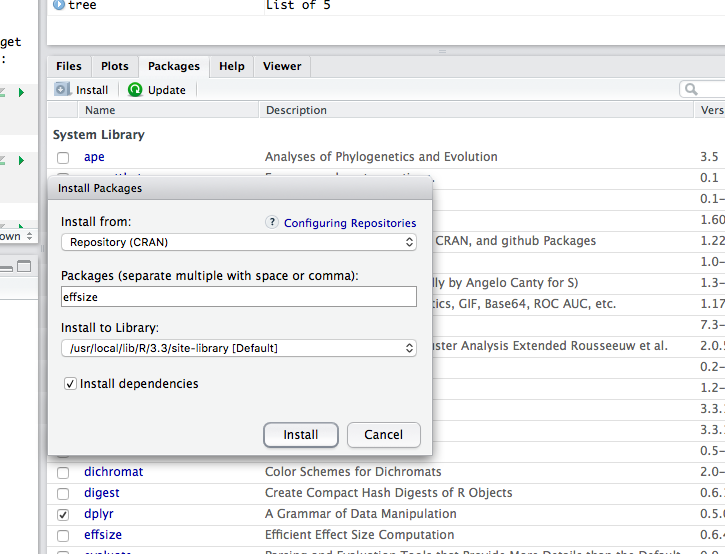
\includegraphics{fig/package_install.png}
\caption{Installing Packages}
\end{figure}

\hypertarget{development-packages---gradethis-and-itssl}{%
\subsection{\texorpdfstring{Development packages - \texttt{gradethis} and \texttt{itssl}}{Development packages - gradethis and itssl}}\label{development-packages---gradethis-and-itssl}}

\texttt{gradethis} is a development package that allows us to use interactive tutorials, but it is somewhat new and still under development so we need to install it manually using \texttt{devtools}.

\begin{enumerate}
\def\labelenumi{\arabic{enumi}.}
\tightlist
\item
  In the \texttt{Console} tab in the lower left panel of RStudio type \texttt{devtools::install\_github("rstudio-education/gradethis")}
\item
  When you are asked
\end{enumerate}

\begin{verbatim}
>These packages have more recent versions available.
  It is recommended to update all of them.
  Which would you like to update?
\end{verbatim}

Select \texttt{1:\ All}

\texttt{itssl} is a new package that contains all the materials including the exercises for this handbook. As it isn't fully certified yet you need to install it using \texttt{devtools}.

\begin{enumerate}
\def\labelenumi{\arabic{enumi}.}
\tightlist
\item
  In the \texttt{Console} tab in the lower left panel of RStudio type \texttt{devtools::install\_github("danmaclean/itssl")}
\end{enumerate}

\hypertarget{using-the-itssl-package}{%
\section{\texorpdfstring{Using the \texttt{itssl} package}{Using the itssl package}}\label{using-the-itssl-package}}

\texttt{itssl} is a package developed solely to accompany this course, the initialism stands for \texttt{intro\ to\ stats\ SL}. Once it is installed you can load it as usual - \texttt{library(itssl)}

All the functions in \texttt{itssl} follow this naming scheme \texttt{its\_\textless{}something-something\textgreater{}\_time()} so you'll be able to spot them as you read along. The main purpose of the functions is to make the course easier to follow and stop us from getting bogged down in a lot of circumstantial code that isn't directly related to our current point, which will usually be statistical rather than related to programming, hence you'll be able to get a lot out of this course even if you haven't used much R before.

If you do have a desire to see the code inside the \texttt{itssl} functions it is available at \url{https://github.com/danmaclean/itssl/tree/master/R}

\hypertarget{acknowledgements}{%
\section{Acknowledgements}\label{acknowledgements}}

This handbook would not have been possible without helpful inspiration from these web pages and leaders in statistical education, please check out their sites.

\begin{itemize}
\tightlist
\item
  \href{https://learningstatisticswithr.com/}{Danielle Navarro - Learning Statistics with R}
\item
  \href{https://statisticsbyjim.com/}{Jim Frost - Statistics By Jim}
\item
  \href{https://lindeloev.github.io/tests-as-linear/}{Jonas Kristoffer Linedlov}
\end{itemize}

\hypertarget{motivation}{%
\chapter{Motivation}\label{motivation}}

Statistics is a word that rhymes with sadistics. Many people have noted this similarity and have felt that sadistics is what was really meant. Admittedly, statistics is hard, even statisticians find it hard. So why on earth would we want to do it? The main reason is because we want to be able to trust in our results as objectively as possible and applying some statistics can help us to do that.

For reasons beyond their control, during their education a lot of biologists with a molecular or biochemistry or genetics or field background develop only a vague conceptual framework about statistics, one that leaves them with the idea that it is all about picking the right test and then they're ok. Often they have gone through a graduate course that introduced them to a lot of tests and a lot of conditions that must be fulfilled and they have gained the impression that there is one `right' test to use in any given situation, which isn't true. Later on this misapprehension is reinforced by the good intentions of colleagues and reviewers with apparently eidetic memories that seem to remember all the conditions and can suggest the `right' test to them in lab meetings or during manuscript revision. Many don't get an experience where there is a sense of working through a statistical problem logically or a discussion of ways of thinking about the problem.

As a result many of us get the sense that everything to do with statistics is arbitrary and dislocated without any logical binding thread. If your prior experience has left you feeling that statistics is a bit of an incomprehensible mess, then this course is for you.

The aim of this course is to introduce a simple new tool and a way of thinking about statistics that can enlighten and simplify all the tests we commonly use as biologists. It may surprise you that this tool will be based on a simple formula for a straight line, something you probably already know. We will look at the bare bones of this and see how it relates to significance tests and see how by thinking of straight lines in your work then you can apply complicated analyses quickly and importantly come to a clearer understanding of the hypotheses you are testing.

Happy \sout{sadisticating} statistics-ing!

\hypertarget{background}{%
\chapter{Background}\label{background}}

\begin{enumerate}
\def\labelenumi{\arabic{enumi}.}
\tightlist
\item
  Questions
\end{enumerate}

\begin{itemize}
\tightlist
\item
  Why do we need statistics?
\item
  What is a null model?
\item
  What is significance?
\end{itemize}

\begin{enumerate}
\def\labelenumi{\arabic{enumi}.}
\setcounter{enumi}{1}
\tightlist
\item
  Objectives
\end{enumerate}

\begin{itemize}
\tightlist
\item
  Understand what the aim of a statistical analysis is
\item
  Understand what a null model is for
\item
  Understand \(p\)-value informally
\end{itemize}

\begin{enumerate}
\def\labelenumi{\arabic{enumi}.}
\setcounter{enumi}{2}
\tightlist
\item
  Keypoints
\end{enumerate}

\begin{itemize}
\tightlist
\item
  We do statistics to be reasonably certain that differences are `real'
\item
  A \(p\)-value describes how often the observed difference occurs according to a default situation we choose
\item
  The slope of a line can help us think about whether two numbers are different.
\end{itemize}

\hypertarget{null-models}{%
\section{Null Models}\label{null-models}}

We all know that doing the same experiment twice will return different results each time. Perhaps not massively different, but definitely not exactly the same. Variation like this can make it hard for us to assert that there are differences between the things we are testing. This is the central issue that statistics seeks to address, in plain English we ask

\begin{myquote}
How can I be reasonably certain that the difference I see is a real one?
\end{myquote}

the answer to this in statistics is usually the same one - compare it to the situation where there isn't any difference, if it is an unlikely result there, then perhaps there is a difference. This `situation where there isn't any difference' is called a Null Model, or perhaps you can think of it as a random model or a default model.

And that's the whole of the logic to a statistical test - we simply make an assumption about what a Null Model of no difference is, then use it to see how likely a given difference would be.

\begin{sidenote}
Just because the overall answer is usually the same one, that doesn't mean that there is only one way of generating a Null Model. Far from it! The selection of the Null Model is one of the thorniest issues in statistics and is one of the reasons most often cited for selecting one type of test over another. Often the Null Model will be the Normal Distribution, which you may have heard of (and yes, it's called the Normal because it's the one we normally use) other common ones are the Binomial or Poisson, the exponential, the Gamma and the \(t\) and \(\chi-squared\). Thankfully, the tool we are going to learn will be able to use all of these appropriately. For most of this book our focus will be on Normal Null Models.
\end{sidenote}

A Null Model will always have some way of incorporating variability, if you ask for a likelihood of a given difference, there will always be an effect of variability on the likelihood, usually the as variability increases the likelihood that there is a difference decreases.

Either way, for our purposes the basic idea is that we look inside the null model and see how likely it would be. Usually we ask a very specific question of a Null Model

\begin{myquote}
What is the likelihood of getting the difference we observed if the true difference were 0, given the observed amount of variablility?
\end{myquote}

The likelihood of the difference under the Null Model is expressed as a very misunderstood and abused quantity - the \(p\)-value.

\hypertarget{p-values}{%
\section{\texorpdfstring{\(p\)-values}{p-values}}\label{p-values}}

A lot of researchers get the impression that \(t\)-tests, ANOVAs and other hypothesis tests tell you whether something is significant with probability \(p\). This is quite a misinterpretation. They do no such thing. More accurately but still rather informally and in general \(p\) can be taken as follows

\begin{myquote}
\(p\) is the likelihood of seeing a difference of the size observed in the Null Model
\end{myquote}

Remembering that the Null Model is the default situation where the difference is 0 then this is resolutely not the same as saying they are definitely different. Just that they're not likely to be the same. The \(p\) in \(p\) value is usually taken to mean `probability', but if it stands for anything it should be `probably not the same'.

Hypothesis testing like this has been criticised for being weak inference, and not without reason. All this means is that we need to be awake to the limitations of our methods.

With this idea of using a Null Model as a reference to see whether our difference is likely or not we can start to think about defining a difference.

\hypertarget{slopes-of-straight-lines-can-help-us-think-about-differences-between-things}{%
\section{Slopes of straight lines can help us think about differences between things}\label{slopes-of-straight-lines-can-help-us-think-about-differences-between-things}}

One way of examining a difference is to think about the slopes of straight lines. It isn't immediately obvious how this works, intuitively we might just want to think about numbers, so let's work through a quick example. Let's consider these data

\begin{Shaded}
\begin{Highlighting}[]
\KeywordTok{library}\NormalTok{(itssl)}
\NormalTok{df <-}\StringTok{ }\KeywordTok{its_bardata_time}\NormalTok{()}
\KeywordTok{its_table_time}\NormalTok{(df)}
\end{Highlighting}
\end{Shaded}

\begin{tabular}{c|c}
\hline
group1 & group2\\
\hline
5.268602 & 7.983835\\
\hline
5.099570 & 7.941177\\
\hline
5.472474 & 6.204316\\
\hline
6.891644 & 7.584074\\
\hline
5.443401 & 7.364379\\
\hline
4.039980 & 6.095724\\
\hline
\end{tabular}

In the beginning of our scientific education we might've plotted them as barcharts, by taking the mean, like this.

\begin{Shaded}
\begin{Highlighting}[]
\KeywordTok{its_barplot_time}\NormalTok{(df)}
\end{Highlighting}
\end{Shaded}

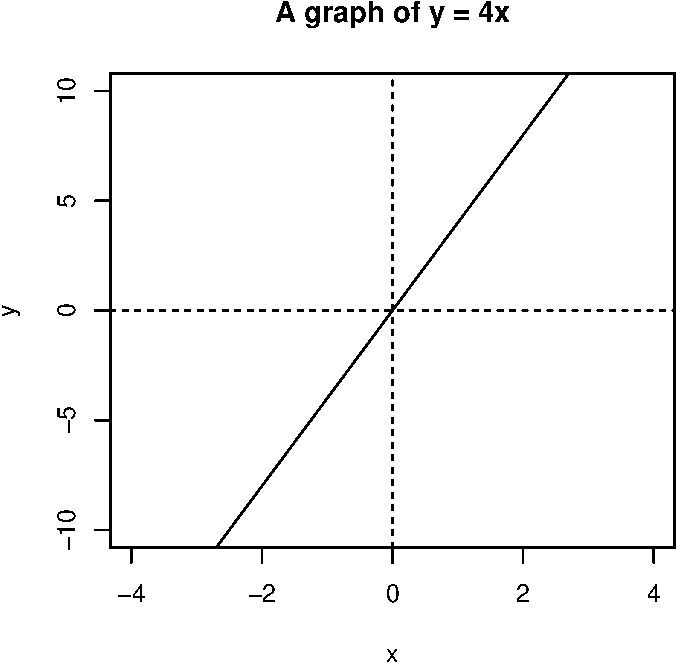
\includegraphics{intro_to_stats_files/figure-latex/unnamed-chunk-7-1.pdf}

Imagine drawing a line between the tops of the bars, like this:

\begin{Shaded}
\begin{Highlighting}[]
\KeywordTok{its_barplot_time}\NormalTok{(df, }\DataTypeTok{join_tops =} \OtherTok{TRUE}\NormalTok{)}
\end{Highlighting}
\end{Shaded}

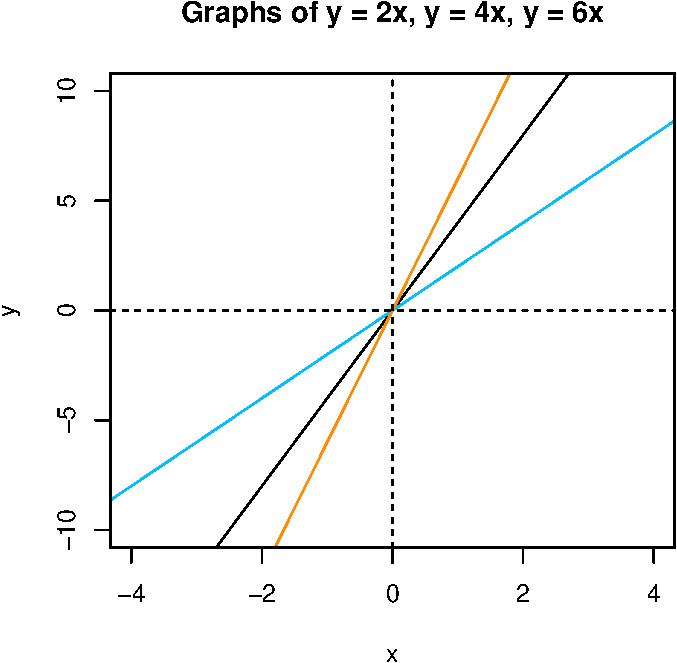
\includegraphics{intro_to_stats_files/figure-latex/unnamed-chunk-8-1.pdf}

The slope of that line tells us about the difference in the means. If it is flat there's no difference, if it isn't flat maybe there is a difference.

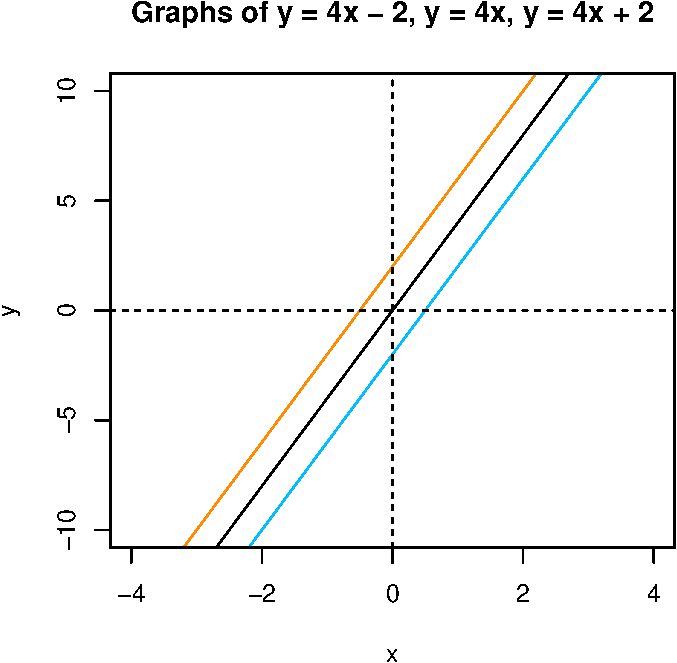
\includegraphics[width=0.5\linewidth]{intro_to_stats_files/figure-latex/unnamed-chunk-9-1} 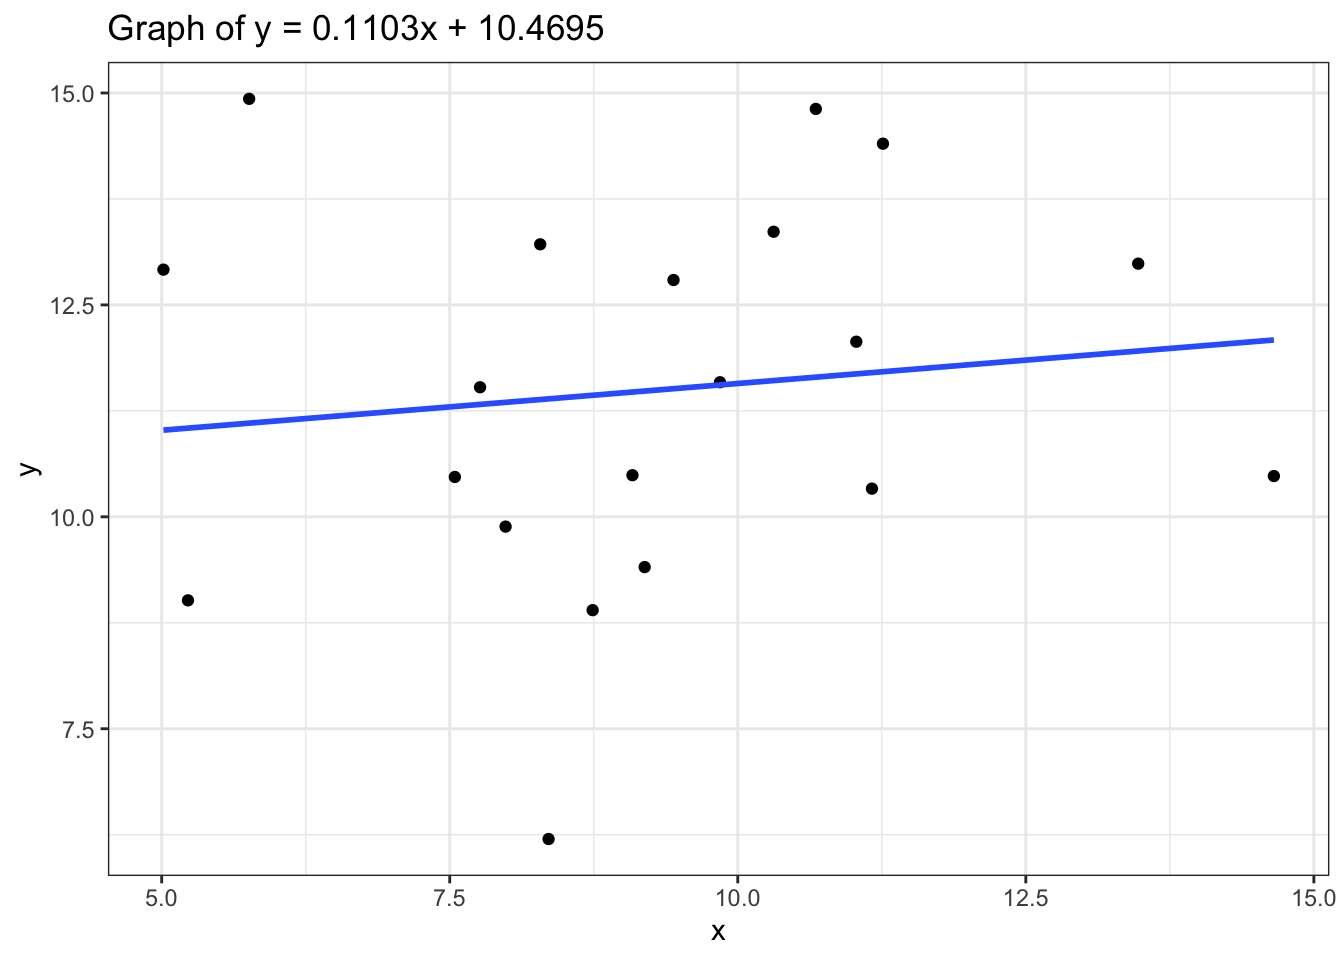
\includegraphics[width=0.5\linewidth]{intro_to_stats_files/figure-latex/unnamed-chunk-9-2}

Now we have a conceptual tool for thinking about differences (like differences in means of samples) as a slope between the means from one group to another. And that is the logic we will be following in this little book. All we will do is learn to look for a slope of a line. We'll look at using a statistical tool called a linear model, which tries to create a straight line that matches the data, so it contains the equation of a straight line but elaborates on the equation alone by providing measures of believability about the slope and other things. The technique we will learn will give us a framework for thinking about performing hypothesis testing in all sorts of comparisons including \(t\)-tests, ANOVA, etc. and with elaborations we'll be able to see how to use the same framework for the other class of tests that we often use, the non-parametric tests.

\begin{roundup}
\begin{itemize}
\tightlist
\item
  We do statistics to be reasonably certain that differences we observe don't occur by chance.

  \begin{itemize}
  \tightlist
  \item
    A \(p\) value doesn't tell us the probability of a result. It tells us how often we would see the observed result in an idealised and simplisitic situation.
  \item
    The slope of a line can help us think about whether two numbers are different.
  \end{itemize}
\end{itemize}
\end{roundup}

\hypertarget{the-linear-model}{%
\chapter{The Linear Model}\label{the-linear-model}}

\begin{enumerate}
\def\labelenumi{\arabic{enumi}.}
\tightlist
\item
  Questions
\end{enumerate}

\begin{itemize}
\tightlist
\item
  How do we describe a straight line?
\item
  What is a Linear Model?
\item
  How \emph{exactly} does a straight line and a linear model help us determine differences?
\end{itemize}

\begin{enumerate}
\def\labelenumi{\arabic{enumi}.}
\setcounter{enumi}{1}
\tightlist
\item
  Objectives
\end{enumerate}

\begin{itemize}
\tightlist
\item
  Understand the parameters of a straight line
\item
  Understand the statistical components of a linear model
\item
  Understand how a sloped line implies a difference in a linear model
\end{itemize}

\begin{enumerate}
\def\labelenumi{\arabic{enumi}.}
\setcounter{enumi}{2}
\tightlist
\item
  Keypoints
\end{enumerate}

\begin{itemize}
\tightlist
\item
  Straight lines have two parameters
\item
  Linear models contain statistics
\item
  Linear models can tell us whether a slope is likely flat or not given the data
\end{itemize}

\hypertarget{from-straight-lines-to-data}{%
\section{From straight lines to data}\label{from-straight-lines-to-data}}

Now that we've decided to use the straight line as our Null Model, with a flat line being the case where there is no difference and a sloped line being otherwise, we need to start to think about lines and a statistical relative called a Linear Models. Linear models are a tool that are similar to a line of best fit, with measures of the variability of the data points that go in to building them. The linear model will be how we bring statistical rigour into our conceptual tool of using straight lines to think about differences. In this section we'll look at them in some detail, but first we'll recap some facts about straight lines.

\hypertarget{straight-line-relationships-are-described-using-two-parameters}{%
\section{Straight line relationships are described using two parameters}\label{straight-line-relationships-are-described-using-two-parameters}}

Its all about \(y = ax + b\) (or \(y = mx + c\), depending on where you went to school). These two equivalent formulae are the standard high-school equations for describing a straight line. They represent how the quantity \(y\) changes as \(x\) does.

As a refresher, \(a\) tells us how much \(y\) increases for every unit increase in \(x\). Here's an example for the equation \(y = 4x\)

\begin{Shaded}
\begin{Highlighting}[]
\KeywordTok{library}\NormalTok{(itssl)}
\KeywordTok{its_axplusb_time}\NormalTok{(}\DataTypeTok{a =} \DecValTok{4}\NormalTok{)}
\end{Highlighting}
\end{Shaded}

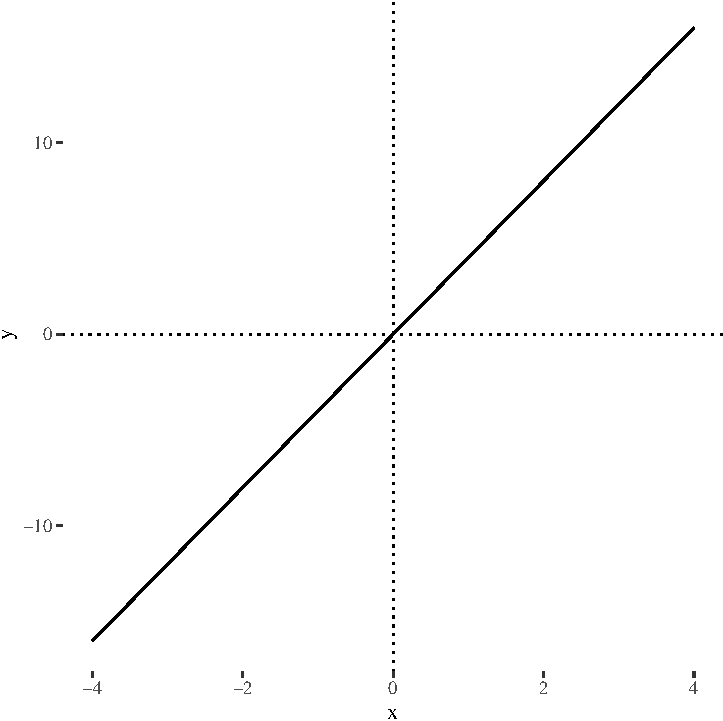
\includegraphics{intro_to_stats_files/figure-latex/unnamed-chunk-11-1.pdf}

If we play about with that value, the slope of the line changes, the \(a\) term is known as the slope, or gradient, or more often because it is just a multiplier of \(x\) its called the coefficient. Here's some different coefficients just to prove that point

\begin{Shaded}
\begin{Highlighting}[]
\KeywordTok{its_axplusb_time}\NormalTok{(}\DataTypeTok{a =} \DecValTok{4}\NormalTok{) }\OperatorTok{+}
\StringTok{  }\KeywordTok{its_add_line_time}\NormalTok{(}\DataTypeTok{a =} \DecValTok{2}\NormalTok{, }\DataTypeTok{colour =} \StringTok{"deepskyblue"}\NormalTok{) }\OperatorTok{+}
\StringTok{  }\KeywordTok{its_add_line_time}\NormalTok{(}\DataTypeTok{a =} \DecValTok{6}\NormalTok{, }\DataTypeTok{colour =} \StringTok{"darkorange"}\NormalTok{)}
\end{Highlighting}
\end{Shaded}

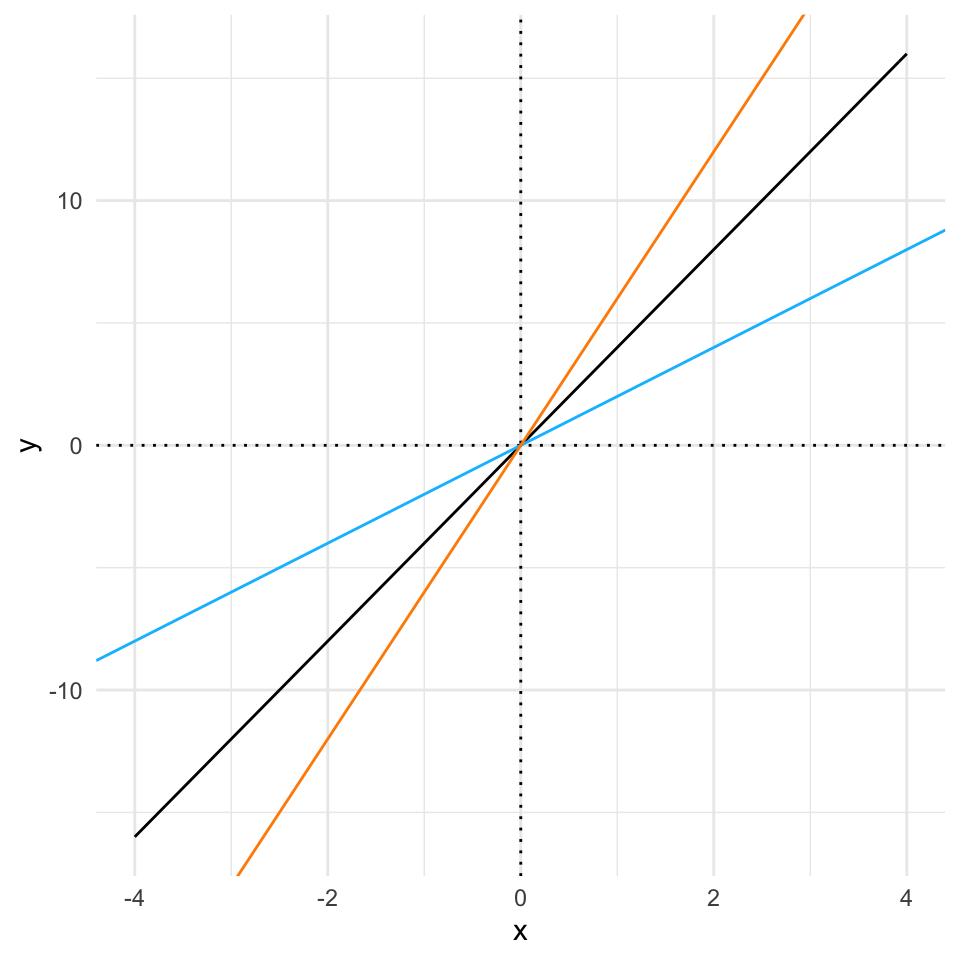
\includegraphics{intro_to_stats_files/figure-latex/unnamed-chunk-12-1.pdf}

The \(b\) part of the formula just tells us how much we add on to \(y\) after we've calculated the coefficient effect. It has the effect of pushing the line up and down the y-axis. When we look at the value of \(y\) for \(x = 0\) we get the position that the graph hits the y-axis so this number is often called the intercept. Here's a set of lines to show that.

\begin{Shaded}
\begin{Highlighting}[]
\KeywordTok{its_axplusb_time}\NormalTok{(}\DataTypeTok{a =} \DecValTok{4}\NormalTok{, }\DataTypeTok{b =} \DecValTok{0}\NormalTok{) }\OperatorTok{+}\StringTok{ }
\StringTok{  }\KeywordTok{its_add_line_time}\NormalTok{(}\DataTypeTok{a =} \DecValTok{4}\NormalTok{, }\DataTypeTok{b =} \DecValTok{-2}\NormalTok{, }\DataTypeTok{colour =} \StringTok{"deepskyblue"}\NormalTok{) }\OperatorTok{+}
\StringTok{  }\KeywordTok{its_add_line_time}\NormalTok{(}\DataTypeTok{a =} \DecValTok{4}\NormalTok{, }\DataTypeTok{b =} \DecValTok{2}\NormalTok{, }\DataTypeTok{colour =} \StringTok{"darkorange"}\NormalTok{)}
\end{Highlighting}
\end{Shaded}

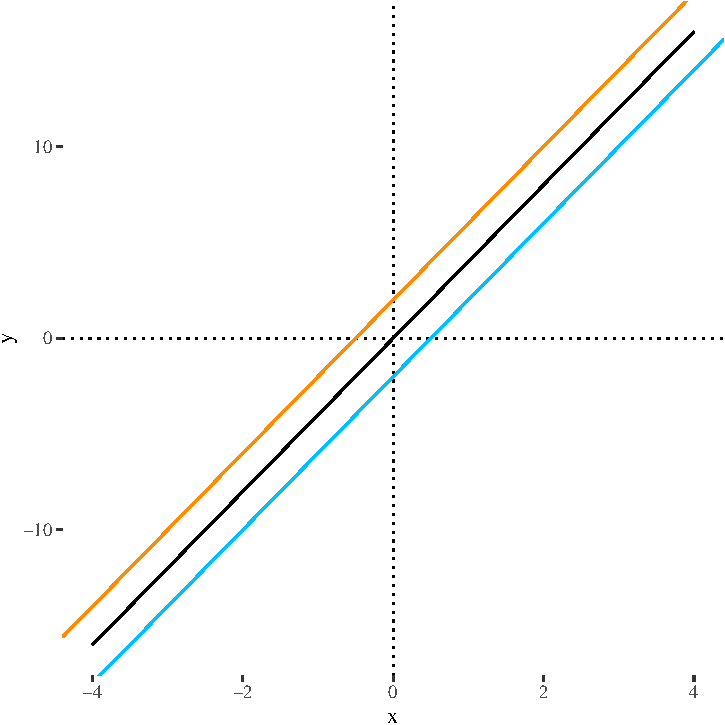
\includegraphics{intro_to_stats_files/figure-latex/unnamed-chunk-13-1.pdf}

That's all we need to know about the equation of the straight line. Now we need to look at how they're a useful tool when analysing experimental data.

\hypertarget{linear-models-try-to-create-a-linear-equation-from-data}{%
\section{Linear models try to create a linear equation from data}\label{linear-models-try-to-create-a-linear-equation-from-data}}

A linear model is a simplification of the relationship between some sets of numbers (in the simple case we will introduce here, it is two sets, but it can be more). At its heart is a straight line, with the equation we discussed above and a certain set of values for \(a\) (the coefficient) and \(b\) the intercept, along with some statistics that describe the strength of the relationship.

Let's walk through building one, graphically and in R.

First we need some sets of values, \(x\) and \(y\). Usually, these would be from an experiment, but here I'll make some toy ones.

\begin{Shaded}
\begin{Highlighting}[]
\NormalTok{df <-}\StringTok{ }\KeywordTok{its_random_xy_time}\NormalTok{(}\DecValTok{20}\NormalTok{)}
\KeywordTok{its_plot_xy_time}\NormalTok{(df)}
\end{Highlighting}
\end{Shaded}

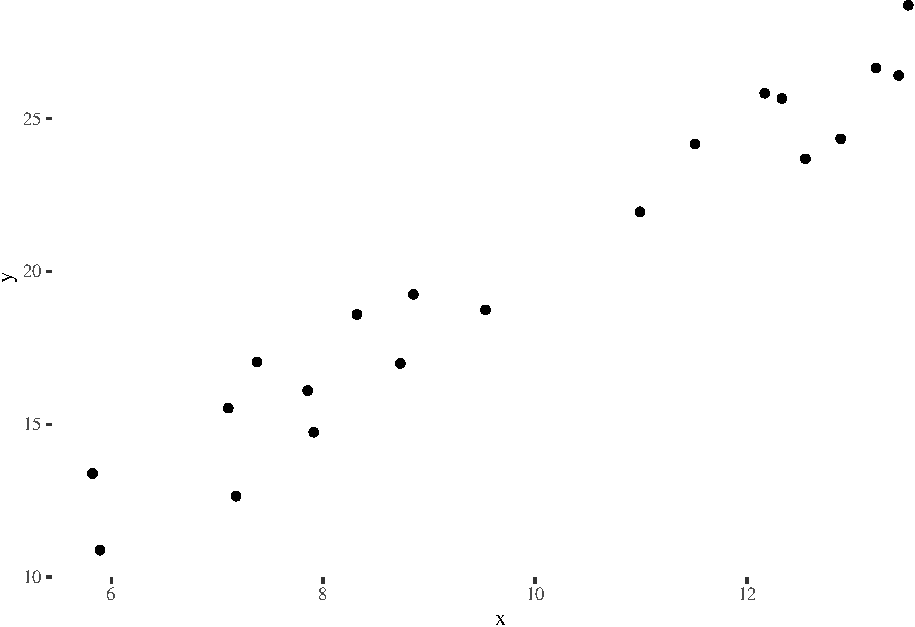
\includegraphics{intro_to_stats_files/figure-latex/unnamed-chunk-14-1.pdf}

The graph shows 20 random \(x\) values between 5 and 15 plotted against 20 \(y\) values which are calculated as \(2x\) with a little random noise added. We can see that there is definitely a relationship (not least because we engineered it that way). The objective of the linear model is to quantify and describe the relationship in some way. Here's where the linear equation comes in, if we could come up with a line that fitted through the data we could use the linear equation of that line to roughly describe - or model - our data. Skipping to the end a bit, then there is absolutely a way to get the line from the data. The methods are described in lots of statistics books so I won't repeat them, but you may be familiar with the general methods, it's the `line of best fit' according to the ordinary least squares method. Details aside, the actual linear model function we need in R is \texttt{lm()} and it works like this

\begin{Shaded}
\begin{Highlighting}[]
\KeywordTok{lm}\NormalTok{(y }\OperatorTok{~}\StringTok{ }\NormalTok{x, }\DataTypeTok{data =}\NormalTok{ df)}
\end{Highlighting}
\end{Shaded}

That's it! The function \texttt{lm()} does the work, it takes a fairly odd syntax, though. The \texttt{y\ \textasciitilde{}\ x} bit is an R formula and describes the relationship you want to examine, you can read it as \texttt{y\ depends\ on\ x}. The \texttt{y} and \texttt{x} we're referring to here are the two columns of numbers we created and plotted above, the \texttt{data} argument just says in which object to look for the data.

Looking at the function output we get this

\begin{verbatim}
## 
## Call:
## lm(formula = y ~ x, data = df)
## 
## Coefficients:
## (Intercept)            x  
##       0.778        1.955
\end{verbatim}

These are the intercept (\(b\)) and the coefficient of \(x\) (\(a\)) that we need to describe the line. So our data are described by the line \(y = 1.955x + 0.778\).

So this line is a model of the data, it's a model in the sense that it is something that represents our data, but isn't it. Looking at them together we can see the model and the data it stands for.

\begin{Shaded}
\begin{Highlighting}[]
\KeywordTok{its_plot_xy_time}\NormalTok{(df, }\DataTypeTok{line =} \OtherTok{TRUE}\NormalTok{)}
\end{Highlighting}
\end{Shaded}

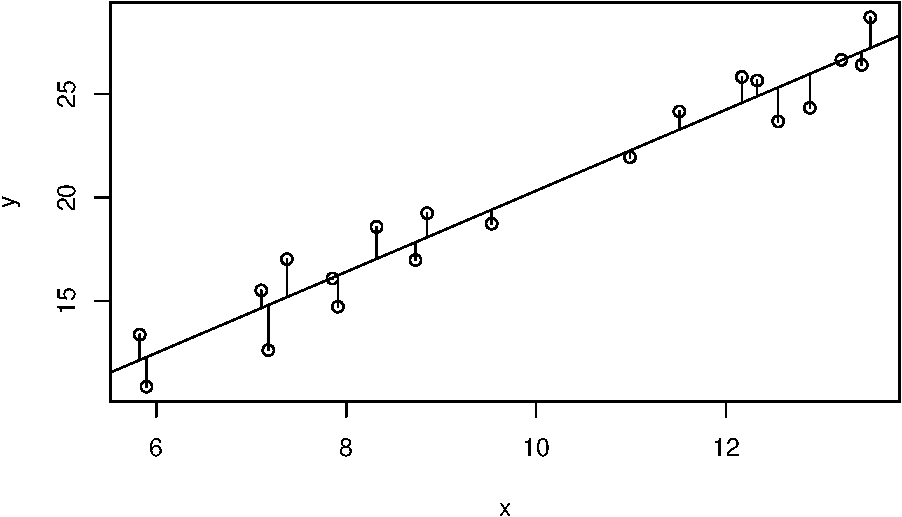
\includegraphics{intro_to_stats_files/figure-latex/unnamed-chunk-17-1.pdf}

The line alone can be useful to teach us about our data, but there's more to the linear model than just the line.

\hypertarget{linear-models-describe-relationships-between-variables}{%
\section{Linear models describe relationships between variables}\label{linear-models-describe-relationships-between-variables}}

Beyond working out the equation of the line, the linear model process aims to quantify and describe relationships between the variables in the data, in our toy example the variables are \(x\) and \(y\). Specifically when we say `relationship', we mean whether a change in the value of \(x\) appears to go along with some change in the value of \(y\).

In other words, we can think of relationship as being the slope. If \(x\) causes some change in \(y\) when we plot it then there must be a slope. We call the slope \(a\) in our equation of a line and we call it the coefficient of the \(x\) term in our linear model. These are all equivalent interpretations for our purposes, slope, relationship, coefficient.

Linear models calculate statistics to help us decide whether the coefficient/slope/\(a\) of the relationship we observe is important or not.

\hypertarget{not-all-lines-of-best-fit-are-equally-good}{%
\section{Not all lines of best fit are equally good}\label{not-all-lines-of-best-fit-are-equally-good}}

Although a line of best fit can always be calculated, the line might not be worth much. Consider two sets of very similar numbers. Here's two vectors of random numbers with the same mean and their plot.

\begin{Shaded}
\begin{Highlighting}[]
\NormalTok{more_df <-}\StringTok{ }\KeywordTok{data.frame}\NormalTok{(}
\NormalTok{  x <-}\StringTok{ }\KeywordTok{runif}\NormalTok{(}\DecValTok{20}\NormalTok{, }\DecValTok{5}\NormalTok{, }\DecValTok{15}\NormalTok{),}
\NormalTok{  y <-}\StringTok{ }\KeywordTok{runif}\NormalTok{(}\DecValTok{20}\NormalTok{, }\DecValTok{5}\NormalTok{, }\DecValTok{15}\NormalTok{)}
\NormalTok{)}

\KeywordTok{its_plot_xy_time}\NormalTok{(more_df)}
\end{Highlighting}
\end{Shaded}

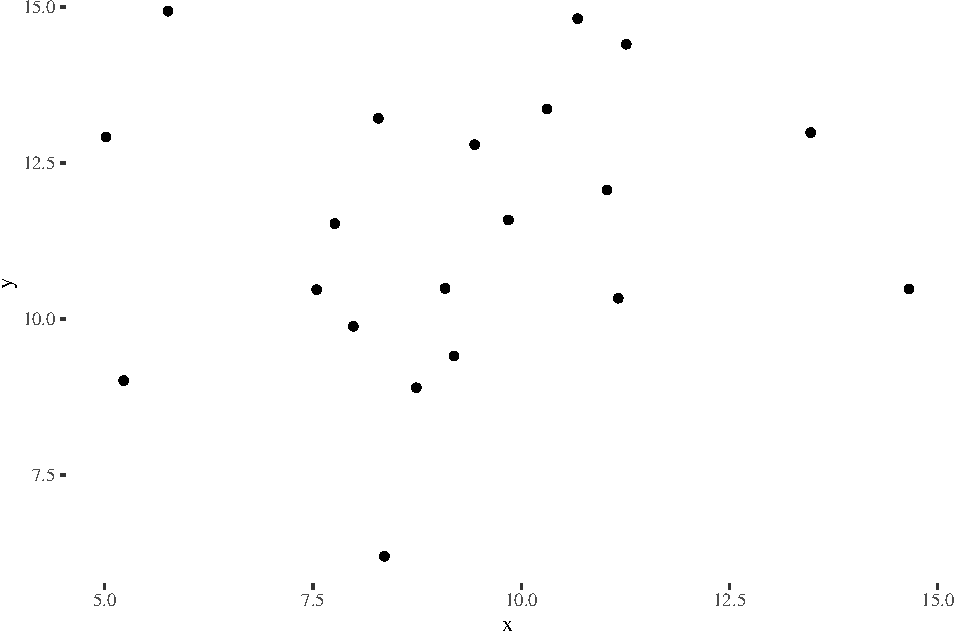
\includegraphics{intro_to_stats_files/figure-latex/unnamed-chunk-18-1.pdf}

We can definitely calculate a line that fits these,

\begin{Shaded}
\begin{Highlighting}[]
\KeywordTok{lm}\NormalTok{(y }\OperatorTok{~}\StringTok{ }\NormalTok{x, }\DataTypeTok{data =}\NormalTok{ more_df)}
\end{Highlighting}
\end{Shaded}

\begin{verbatim}
## 
## Call:
## lm(formula = y ~ x, data = more_df)
## 
## Coefficients:
## (Intercept)            x  
##     10.4695       0.1103
\end{verbatim}

and it would be \(y = 0.1103x + 10.6495\). But if we compare the fit of those lines, like in these plots

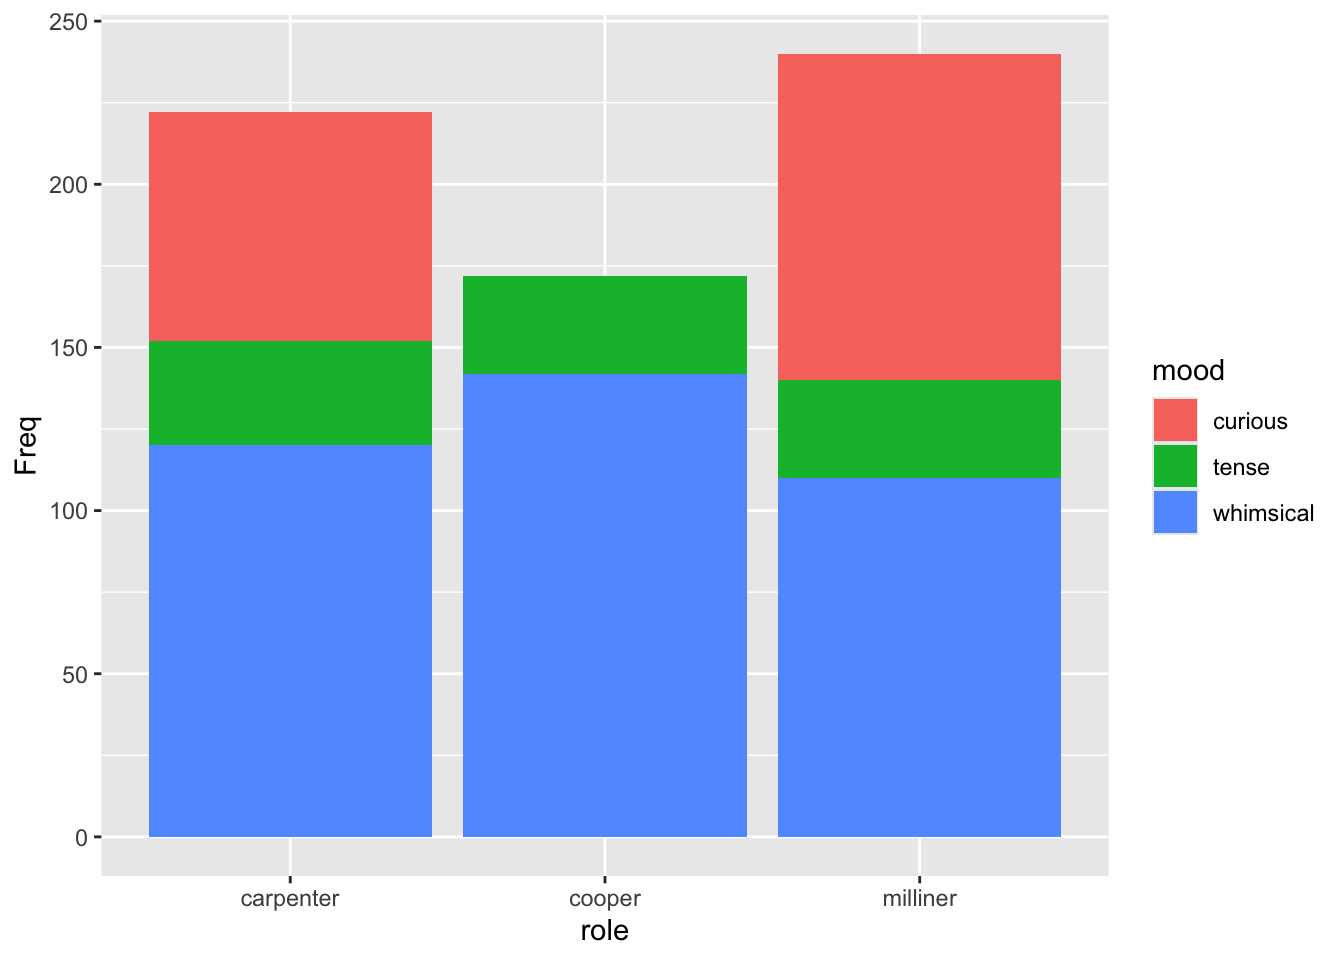
\includegraphics[width=0.5\linewidth]{intro_to_stats_files/figure-latex/unnamed-chunk-20-1} 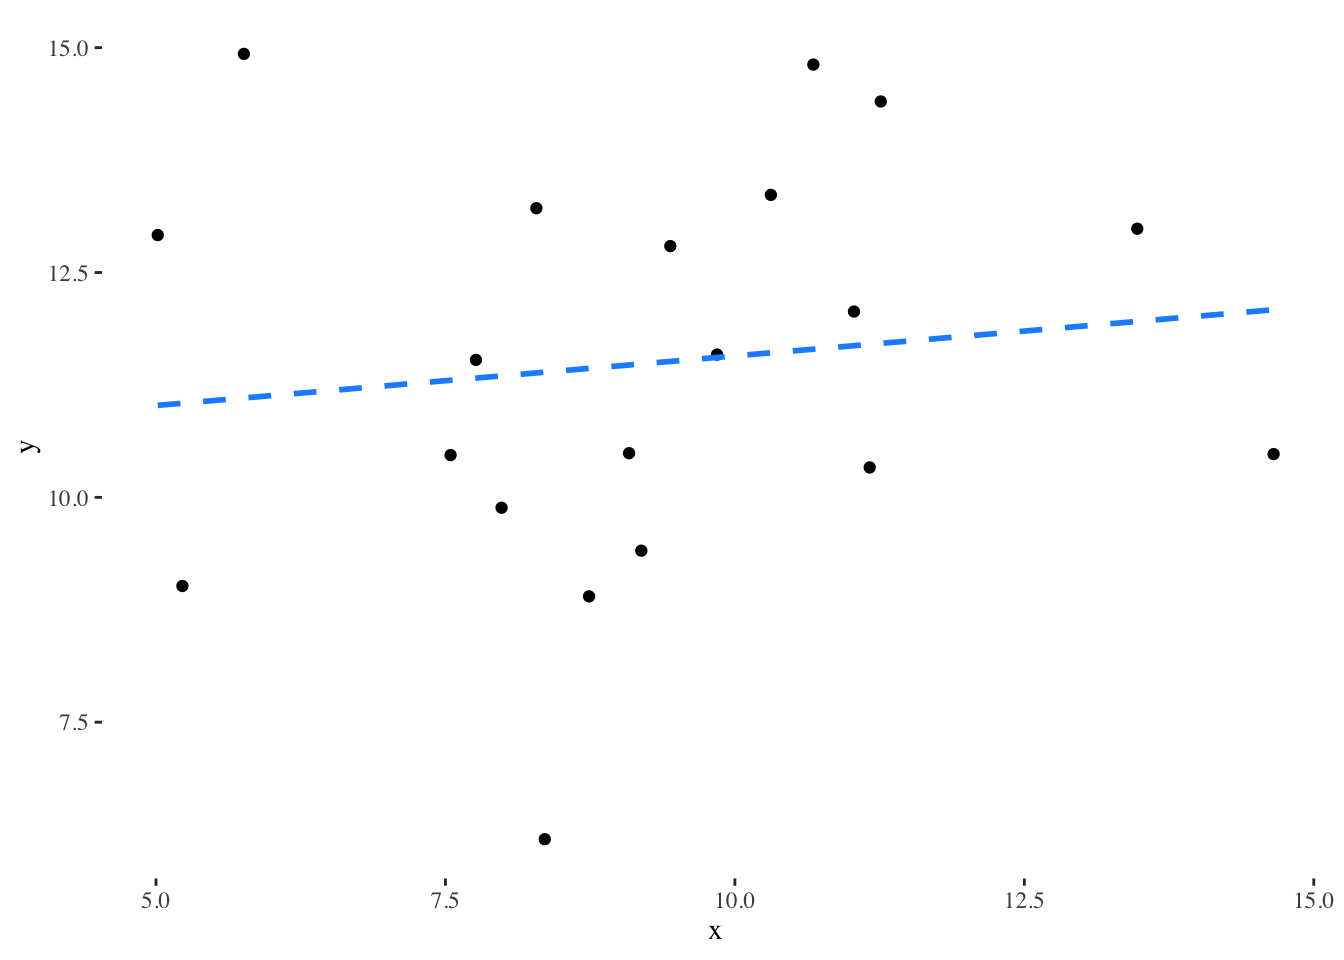
\includegraphics[width=0.5\linewidth]{intro_to_stats_files/figure-latex/unnamed-chunk-20-2}

we can clearly see that not all lines are created equal. The first line fits the data much more closely than the second one. We can also see that the relationship between \(x\) and \(y\) is much weaker in the second set than in the first (the coefficient/slope/\(a\) is weaker. So a sensible linear model of our data would give us not just the equation but also measures of the closeness of fit and therefore believability of the value of slope of the line. In terms of our Null Model flat line/sloped line model this means that when we have a significant coefficient, we are not likely to have a flat line. Let's look at the statistics in the linear model that show us what a significant coefficient is.

\hypertarget{linear-models-contain-statistics-describing-the-goodness-of-the-model}{%
\section{Linear models contain statistics describing the goodness of the model}\label{linear-models-contain-statistics-describing-the-goodness-of-the-model}}

The same function we've already used - \texttt{lm()} - calculates certain statistics. We can print them using the \texttt{summary()} function.

\begin{Shaded}
\begin{Highlighting}[]
\NormalTok{model <-}\StringTok{ }\KeywordTok{lm}\NormalTok{(y }\OperatorTok{~}\StringTok{ }\NormalTok{x, }\DataTypeTok{data =}\NormalTok{ df)}
\KeywordTok{summary}\NormalTok{(model)}
\end{Highlighting}
\end{Shaded}

\begin{verbatim}
## 
## Call:
## lm(formula = y ~ x, data = df)
## 
## Residuals:
##      Min       1Q   Median       3Q      Max 
## -2.17560 -1.00570 -0.01092  1.17016  1.83047 
## 
## Coefficients:
##             Estimate Std. Error t value Pr(>|t|)    
## (Intercept)   0.7780     1.1442    0.68    0.505    
## x             1.9555     0.1122   17.42 1.03e-12 ***
## ---
## Signif. codes:  0 '***' 0.001 '**' 0.01 '*' 0.05 '.' 0.1 ' ' 1
## 
## Residual standard error: 1.303 on 18 degrees of freedom
## Multiple R-squared:  0.944,	Adjusted R-squared:  0.9409 
## F-statistic: 303.6 on 1 and 18 DF,  p-value: 1.027e-12
\end{verbatim}

This output is verbose, there are four blocks.

\begin{enumerate}
\def\labelenumi{\arabic{enumi}.}
\tightlist
\item
  \texttt{Model\ Call} - just a restatement of the function we called
\item
  \texttt{Residuals} - a set of measures of the distribution of the residuals, we'll look at this later.
\item
  \texttt{Coefficients} - the terms of the equation and their statistics; so the intercept (\(b\)) and the coefficient of \texttt{x} (\(a\)) that we've already seen and the \texttt{Estimate} (computed values of those). We see also columns of statistics for each.
\item
  The model level statistics summary - some statistics that apply to the whole model.
\end{enumerate}

Let's start at the bottom and look at model level summary.

\hypertarget{residual-standard-error}{%
\subsection{Residual Standard Error}\label{residual-standard-error}}

This is a measure of how well the line fits the data. In essence Residual Standard Error is the average distance from each real data point to the line, the further the points are from the line (the worse the fit) the bigger the Residual Standard Error. If you look at the plots again with those distances drawn in you can see quite clearly the residual error for the second model is much bigger than for the first.

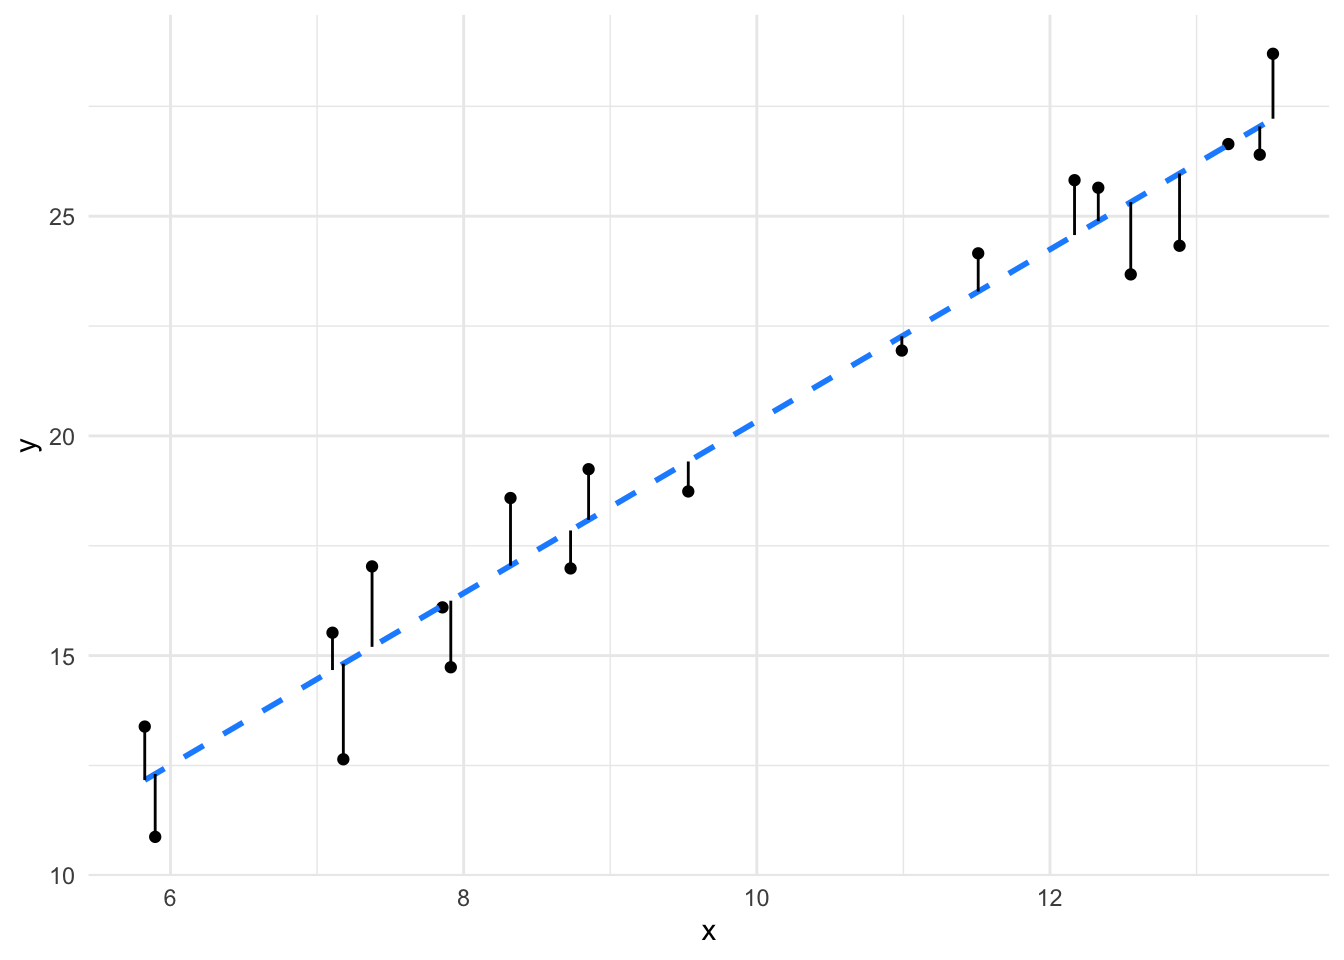
\includegraphics[width=0.5\linewidth]{intro_to_stats_files/figure-latex/unnamed-chunk-22-1} 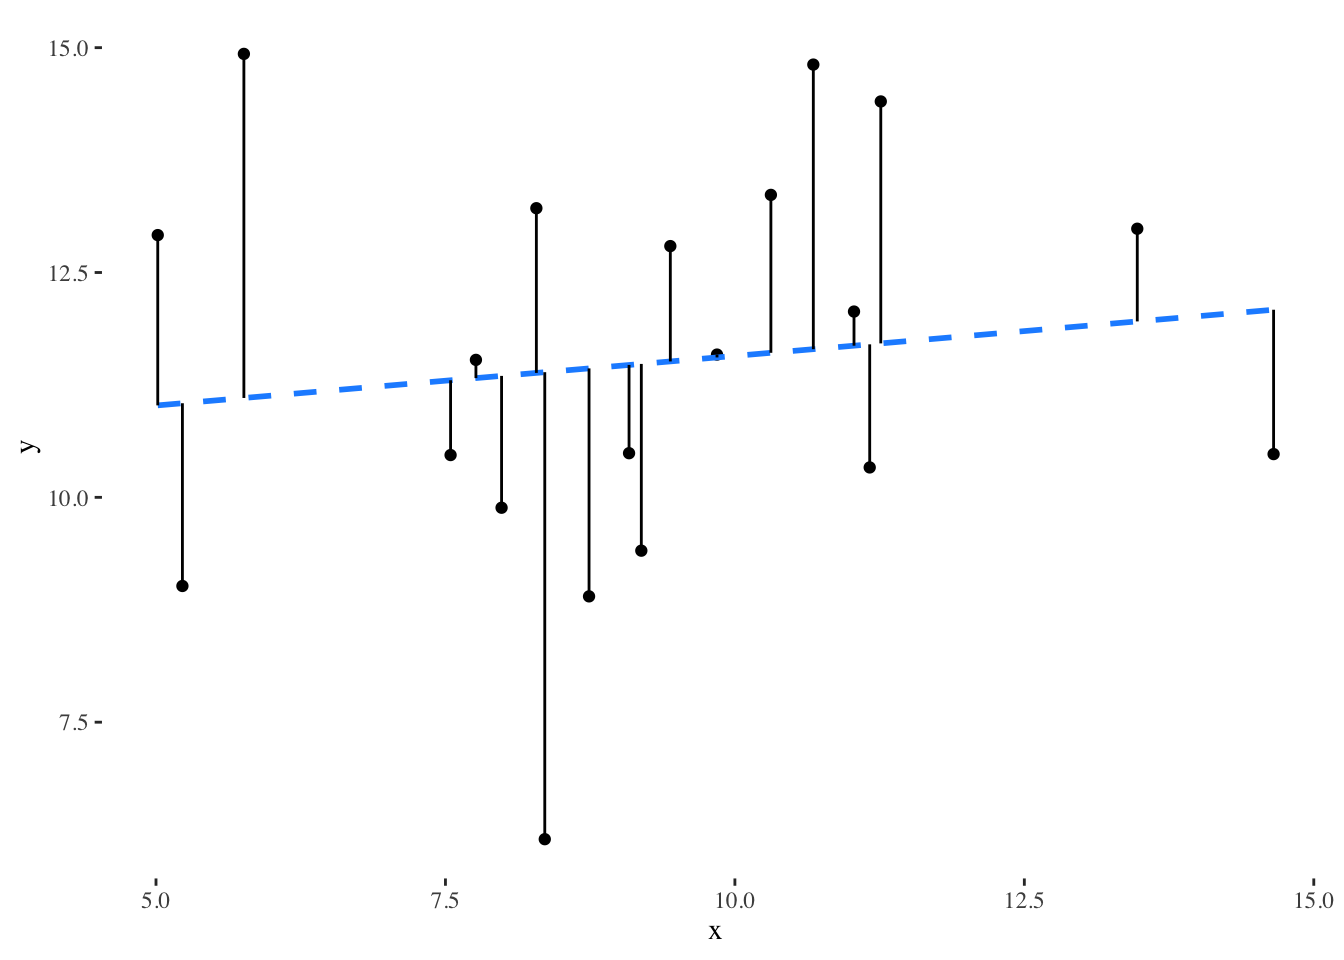
\includegraphics[width=0.5\linewidth]{intro_to_stats_files/figure-latex/unnamed-chunk-22-2}

\begin{sidenote}
We're working hard here to avoid using too much mathematical notation and examination of the mechanics of the linear model, but the residuals are quite an important aspect, so Im going to use this aside to delve just a little deeper. Unlike the linear equation, the linear model has an extra error term, \(e\) which represents the residuals by quantifying the average distance from the actual measurments to the line in the y-axis.

The \(e\) term adds something onto the y value of the whole equation; the bigger \(e\) is the more we need to add on to the value of the \(x\) from the line to get the real \(y\). Logically, the bigger \(e\) is the more the line misses the points in the model overall. The error is a major determinent of whether a model is any good or whether things are significant so it's worth knowing how it relates to the model.
\end{sidenote}

\hypertarget{r2}{%
\subsection{\texorpdfstring{\(R^2\)}{R\^{}2}}\label{r2}}

\(R^2\) is another measure of how well the model fits the data. If you're thinking correlation coefficient here, then you're in the right area. \(R^2\) describes the proportion of variance in the \(y\) values that can be explained by the \(x\) values. The \(R^2\) always falls between 0 and 1. Closer to 1 is usually better, but it is very domain and dataset dependent. With small and biological data sets, we don't always see values close to 1 because of the noise of the system.

The proper one to use in \sout{most} all cases is the \texttt{Adjusted\ R-squared}.

\hypertarget{r2-versus-residual-standard-error}{%
\subsubsection{\texorpdfstring{\(R^2\) versus Residual Standard Error}{R\^{}2 versus Residual Standard Error}}\label{r2-versus-residual-standard-error}}

So what's the difference between these two - at first glance they do the same thing. The major difference is that RSE is in the units of the data and \(R^2\) is in relative units, so you can use them in different situations e.g if you want to make your model work within particular tolerances or you want to compare models in different units.

\hypertarget{f-statistic}{%
\subsection{\texorpdfstring{\(F\)-Statistic}{F-Statistic}}\label{f-statistic}}

The \(F\)-Statistic is an indicator of a relationship between the \(x\) and \(y\) values of the model. In effect \(F\) tests how much better the relationship is in your model than a model in which the relationship is completely random. It's actually a ratio such that when the \(F\)-statistic is at 1, the relationship is no stronger than a random relationship. The further above 1 \(F\) is, the more it is likely there is a real relationship in the model. The \(p\) value here is the \(p\) that this size of \(F\) would occur in a random relationship with a similar dataset size. As with the other statistics, the significance of the actual size of \(F\) is dependent on the domain and data being analysed.

\hypertarget{coefficients-have-statistics}{%
\section{Coefficients have statistics}\label{coefficients-have-statistics}}

Along with these model level statistics, linear modelling with \texttt{lm()} gives us a set of statistics \emph{per coefficient}. These measure the effect that each coefficient has on the output variable \(y\). Basically a significant coefficient, is one that has a non-zero slope and is an important determinant of the value of \(y\).

\hypertarget{estimate}{%
\subsection{Estimate}\label{estimate}}

These are the \texttt{Estimate}, which is the actual value of the coefficient from the model. We will see that along with Intercept we can have models with more than one other coefficient. These are given in the units of the data.

\hypertarget{std.-error}{%
\subsection{Std. Error}\label{std.-error}}

A measure of the variability of the strength of the effect, so if some \(x\) points give more pronounced \(y\) values at similar coefficient values, you get a higher variability of the strength. Generally lower standard error of the coefficient is good.

\hypertarget{t-value}{%
\subsection{\texorpdfstring{\(t\)-value}{t-value}}\label{t-value}}

An estimate of how extreme the coefficient value is, basically how many Standard Deviations away the estimated coefficient is from the centre of a presumed Normal distribution with mean 0. It is absolutely a \(t\)-test \(t\)-value, and like in a \(t\)-test we want it to be high. The higher \(t\) is, then the more likely that the coefficient is not 0.

\hypertarget{wait-what}{%
\subsubsection{Wait, what?}\label{wait-what}}

Why would we care whether the coefficient is 0 or not? Well, because if it is 0, then it's having no effect on the model. Consider again the equation of a line

\begin{equation}
y = ax + b
\end{equation}

If we let the coefficient \(a = 0\), this happens

\begin{equation}
y = 0 x + b\\
y = b
\end{equation}

The coefficient disappears, it's having no effect!

If the coefficient is not many standard deviations away from 0, it's probably not having much effect on the relationship. The \(t\) value tries to work out whether, given the data, the coefficient is in anyway different to 0.

In plainer English, we are really saying that the size if the slope is not likely to be 0. That it is not likely that there is no relationship. Which is weak inference, but is \emph{exactly} the same sort of inference that all the other hypothesis tests make and is exactly the same interpretation.

Of course, this will depend on the size of the standard deviation. The noisier the data or the smaller the sample size then the larger this value will need to be to be important.

\hypertarget{prt}{%
\subsection{\texorpdfstring{\(Pr(>|t|)\)}{Pr(\textgreater\textbar t\textbar)}}\label{prt}}

This weird shorthand expression is just giving the probability of getting a value larger than the \(t\)-value. This comes from a \(t\)-test within the model and takes into account the dataset size and variability, you can think of it as the \(p\)-value of a test asking whether the coefficient is equal to 0. So if \(p\) is less than 0.05 you can say that the value of the coefficient is not likely to be 0 and therefore is having an effect on the model.

\hypertarget{a-non-zero-slope-is-what-matters}{%
\section{A non-zero slope is what matters}\label{a-non-zero-slope-is-what-matters}}

By looking at the \(p\)-value of the coefficient then, we can see whether there is a significant relationship or, more accurately a non-zero slope

We can really emphasise by looking at the plots of lines we looked at earlier.

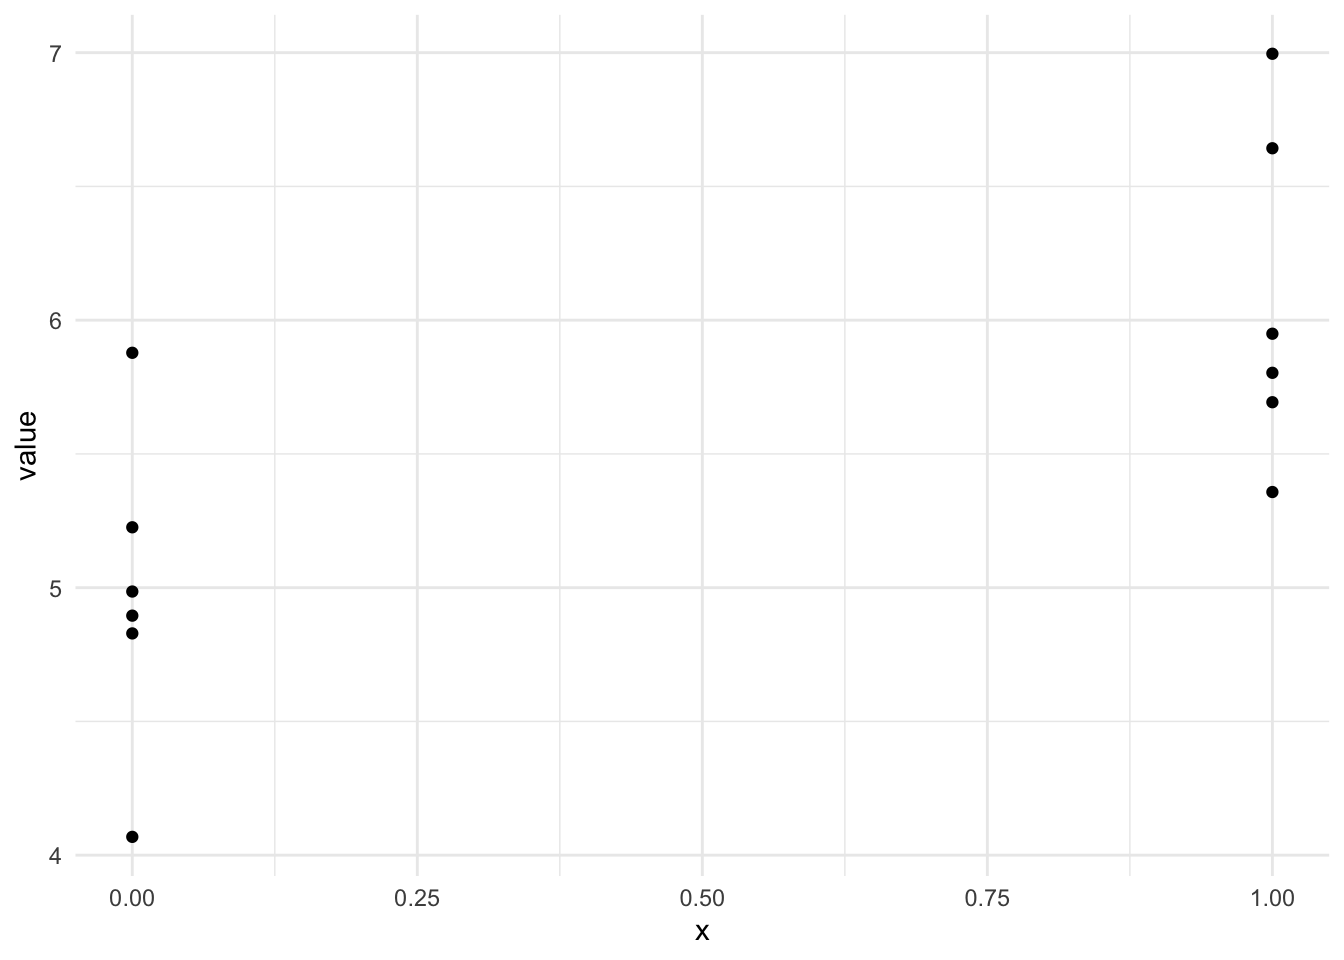
\includegraphics[width=0.5\linewidth]{intro_to_stats_files/figure-latex/unnamed-chunk-24-1} 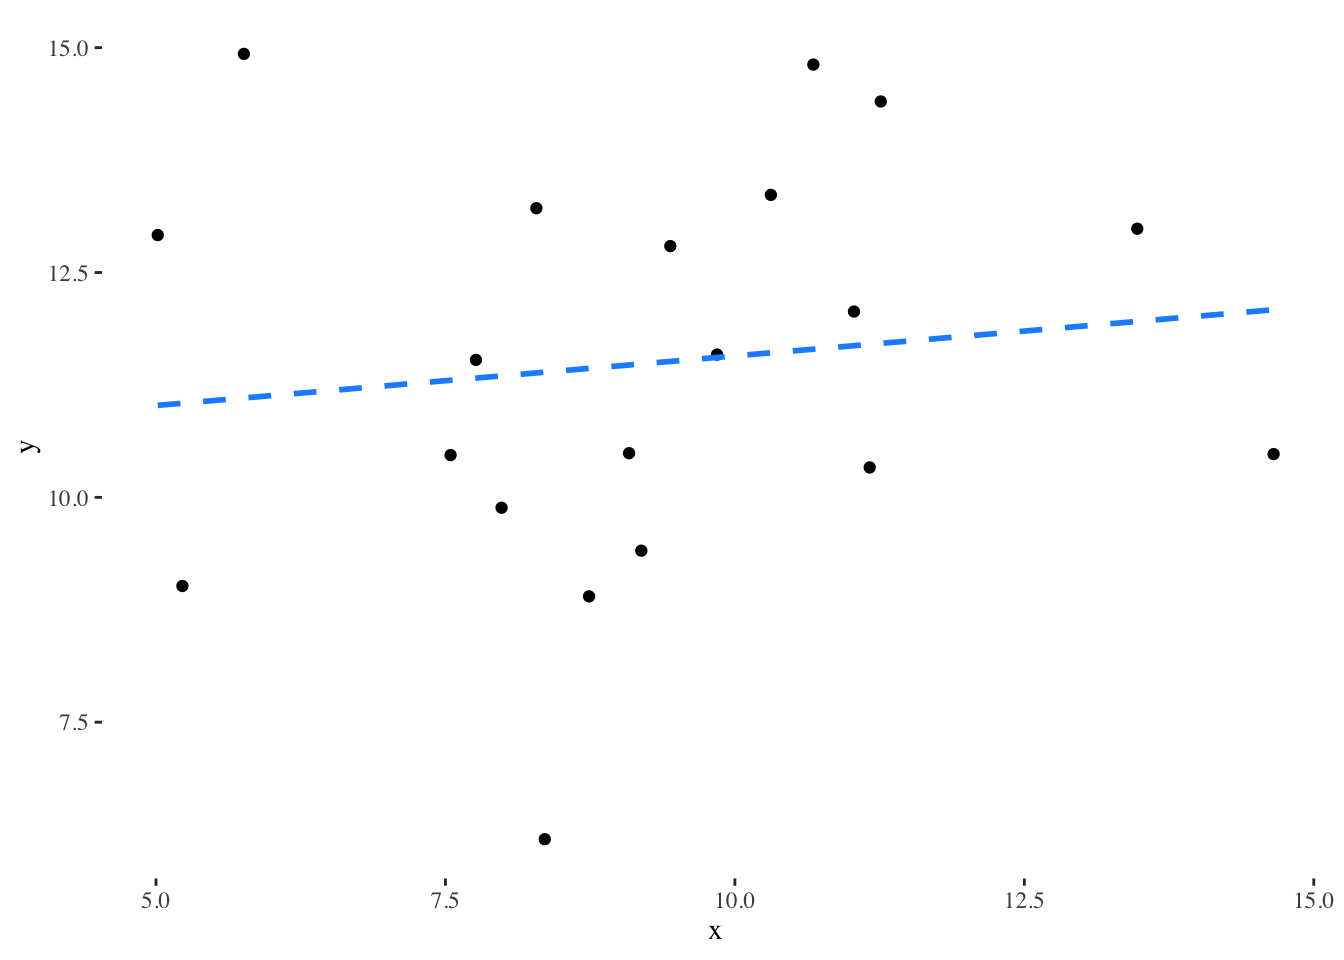
\includegraphics[width=0.5\linewidth]{intro_to_stats_files/figure-latex/unnamed-chunk-24-2}

The slope of the second plot is weaker, it's much flatter - much closer to zero, in fact given the spread of the data we aren't that confident that it isn't a flat (zero) slope, so we aren't that confident that there is a significant relationship.

We can quickly see that definitively using \texttt{lm()} if we compare two models based on those two datasets.

We already built the model for the first slope.

\begin{Shaded}
\begin{Highlighting}[]
\KeywordTok{summary}\NormalTok{(model)}
\end{Highlighting}
\end{Shaded}

\begin{verbatim}
## 
## Call:
## lm(formula = y ~ x, data = df)
## 
## Residuals:
##      Min       1Q   Median       3Q      Max 
## -2.17560 -1.00570 -0.01092  1.17016  1.83047 
## 
## Coefficients:
##             Estimate Std. Error t value Pr(>|t|)    
## (Intercept)   0.7780     1.1442    0.68    0.505    
## x             1.9555     0.1122   17.42 1.03e-12 ***
## ---
## Signif. codes:  0 '***' 0.001 '**' 0.01 '*' 0.05 '.' 0.1 ' ' 1
## 
## Residual standard error: 1.303 on 18 degrees of freedom
## Multiple R-squared:  0.944,	Adjusted R-squared:  0.9409 
## F-statistic: 303.6 on 1 and 18 DF,  p-value: 1.027e-12
\end{verbatim}

Let's also build the model for the second slope, it is in a dataframe called \texttt{more\_df}

\begin{Shaded}
\begin{Highlighting}[]
\NormalTok{model_}\DecValTok{2}\NormalTok{ <-}\StringTok{ }\KeywordTok{lm}\NormalTok{(y }\OperatorTok{~}\StringTok{ }\NormalTok{x, }\DataTypeTok{data =}\NormalTok{ more_df)}
\KeywordTok{summary}\NormalTok{(model_}\DecValTok{2}\NormalTok{)}
\end{Highlighting}
\end{Shaded}

\begin{verbatim}
## 
## Call:
## lm(formula = y ~ x, data = more_df)
## 
## Residuals:
##     Min      1Q  Median      3Q     Max 
## -5.1924 -1.5007  0.1171  1.7748  3.8260 
## 
## Coefficients:
##             Estimate Std. Error t value Pr(>|t|)    
## (Intercept)  10.4695     2.0315   5.154 6.67e-05 ***
## x             0.1103     0.2127   0.519     0.61    
## ---
## Signif. codes:  0 '***' 0.001 '**' 0.01 '*' 0.05 '.' 0.1 ' ' 1
## 
## Residual standard error: 2.296 on 18 degrees of freedom
## Multiple R-squared:  0.01472,	Adjusted R-squared:  -0.04001 
## F-statistic: 0.269 on 1 and 18 DF,  p-value: 0.6103
\end{verbatim}

We can clearly see that the second model is a poorer fit to the data. The model level statistics are less convincing: \(F\) is reduced to 0.269 (from 303.6), the \(p-value\) shows the difference occurs by chance 61 \% of the time and the \texttt{Adjusted\ R-squared} is close to 0, indicating a poor relationship. The coefficient was measurable, but it is not significant (and not coincidentally) occurring by chance 61 \% of the time. The slope therefore is not significantly different from 0 and \(x\) in \texttt{model\_2} appears to have no effect on \(y\).

It is this slope assessing feature of the linear models that will help us in our overall goal of using the linear model to do the work of all the other statistical tests we commonly use. If we have a good model and a good fit, then we can make really flexible use of the slope by looking at the significance of the coefficient.

\hypertarget{major-points}{%
\section{Major points}\label{major-points}}

After all that inspection of the linear model, here's what you need to remember:

\begin{enumerate}
\def\labelenumi{\arabic{enumi}.}
\tightlist
\item
  Linear models describe relationships between sets of numbers (variables)
\item
  The creation of the model generates statistics about the goodness of the model
\item
  A non-zero coefficient (slope) means there is not likely to be no relationship (!)
\end{enumerate}

\hypertarget{extra-credit-understanding-linear-models-through-the-notation}{%
\section{Extra credit: Understanding linear models through the notation}\label{extra-credit-understanding-linear-models-through-the-notation}}

In this section at the end I wanted to take one last step and look at how the linear model is specified because the notation is an aid to understanding the model a bit more deeply. It's probably OK to skip this bit if the idea of notation doesn't grab you.
At the start of this chapter we wrote the linear equation like this

\begin{equation}
 y = ax + b
\end{equation}

and through the chapter we developed the idea that the linear model is the line with some statistics and noise built in, such that we can try to render it like this

\begin{equation}
 y = ax + b + e
\end{equation}

with \(e\) being a measure of \texttt{error} (or random measurement differences) added on, somehow, and it does aid our thinking to take that liberty a little, because of the way we can see the relationship of the error now.

But unlike a straight line, a linear model doesn't have to have only one slope, it can have many. This doesn't mean that the line has a bend in it, like this

\begin{Shaded}
\begin{Highlighting}[]
\KeywordTok{its_bendy_line_time}\NormalTok{()}
\end{Highlighting}
\end{Shaded}

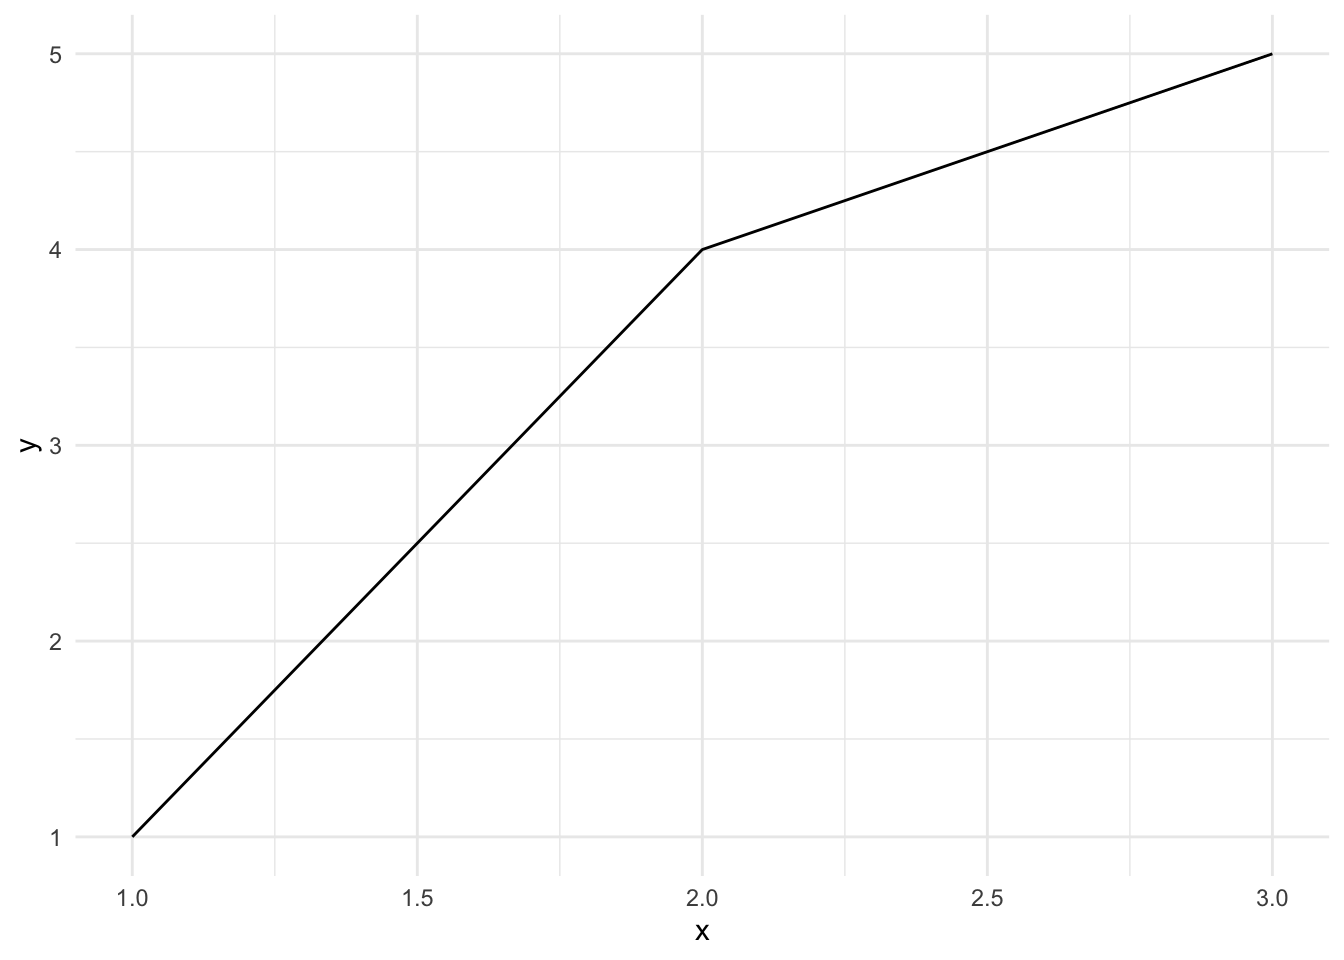
\includegraphics{intro_to_stats_files/figure-latex/unnamed-chunk-27-1.pdf}

but rather that the model can take into account more than one data axis (variable) (or dimension) - more like this, where a new variable is called \(z\), so the whole thing if plotted looks more like the top 3D panel here in which the model allows us to see the combined effects of \(x\) and \(z\) on the output \(y\) but we can focus on each variable individually by taking one at a time, like in the two split panels at the bottom (note how this is like looking into the front and right side of the 3D panel individually).

\begin{Shaded}
\begin{Highlighting}[]
\KeywordTok{its_three_variable_plot_time}\NormalTok{()}
\end{Highlighting}
\end{Shaded}

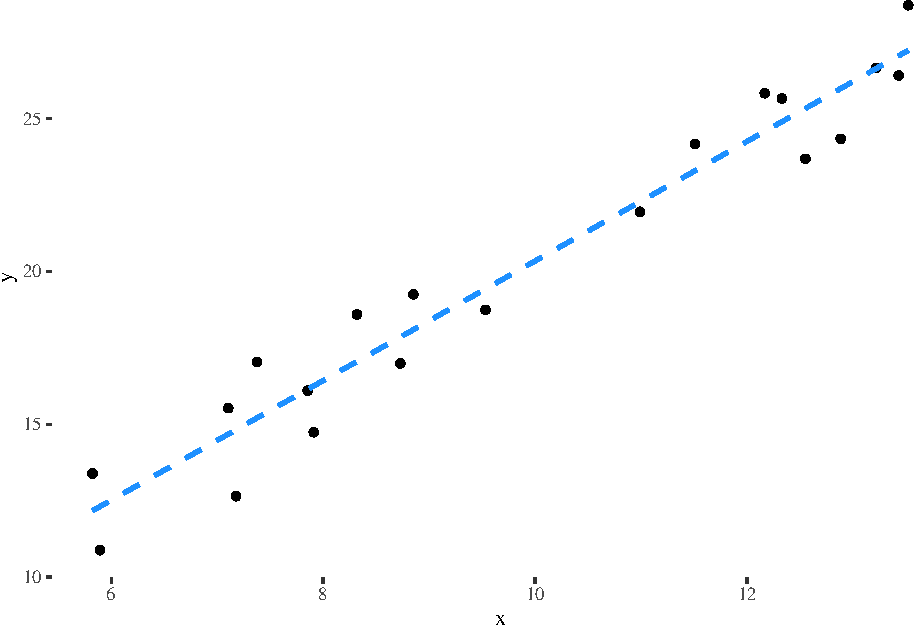
\includegraphics{intro_to_stats_files/figure-latex/unnamed-chunk-28-1.pdf}

We can only see up to two extra axes in a plot, and only visualise three without getting twitchy eyes, but going to three, four or many more dimensions is no problem for the linear model framework and they all work the same way. When it comes to notating this we run into a problem as we run out of letters. Let's build it up\ldots{}

First, a one slope/coefficient/independent variable model, adding one variable at a time

\begin{equation}
y = ax + e
\end{equation}

The first thing that happens is the linear model disposes of the intercept term \(b\), that's OK, it is still computed, but we don't have it in the model notation now. Next we build up the number of variables/dimensions. We've already used \(a\) and \(x\) so for the next slope we can use \(z\) for the variable and \(b\) for its coefficient. We can go further for a third slope and use \(w\) and \(c\)

\begin{align*}
y &= ax + bz + e\\
y &= ax + bz + cw + e
\end{align*}

Hold on though, this is already getting very confusing, \(cw\) is a bit hard to follow and it only gets worse. To get around this proliferation the notation of a linear model usually uses subscript numbers, all coefficients are given the Greek letter beta \(\beta\), all variables are given \(x\) and each is written with a little number after that distinguishes them

\begin{equation}
y = \beta_1 x_1 + e
\end{equation}

then that can be extended easily to \(n\) sets of variables. Finally, because the relationship between \(y\) and the variables in a linear model isn't strictly speaking a mathematical equality we use the \textasciitilde{} operator.

\begin{equation}
y \sim \beta_1 x_1 + \beta_2 x_2 \dotsc + \beta_n x_n + e
\end{equation}

We can see from this equation that a linear model is really just a load of variables added together to give some outcome \(y\). This makes much more sense when we put words in. Let's consider a plant growth experiment, in which we varied light, water and fertilizer and measured weight. The model in words looks like this

\begin{equation}
\mbox{weight} \sim \beta_1 \mbox{light} + \beta_2 \mbox{water} + \beta_3 \mbox{fertilizer} + e 
\end{equation}

We can see that what the linear model is looking for is all those values of \(\beta\) - it is going to calculate slopes for us. It is the job of the linear model to work out the coefficients and intercepts from the data we put into it and to tell us which of the slopes are non-zero ones and therefore important in determining the size of the output variable. With this information we can tell not only significant differences between the variables, but whether any are more important than others in affecting the outcome.

At the very least knowing notation like this will be useful later when we are looking at comparing multiple variables with linear models, but the linear model also gives us a lot of ways of talking about our experiment that we might not otherwise have had. The model gives us a way of assessing and quantifying the effects of the experimental variables on the outcome and a way of making quantitative predictions or hypotheses about the experiment, we can use expected values of the coefficients to say how we believe a model will work, when it proves to be different from the data we can validate or falsify our hypotheses.

\begin{roundup}
\begin{itemize}
\tightlist
\item
  Straight lines are described by an equation with two parameters

  \begin{itemize}
  \tightlist
  \item
    Linear models contain information about the data and can tell us whether a slope is likely flat or not given the data
  \end{itemize}
\end{itemize}
\end{roundup}

\hypertarget{r-fundamentals}{%
\chapter{R Fundamentals}\label{r-fundamentals}}

\hypertarget{about-this-chapter}{%
\section{About this chapter}\label{about-this-chapter}}

\begin{enumerate}
\def\labelenumi{\arabic{enumi}.}
\tightlist
\item
  Questions:
\end{enumerate}

\begin{itemize}
\tightlist
\item
  How do I use R?
\end{itemize}

\begin{enumerate}
\def\labelenumi{\arabic{enumi}.}
\setcounter{enumi}{1}
\tightlist
\item
  Objectives:
\end{enumerate}

\begin{itemize}
\tightlist
\item
  Become familiar with R syntax
\item
  Understand the concepts of objects and assignment
\item
  Get exposed to a few functions
\end{itemize}

\begin{enumerate}
\def\labelenumi{\arabic{enumi}.}
\setcounter{enumi}{2}
\tightlist
\item
  Keypoints:
\end{enumerate}

\begin{itemize}
\tightlist
\item
  R's capabilities are provided by functions
\item
  R users call functions and get results
\end{itemize}

\hypertarget{working-with-r}{%
\section{Working with R}\label{working-with-r}}

In this workshop we'll use R in the extremely useful RStudio software. For the most part we'll work interactively, meaning we'll type stuff straight into the R console in RStudio (Usually this is a window on the left or lower left) and get our results there too (usually in the console or in a window on the right).

Panels like the ones below mimic the interaction with R and first show the thing to type into R, and below the calculated result from R.

Let's look at how R works by using it for it's most basic job - as a calculator:

\begin{Shaded}
\begin{Highlighting}[]
 \DecValTok{3} \OperatorTok{+}\StringTok{ }\DecValTok{5}
\end{Highlighting}
\end{Shaded}

\begin{verbatim}
## [1] 8
\end{verbatim}

\begin{Shaded}
\begin{Highlighting}[]
 \DecValTok{12} \OperatorTok{*}\StringTok{ }\DecValTok{2}
\end{Highlighting}
\end{Shaded}

\begin{verbatim}
## [1] 24
\end{verbatim}

\begin{Shaded}
\begin{Highlighting}[]
 \DecValTok{1} \OperatorTok{/}\StringTok{ }\DecValTok{3}
\end{Highlighting}
\end{Shaded}

\begin{verbatim}
## [1] 0.3333333
\end{verbatim}

\begin{Shaded}
\begin{Highlighting}[]
 \DecValTok{12} \OperatorTok{*}\StringTok{ }\DecValTok{2}
\end{Highlighting}
\end{Shaded}

\begin{verbatim}
## [1] 24
\end{verbatim}

Fairly straightforward, we type in the expression and we get a result. That's how this whole book will work, you type the stuff in, and get answers out. It'll be easiest to learn if you go ahead and copy the examples one by one. Try to resist the urge to use copy and paste. Typing longhand really encourages you to look at what you're entering.

As far as the R output itself goes, it's really straightforward - its just the answer with a \texttt{{[}1{]}} stuck on the front. This \texttt{{[}1{]}} tells us how many items through the output we are. Often R will return long lists of numbers and it can be helpful to have this extra information.

\hypertarget{variables}{%
\section{Variables}\label{variables}}

We can save the output of operations for later use by giving it a name using the assignment symbol \texttt{\textless{}-}. Read this symbol as `gets', so \texttt{x\ \textless{}-\ 5} reads as `x gets 5'. These names are called variables, because the value they are associated with can change.

Let's give five a name, \texttt{x} then refer to the value 5 by it's name. We can then use the name in place of the value. In the jargon of computing we say we are assigning a value to a variable.

\begin{Shaded}
\begin{Highlighting}[]
\NormalTok{ x <-}\StringTok{ }\DecValTok{5}
\NormalTok{ x}
\end{Highlighting}
\end{Shaded}

\begin{verbatim}
## [1] 5
\end{verbatim}

\begin{Shaded}
\begin{Highlighting}[]
\NormalTok{ x }\OperatorTok{*}\StringTok{ }\DecValTok{2}
\end{Highlighting}
\end{Shaded}

\begin{verbatim}
## [1] 10
\end{verbatim}

\begin{Shaded}
\begin{Highlighting}[]
\NormalTok{y <-}\StringTok{ }\DecValTok{3}
\NormalTok{x }\OperatorTok{*}\StringTok{ }\NormalTok{y}
\end{Highlighting}
\end{Shaded}

\begin{verbatim}
## [1] 15
\end{verbatim}

This is of course of limited value with just numbers but is of great value when we have large datasets, as the whole thing can be referred to by the variable.

\hypertarget{using-objects-and-functions}{%
\subsection{Using objects and functions}\label{using-objects-and-functions}}

At the top level, R is a simple language with two types of thing: functions and objects. As a user you will use functions to do stuff, and get back objects as an answer. Functions are easy to spot, they are a name followed by a pair of brackets. A function like \texttt{mean()} is the function for calculating a mean. The options (or arguments) for the function go inside the brackets:

\begin{Shaded}
\begin{Highlighting}[]
\KeywordTok{sqrt}\NormalTok{(}\DecValTok{16}\NormalTok{)}
\end{Highlighting}
\end{Shaded}

\begin{verbatim}
## [1] 4
\end{verbatim}

Often the result from a function will be more complicated than a simple number object, often it will be a vector (simple list), like from the \texttt{rnorm()} function that returns lists of random numbers

\begin{Shaded}
\begin{Highlighting}[]
\KeywordTok{rnorm}\NormalTok{(}\DecValTok{100}\NormalTok{)}
\end{Highlighting}
\end{Shaded}

\begin{verbatim}
##   [1]  0.270232075 -0.112933852 -0.854887806 -1.033741090  0.222026624
##   [6] -1.079481969 -0.441373899  2.020634788  0.072856488  0.708817307
##  [11]  0.850509404 -1.486197129  0.920529800  0.148328802 -0.236867797
##  [16] -0.473236193 -0.669206104  1.358526687  1.412918017 -0.732773768
##  [21] -0.080551917  0.810196822  0.502587532  1.124022640 -0.171279790
##  [26]  0.118151334  0.869902623 -0.091936205  0.068898788 -1.682426754
##  [31]  1.116955546 -1.351357574 -0.537166518 -0.370113610  0.354012224
##  [36] -0.809825285 -0.179724629 -1.147659646  0.096242383  0.814700103
##  [41]  0.982940735  0.850843482  1.207347447 -1.433778349 -1.100945680
##  [46] -0.277042218 -0.641363270  0.856874779  0.313843454  1.222462079
##  [51] -1.126327533  0.236297412 -1.272369556  0.315682687  0.355610384
##  [56]  0.004052138  1.149194486 -0.496614335 -0.746796520 -1.282767236
##  [61] -1.031771673 -2.072046704 -0.426067161 -0.776975633 -0.181812198
##  [66] -0.862307391 -0.182541922  1.370695476  1.342718956 -1.151762060
##  [71]  0.748764659  1.522147956 -1.453019874  1.210757937 -0.909345650
##  [76]  1.200410172 -0.165416227 -0.494206517 -1.564569420 -0.354367785
##  [81] -1.021964796  1.191805557  0.229314222 -1.272579083  0.691872220
##  [86] -0.028754757 -1.103832089 -1.035274763  0.139952624  0.682728655
##  [91] -1.135559328  1.772544877 -0.093926303 -2.321188155  0.151039364
##  [96] -0.691147261  0.830428846  1.192598468  0.309910662 -1.549384356
\end{verbatim}

We can combine objects, variables and functions to do more complex stuff in R, here's how we get the mean of 100 random numbers.

\begin{Shaded}
\begin{Highlighting}[]
\NormalTok{numbers <-}\StringTok{ }\KeywordTok{rnorm}\NormalTok{(}\DecValTok{100}\NormalTok{)}
\KeywordTok{mean}\NormalTok{(numbers)}
\end{Highlighting}
\end{Shaded}

\begin{verbatim}
## [1] 0.06927728
\end{verbatim}

Here we created a vector object with \texttt{rnorm(100)} and assigned it to the variable \texttt{numbers}. We than used the \texttt{mean()} function, passing it the variable \texttt{numbers}. The \texttt{mean()} function returned the mean of the hundred random numbers.

\hypertarget{dataframes}{%
\section{Dataframes}\label{dataframes}}

One of the more common objects that R uses is a dataframe. The dataframe is a rectangular table-like object that contains data, think of it like a spreadsheet tab. Like the spreadsheet, the dataframe has rows and columns, the columns have names and the different columns can have different types of data in. Here's a little one

\begin{verbatim}
##   names age    score
## 1 Guido  24 45.60326
## 2 Marty  45 93.90205
## 3  Alan  11 80.16470
\end{verbatim}

Usually we get a dataframe by loading in data from an external source or as a result from functions, occasionally we'll want to hand make one, which can be done with various functions, \texttt{data.frame} being the most common.

\begin{Shaded}
\begin{Highlighting}[]
\KeywordTok{data.frame}\NormalTok{(}
  \DataTypeTok{names =} \KeywordTok{c}\NormalTok{(}\StringTok{"Guido"}\NormalTok{, }\StringTok{"Marty"}\NormalTok{, }\StringTok{"Alan"}\NormalTok{),}
  \DataTypeTok{age =} \KeywordTok{c}\NormalTok{(}\DecValTok{24}\NormalTok{,}\DecValTok{45}\NormalTok{,}\DecValTok{11}\NormalTok{),}
  \DataTypeTok{score =} \KeywordTok{runif}\NormalTok{(}\DecValTok{3}\NormalTok{) }\OperatorTok{*}\StringTok{ }\DecValTok{100}
\NormalTok{)}
\end{Highlighting}
\end{Shaded}

\hypertarget{packages}{%
\section{Packages}\label{packages}}

Many of the tools we use in will come in R packages, little nuggets of code that group related functions together. Installing new packages can be done using the \texttt{Packages} pane of RStudio or the \texttt{install.packages()} function. When we wish to use that code we use the \texttt{library()} function

\begin{Shaded}
\begin{Highlighting}[]
\KeywordTok{library}\NormalTok{(somepackage)}
\end{Highlighting}
\end{Shaded}

\hypertarget{using-r-help}{%
\section{Using R Help}\label{using-r-help}}

R provides a command, called \texttt{?} that will display the documentation for functions. For example \texttt{?mean} will display the help for the \texttt{mean()} function.

\begin{Shaded}
\begin{Highlighting}[]
\NormalTok{?mean}
\end{Highlighting}
\end{Shaded}

As in all programming languages the internal documentation in R is written with some assumption that the reader is familiar with the language. This can be a pain when you are starting out as the help will seem a bit obscure at times. Don't worry about this, usually the \texttt{Examples} section will give you a good idea of how to use the function and as your experience grows then the more things will make more sense.

\begin{roundup}
\begin{itemize}
\tightlist
\item
  R is an excellent and powerful statistical computing environment
\end{itemize}
\end{roundup}

\begin{task}
Use the interactive tutorial \texttt{r-start} in the package \texttt{itssl} to get to grips with R

At the R-Studio Console

\begin{enumerate}
\def\labelenumi{\arabic{enumi}.}
\tightlist
\item
  Type \texttt{library(learnr)} and press \texttt{Enter}
\item
  Type \texttt{library(itssl)} and press \texttt{Enter}
\item
  Type `run\_tutorial(``r-start'', ``itssl'') and follow the tutorial that pops up.
\end{enumerate}
\end{task}

\hypertarget{t-tests-and-linear-models}{%
\chapter{\texorpdfstring{\(t\)-tests and linear models}{t-tests and linear models}}\label{t-tests-and-linear-models}}

\begin{enumerate}
\def\labelenumi{\arabic{enumi}.}
\tightlist
\item
  Questions
\end{enumerate}

\begin{itemize}
\tightlist
\item
  How can we compare two samples using a linear model?
\end{itemize}

\begin{enumerate}
\def\labelenumi{\arabic{enumi}.}
\setcounter{enumi}{1}
\tightlist
\item
  Objectives
\end{enumerate}

\begin{itemize}
\tightlist
\item
  Learn how to set up some categoric \(x\) data in the \texttt{lm()} function
\item
  Understand how the coefficient relates to our conceptual slope
\item
  Understand how the \(t\) and \(p\) values of the linear model tell us about significance
\end{itemize}

\begin{enumerate}
\def\labelenumi{\arabic{enumi}.}
\setcounter{enumi}{2}
\tightlist
\item
  Keypoints
\end{enumerate}

\begin{itemize}
\tightlist
\item
  Using categoric \(x\) data is the same as using continuous \(x\) data
\item
  The \(p\) value of the coefficient tests the same thing as a \(t\)-test
\end{itemize}

In this section we'll look at how the linear model can be used as a conceptual tool to understand the sort of comparison a \(t\)-test does and as a straightforward way to perform a hypothesis test.

\hypertarget{recap}{%
\section{Recap}\label{recap}}

Because I like hammering this point home, Im going to recap two important points from our earlier work on linear models.

\begin{enumerate}
\def\labelenumi{\arabic{enumi}.}
\tightlist
\item
  The slope of the model is the important thing
\item
  `Significance' tests only test whether the difference between two things is `probably not 0'
\end{enumerate}

\hypertarget{the-slope-of-the-model-again}{%
\subsection{The slope of the model again}\label{the-slope-of-the-model-again}}

Recall the simplified linear model equation we developed

\begin{equation}
y = ax + b
\end{equation}

and that if we let the coefficient \(a = 0\), the effect of \(x\) disappears

\begin{equation}
y = 0 x + b\\
y = b
\end{equation}

So the logical conclusion is that if we have a coefficient that is non-zero, we have a relationship/effect of \(x\) on \(y\).

It is this property that lets us use the linear model to work out whether there is a significant difference between groups. That is to say we can use it as a \(t\)-test!

\hypertarget{using-two-different-samples-instead-of-a-continuous-x-variable}{%
\section{\texorpdfstring{Using two different samples instead of a continuous \(x\) variable}{Using two different samples instead of a continuous x variable}}\label{using-two-different-samples-instead-of-a-continuous-x-variable}}

The second we try to apply what we've learned with the linear model to a two-sample dataset we hit an apparent problem because we've learned how to make linear models from datasets with a continuous, numeric \(x\)-axis, but the data we have for a \(t\)-test has a very different two category look, something like these here:

\begin{Shaded}
\begin{Highlighting}[]
\KeywordTok{library}\NormalTok{(itssl)}

\NormalTok{continuous_x <-}\StringTok{ }\KeywordTok{its_random_xy_time}\NormalTok{(}\DecValTok{20}\NormalTok{)}
\KeywordTok{its_plot_xy_time}\NormalTok{(continuous_x)}

\NormalTok{categoric_x <-}\StringTok{ }\KeywordTok{its_bardata_time}\NormalTok{()}
\KeywordTok{its_barplot_time}\NormalTok{(categoric_x)}
\end{Highlighting}
\end{Shaded}

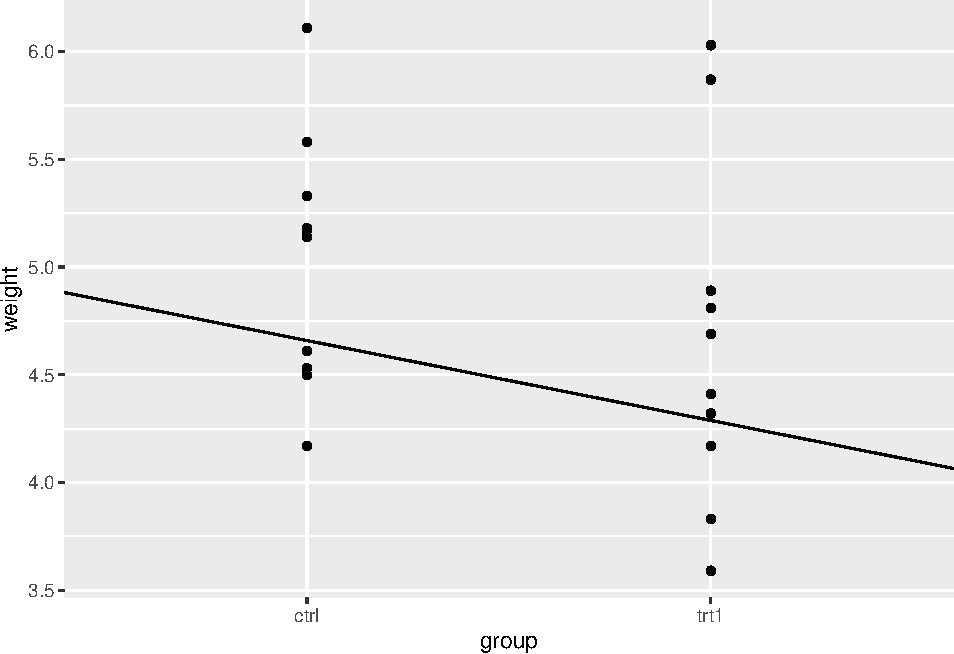
\includegraphics[width=0.5\linewidth]{intro_to_stats_files/figure-latex/unnamed-chunk-46-1} 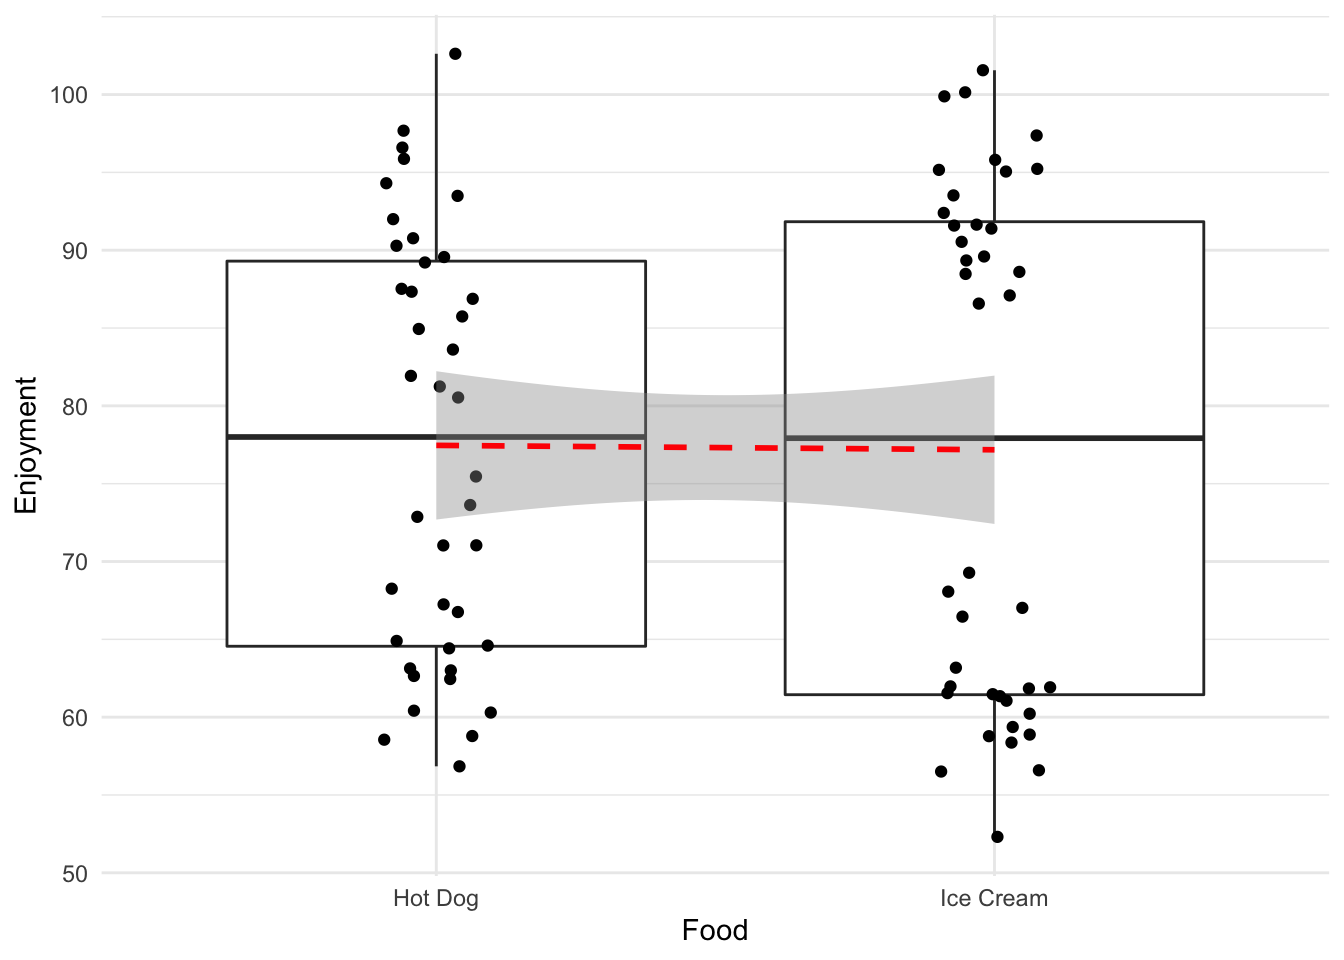
\includegraphics[width=0.5\linewidth]{intro_to_stats_files/figure-latex/unnamed-chunk-46-2}

Rest assured, the problem isn't insurmountable. We need to do a couple of numeric tricks to get this to work like the continuous data, and they're fairly easy, so let's run through them,

The first step is to realise that although we are used to thinking of the each of the bars representing a single number, that single number is (almost always) a summary, like a mean of replicate values, so let's go back to those source numbers as a first step and plot those, here are some examples

\begin{tabular}{c|c}
\hline
group1 & group2\\
\hline
4.895422 & 6.849330\\
\hline
5.225740 & 6.257527\\
\hline
4.828976 & 6.703222\\
\hline
5.878021 & 6.593268\\
\hline
4.068426 & 7.895864\\
\hline
4.985580 & 7.542633\\
\hline
\end{tabular}

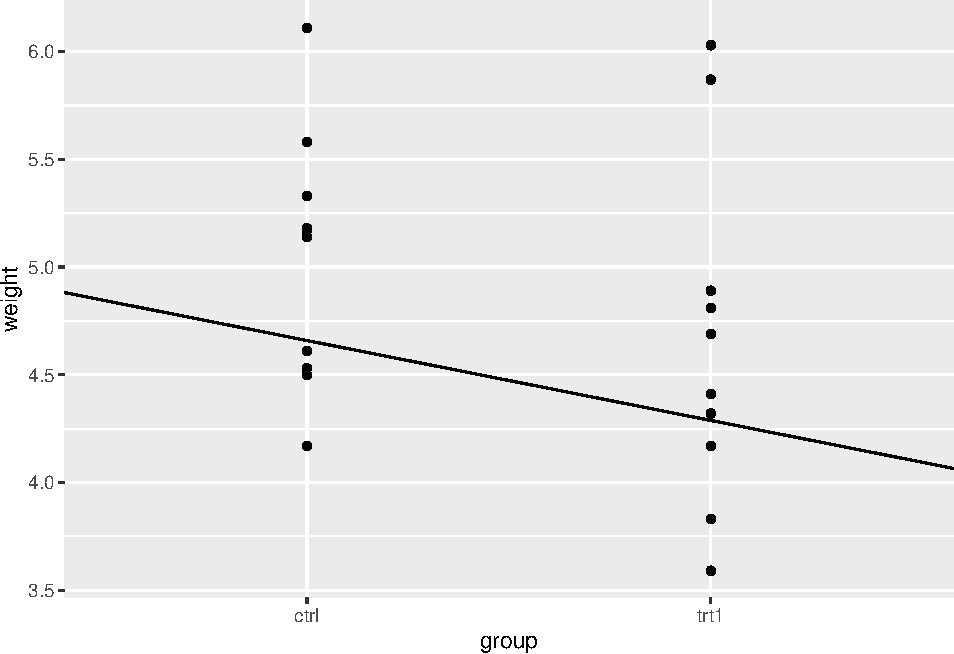
\includegraphics{intro_to_stats_files/figure-latex/unnamed-chunk-47-1.pdf}

plotting gives us something a lot more like the scatter plot we need for the model as we've been thinking about it, but it isn't quite clear how the categorical \(x\) becomes numeric. To do this we simply select a number for each group, so our data will look like this

\begin{Shaded}
\begin{Highlighting}[]
\KeywordTok{library}\NormalTok{(dplyr)}
\NormalTok{long_x <-}\StringTok{ }\KeywordTok{its_wide_to_long_time}\NormalTok{(categoric_x) }\OperatorTok\StringTok{ }
\StringTok{  }\KeywordTok{mutate}\NormalTok{(}\DataTypeTok{x =} \KeywordTok{if_else}\NormalTok{(group }\OperatorTok{==}\StringTok{ "group1"}\NormalTok{,}\DecValTok{0}\NormalTok{,}\DecValTok{1}\NormalTok{))}

\KeywordTok{its_table_time}\NormalTok{(long_x)}
\end{Highlighting}
\end{Shaded}

\begin{tabular}{c|c|c}
\hline
group & value & x\\
\hline
group1 & 4.895422 & 0\\
\hline
group2 & 6.849330 & 1\\
\hline
group1 & 5.225740 & 0\\
\hline
group2 & 6.257527 & 1\\
\hline
group1 & 4.828976 & 0\\
\hline
group2 & 6.703222 & 1\\
\hline
group1 & 5.878021 & 0\\
\hline
group2 & 6.593268 & 1\\
\hline
group1 & 4.068426 & 0\\
\hline
group2 & 7.895864 & 1\\
\hline
group1 & 4.985580 & 0\\
\hline
group2 & 7.542633 & 1\\
\hline
\end{tabular}

So now we can make a plot with two numeric axes, that looks a lot more like the one we're expecting for our model

\begin{Shaded}
\begin{Highlighting}[]
\KeywordTok{library}\NormalTok{(ggplot2)}
  \KeywordTok{ggplot}\NormalTok{(long_x) }\OperatorTok{+}\StringTok{ }\KeywordTok{aes}\NormalTok{(x, value) }\OperatorTok{+}\StringTok{ }\KeywordTok{geom_point}\NormalTok{() }\OperatorTok{+}\StringTok{ }\KeywordTok{theme_minimal}\NormalTok{() }
\end{Highlighting}
\end{Shaded}

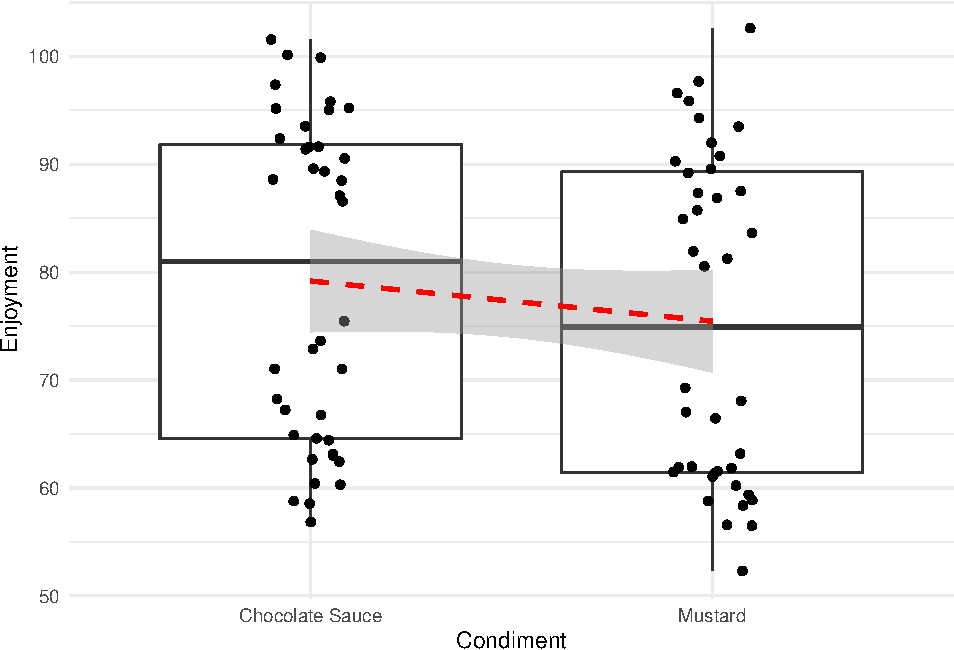
\includegraphics{intro_to_stats_files/figure-latex/unnamed-chunk-49-1.pdf}

albeit with the \(x\)-values in two places on the \(x\)-axis - its enough for us to make a slope on the line between the two groups and that means that we can use the linear model for the categoric data, as we did for the continuous.

If this seems like a bit of a `hack' then I'd agree. However, this is part of the numeric bookkeeping that we often have to do in statistics. Its not wrong and `hacks' are usually just pragmatic and useful solutions to problems, this one is completely mathematically legitimate as well as useful.

And if this change in the data reminds you of tidy data we've used in other courses, like dplyr, then that is no accident. Tidy data is designed to make this sort of analysis easy to work through, at least as far as organising the data goes.

The good news is that once we have our data set up with a category and value column, the \texttt{lm()} function just deals with assigning the numbers for us, we don't have to worry, the problem of continuous or categoric \(x\)-axes just disappears! All you need to know is that under the hood the linear model uses numbers for categories instead of words to make things easy.

Now that we understand how we can use categoric data in a linear model, let's get to the point of this chapter and work through an example of a linear model based hypothesis test for differences between two groups that functions as a \(t\)-test.

\hypertarget{the-plantgrowth-data}{%
\section{The PlantGrowth data}\label{the-plantgrowth-data}}

R comes with lots of datasets built in. One if these is \texttt{PlantGrowth}, which describes the dry weight of plants in grams in replicated measurements in a control and two treatments. We can load it with \texttt{data()} and get a \texttt{summary()}

\begin{Shaded}
\begin{Highlighting}[]
\KeywordTok{data}\NormalTok{(}\StringTok{"PlantGrowth"}\NormalTok{)}
\KeywordTok{summary}\NormalTok{(PlantGrowth)}
\end{Highlighting}
\end{Shaded}

\begin{verbatim}
##      weight       group   
##  Min.   :3.590   ctrl:10  
##  1st Qu.:4.550   trt1:10  
##  Median :5.155   trt2:10  
##  Mean   :5.073            
##  3rd Qu.:5.530            
##  Max.   :6.310
\end{verbatim}

\begin{Shaded}
\begin{Highlighting}[]
\KeywordTok{head}\NormalTok{(PlantGrowth)}
\end{Highlighting}
\end{Shaded}

\begin{verbatim}
##   weight group
## 1   4.17  ctrl
## 2   5.58  ctrl
## 3   5.18  ctrl
## 4   6.11  ctrl
## 5   4.50  ctrl
## 6   4.61  ctrl
\end{verbatim}

We have three groups and one measurement. The \(x\) values would come from the \texttt{group} column (and we now know that because it is categoric rather than continuous we needn't worry, the model functions will just do the conversion for us). And of course the \(y\) values would come from the \texttt{weight} column.

In linear modelling jargon, the \(x\) values are called the independent or explanatory variable, simply because this is the one we changed over the course of the experiment. The \(y\) values are called the dependent or response variables as this is the one that responds or changes according to the changes in the independent variable.

For simplicity at this stage we'll work with two groups only. Let's remove \texttt{trt2}.

\begin{Shaded}
\begin{Highlighting}[]
\NormalTok{two_groups <-}\StringTok{ }\KeywordTok{its_remove_a_group_time}\NormalTok{(PlantGrowth)}
\KeywordTok{summary}\NormalTok{(two_groups)}
\end{Highlighting}
\end{Shaded}

\begin{verbatim}
##      weight       group   
##  Min.   :3.590   ctrl:10  
##  1st Qu.:4.388   trt1:10  
##  Median :4.750            
##  Mean   :4.846            
##  3rd Qu.:5.218            
##  Max.   :6.110
\end{verbatim}

With that done, we can look at the categorical scatter plot.

\begin{Shaded}
\begin{Highlighting}[]
\KeywordTok{library}\NormalTok{(ggplot2)}
\NormalTok{p <-}\StringTok{ }\KeywordTok{ggplot}\NormalTok{(two_groups) }\OperatorTok{+}\StringTok{ }\KeywordTok{aes}\NormalTok{(group, weight) }\OperatorTok{+}\StringTok{ }\KeywordTok{geom_point}\NormalTok{()}
\NormalTok{p}
\end{Highlighting}
\end{Shaded}

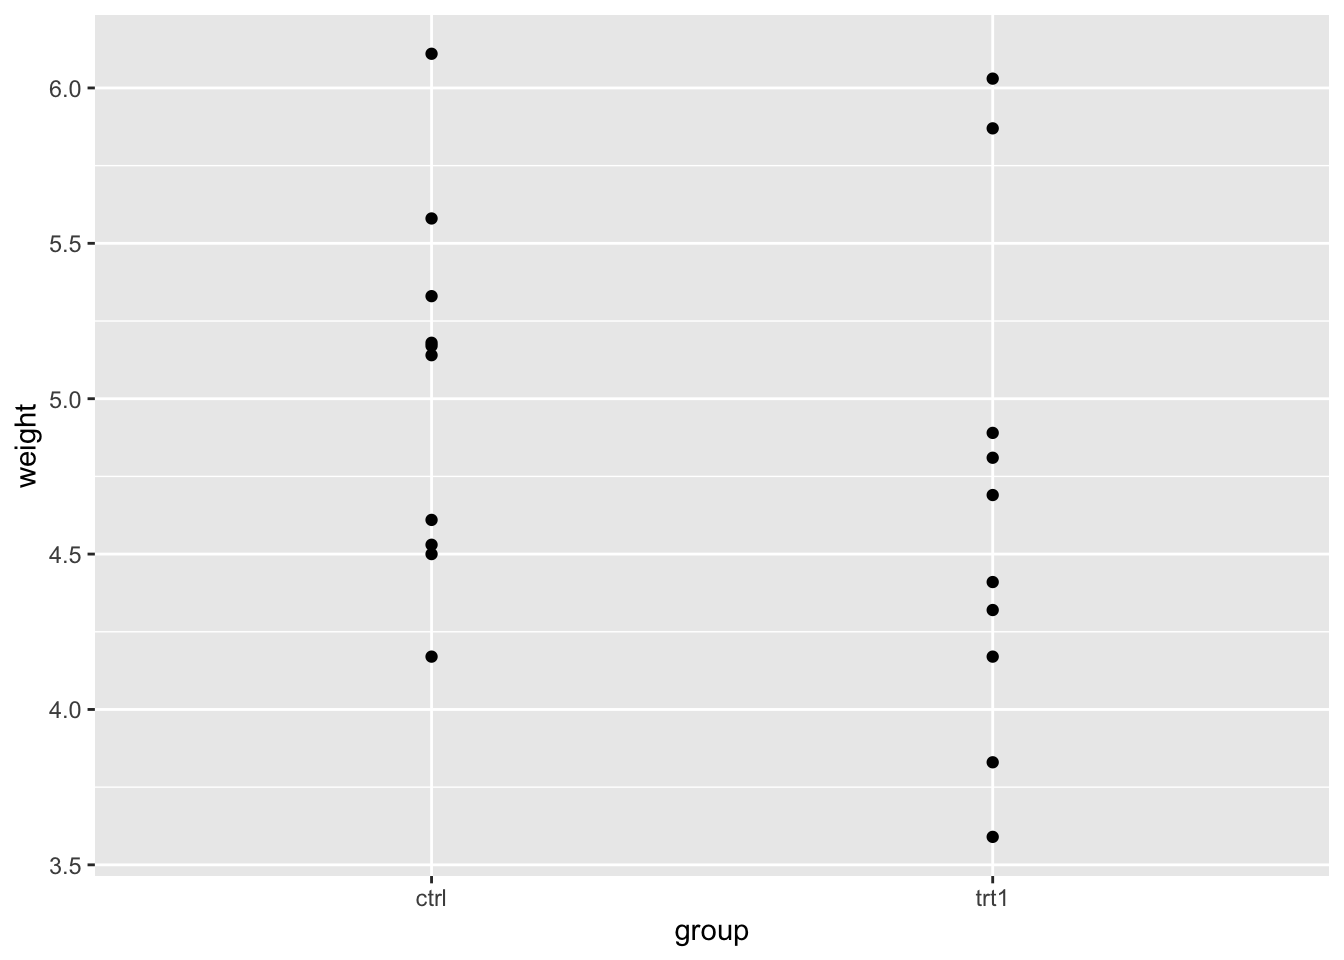
\includegraphics{intro_to_stats_files/figure-latex/unnamed-chunk-52-1.pdf}

We can clearly see the weight spread in each group. By eye we can see that the groups overlap in the \(y\)-axis (weight) quite considerably, though \texttt{trt1} seems to have a couple of data points that are lower.

\hypertarget{a-linear-model-with-a-categoric-x-axis}{%
\section{\texorpdfstring{A linear model with a categoric \(x\)-axis}{A linear model with a categoric x-axis}}\label{a-linear-model-with-a-categoric-x-axis}}

Let's make the linear model and get the intercept and coefficient of the line. This can be done with \texttt{lm()} as we did before.

\begin{Shaded}
\begin{Highlighting}[]
\NormalTok{two_groups_model <-}\StringTok{ }\KeywordTok{lm}\NormalTok{(weight }\OperatorTok{~}\StringTok{ }\NormalTok{group, }\DataTypeTok{data =}\NormalTok{ two_groups)}
\NormalTok{two_groups_model}
\end{Highlighting}
\end{Shaded}

\begin{verbatim}
## 
## Call:
## lm(formula = weight ~ group, data = two_groups)
## 
## Coefficients:
## (Intercept)    grouptrt1  
##       5.032       -0.371
\end{verbatim}

That calculates easily! The \texttt{lm()} isn't worried by the fact that one of our variables is categoric. It knows all the levels of the \texttt{group} variable and gives us the intercept and coefficient as it did before.

\hypertarget{using-the-statistics-of-the-linear-model-to-test-for-differences}{%
\section{Using the statistics of the linear model to test for differences}\label{using-the-statistics-of-the-linear-model-to-test-for-differences}}

Now we have a categoric linear model built we can start to look at how to use it to check for differences between the groups.

\begin{Shaded}
\begin{Highlighting}[]
\KeywordTok{summary}\NormalTok{(two_groups_model)}
\end{Highlighting}
\end{Shaded}

\begin{verbatim}
## 
## Call:
## lm(formula = weight ~ group, data = two_groups)
## 
## Residuals:
##     Min      1Q  Median      3Q     Max 
## -1.0710 -0.4938  0.0685  0.2462  1.3690 
## 
## Coefficients:
##             Estimate Std. Error t value Pr(>|t|)    
## (Intercept)   5.0320     0.2202  22.850 9.55e-15 ***
## grouptrt1    -0.3710     0.3114  -1.191    0.249    
## ---
## Signif. codes:  0 '***' 0.001 '**' 0.01 '*' 0.05 '.' 0.1 ' ' 1
## 
## Residual standard error: 0.6964 on 18 degrees of freedom
## Multiple R-squared:  0.07308,	Adjusted R-squared:  0.02158 
## F-statistic: 1.419 on 1 and 18 DF,  p-value: 0.249
\end{verbatim}

From the output we can see the coefficient isn't huge, only about 1/3 of a gram \emph{decrease} as we change along the \(x\) axis by one unit. Saying change along the axis by one unit in categoric axes sounds a bit strange, but in the categoric data it just means switching from one group to the next. Recall that we put one group at 0 and the second at 1 when we were doing the numeric `hack' above, the distance between the groups is defined as 1, so it all makes sense to say 'a change along the \(x\) by one unit. Lets add the line to the plot and have a look.

\begin{Shaded}
\begin{Highlighting}[]
\NormalTok{p }\OperatorTok{+}\StringTok{ }\KeywordTok{geom_abline}\NormalTok{(}\DataTypeTok{intercept =} \FloatTok{5.03}\NormalTok{, }\DataTypeTok{slope =} \FloatTok{-0.371}\NormalTok{)}
\end{Highlighting}
\end{Shaded}

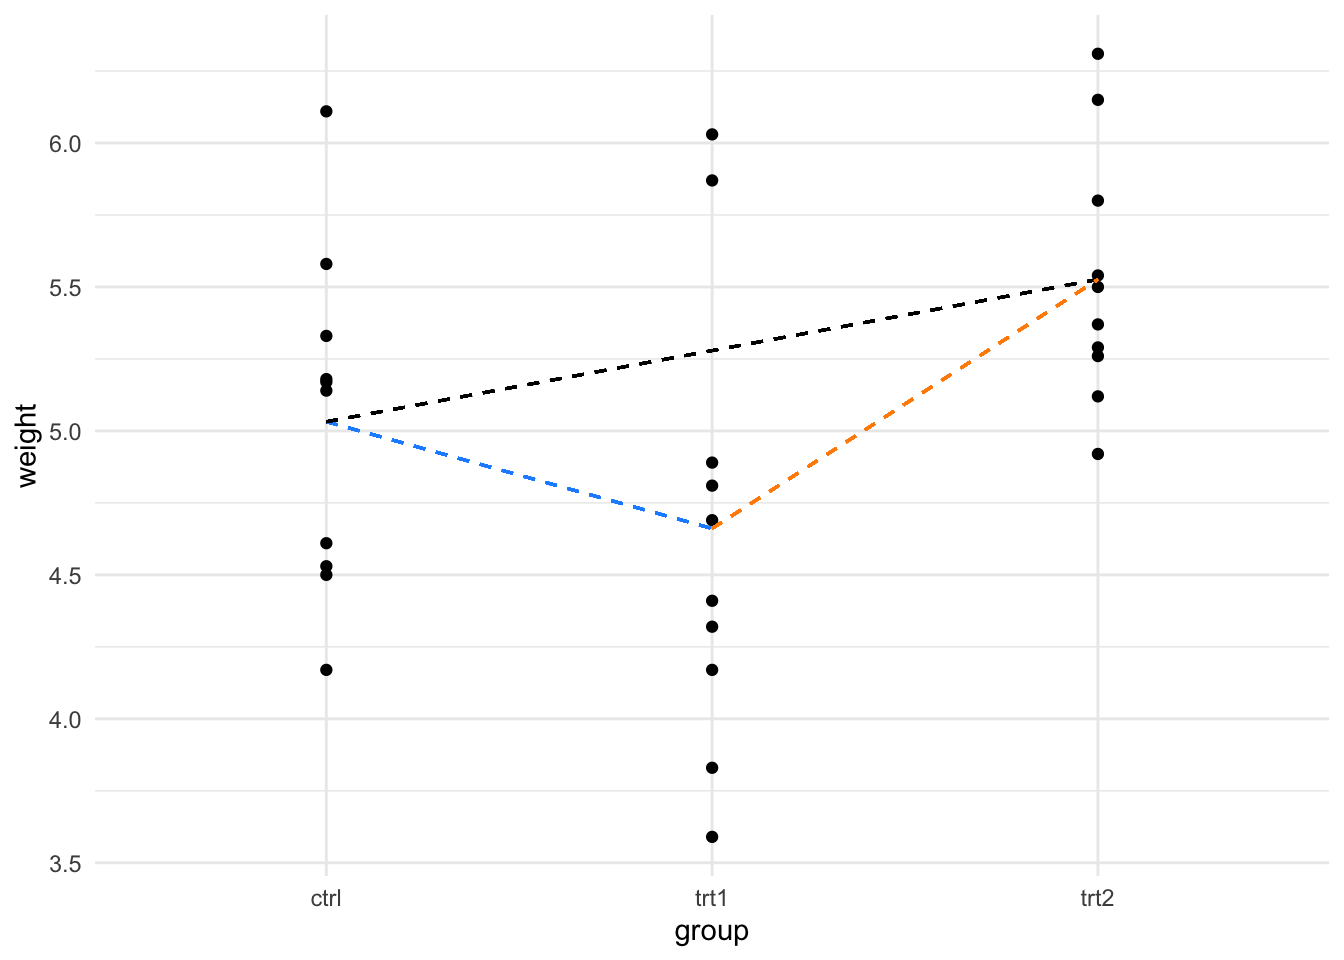
\includegraphics{intro_to_stats_files/figure-latex/unnamed-chunk-55-1.pdf}

Just looking at the plot makes the line seem more substantial than it is. Looking at the \(y\)-axis and the places where the line intercepts with the categories then we can see the difference is close to the coefficient.

\hypertarget{the-coefficient-and-the-mean-difference-between-groups-are-equivalent}{%
\subsection{The coefficient and the mean difference between groups are equivalent}\label{the-coefficient-and-the-mean-difference-between-groups-are-equivalent}}

Before we move along with our model, we should look at that coefficient of the group variable a bit more. As we're moving from the \texttt{ctrl} to \texttt{treatment} groups the coefficient tells us the size of the change. So does this mean that the coefficient is equivalent to other measures by which we can tell the difference in two groups - is it, for example equivalent to calculating the difference in the means of the groups? Short answer is yes! Let's look at that, recalling that the coefficient is \texttt{-0.371}.

First get the means of the groups using a little \texttt{dplyr}

\begin{Shaded}
\begin{Highlighting}[]
\NormalTok{mean_two_groups <-}\StringTok{ }\NormalTok{two_groups }\OperatorTok\StringTok{ }
\StringTok{  }\KeywordTok{group_by}\NormalTok{(group) }\OperatorTok\StringTok{ }
\StringTok{  }\KeywordTok{summarize}\NormalTok{(}\DataTypeTok{mean_wt =} \KeywordTok{mean}\NormalTok{(weight))}

\NormalTok{mean_two_groups}
\end{Highlighting}
\end{Shaded}

\begin{verbatim}
## # A tibble: 2 x 2
##   group mean_wt
##   <fct>   <dbl>
## 1 ctrl     5.03
## 2 trt1     4.66
\end{verbatim}

Now calculate the difference

\begin{Shaded}
\begin{Highlighting}[]
\FloatTok{5.03} \OperatorTok{-}\StringTok{ }\FloatTok{4.66}
\end{Highlighting}
\end{Shaded}

\begin{verbatim}
## [1] 0.37
\end{verbatim}

There you have it, the absolute values of each are very similar. You can use the coefficient as a way of finding the difference between the groups. Another handy feature of the linear model.

\hypertarget{the-p-value-of-the-co-efficient-tests-the-same-thing-as-a-t-test}{%
\subsection{\texorpdfstring{The \(p\)-value of the co-efficient tests the same thing as a \(t\)-test}{The p-value of the co-efficient tests the same thing as a t-test}}\label{the-p-value-of-the-co-efficient-tests-the-same-thing-as-a-t-test}}

We already know that the \(Pr(>|t|)\) value (\(p\)-value of the coefficient) tells us the probability that we would see the slope observed or greater in random samples if the real difference were 0. The two-sample \(t\)-test reports the probability that we would see the difference in means observed if the real difference were 0. So the two are very similar, the question is are they similar enough as a replacement?

The \(p\)-value for the coefficient in the linear model was 0.249. How does this compare with a \(t\)-test?

\begin{Shaded}
\begin{Highlighting}[]
\KeywordTok{t.test}\NormalTok{(weight }\OperatorTok{~}\StringTok{ }\NormalTok{group, }\DataTypeTok{data =}\NormalTok{ two_groups)}
\end{Highlighting}
\end{Shaded}

\begin{verbatim}
## 
## 	Welch Two Sample t-test
## 
## data:  weight by group
## t = 1.1913, df = 16.524, p-value = 0.2504
## alternative hypothesis: true difference in means is not equal to 0
## 95 percent confidence interval:
##  -0.2875162  1.0295162
## sample estimates:
## mean in group ctrl mean in group trt1 
##              5.032              4.661
\end{verbatim}

It is extremely close! In fact, as the sample size increases and gets over about 15 it gets to be exact. So this is useful, we can use the linear model slope and \(p\)-value as a mental and practical alternative for thinking about the more complicated to understand \(t\)-test. We can use the linear model \emph{instead} of the \(t\)-test if we want to.

All you have to understand is that you are looking at the slope of the line between the groups. If you don't see a slope of that size very often, then you can say its not likely that there's no difference \footnote{Again this is weak inference, but that's this type of statistics for you!}

\hypertarget{summary}{%
\section{Summary}\label{summary}}

Hopefully, this plot summarises how to look for differences between two groups using a linear model quite succinctly.

\begin{enumerate}
\def\labelenumi{\arabic{enumi}.}
\tightlist
\item
  Think of the line between the mean of the groups
\item
  Does the \(p\)-value tell you that you don't see a slope of this size often.
\end{enumerate}

So you just need the coefficient and the \(p\)-value from the linear model.
When we're thinking of the coefficient of the linear model for differences we're just asking something very similar to whether the line that joins the two means has a non-zero slope, given the error.

In a hypothesis test way, what we're asking amounts to the following two hypotheses:

\begin{itemize}
\tightlist
\item
  A flat line with slope of zero is equivalent to the Null hypothesis

  \begin{itemize}
  \tightlist
  \item
    \(H_{0}\) the group means are equal
  \end{itemize}
\item
  A \(p\)-value that suggests the slope is rare is equivalent to the Alternative hypothesis

  \begin{itemize}
  \tightlist
  \item
    \(H_{1}\) the group means are not equal
  \end{itemize}
\end{itemize}

and it can be summarised verbally as in this diagram

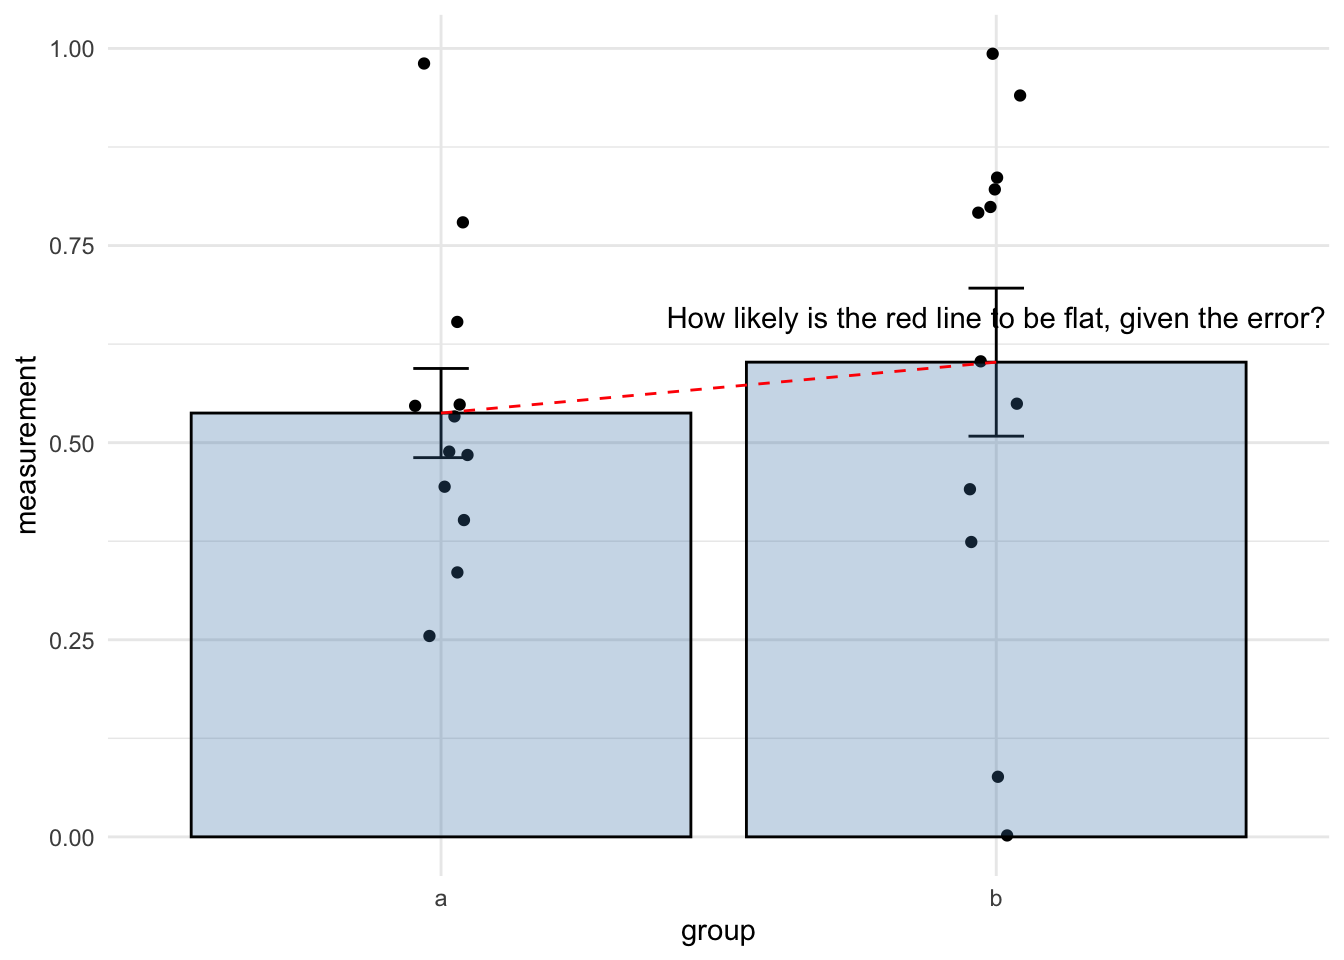
\includegraphics{intro_to_stats_files/figure-latex/unnamed-chunk-59-1.pdf}

\hypertarget{but-wasnt-the-t-test-just-easier}{%
\section{\texorpdfstring{But wasn't the \(t\)-test just easier?}{But wasn't the t-test just easier?}}\label{but-wasnt-the-t-test-just-easier}}

In the sloped line / linear model process we've been learning we used the \texttt{t.test()} function to calculate the \(p\)-value that tested the hypothesis that the true difference in the means between groups was 0. This was pretty easy and we didn't have to think too hard, we just got the result. Why wouldn't we stick to just using that, especially if it's equivalent to the linear model? There's no definitive reason, the \(t\)-test is a perfectly good tool, and it's a great one to use. Don't feel like I'm telling you not to use the \(t\)-test.

The focus of this whole tutorial is to give you a way to think of statistical techniques that is generally useful. Because the linear model provides a general answer to all these sorts of questions - one small set of techniques is re-usable lots of times, so the idea goes that in lots of experiments the statistics become a lot easier to understand. I hope I'm not confusing the two intents. If you've followed the logic of the straight line and slope and the linear model and can use it to inform your \(t\)-test usage in the future, then we're in good shape.

The general applicability of the straight line and linear model concept comes in handy when comparing more than two groups. Looking at effects in these experiments is basically the same thing as doing just two, though traditionally we'd use a seemingly very different sort of test - ANOVA. We'll look at that in the next section.

\begin{roundup}
\begin{itemize}
\tightlist
\item
  A linear model can be used as a \(t\)-test

  \begin{itemize}
  \tightlist
  \item
    Using the linear model rather than the \(t\)-test gives us a more consistent and flexible framework to think about differences between groups
  \end{itemize}
\end{itemize}
\end{roundup}

\begin{task}
Do th thing
\end{task}

\hypertarget{anova-and-linear-models}{%
\chapter{ANOVA and linear models}\label{anova-and-linear-models}}

\begin{enumerate}
\def\labelenumi{\arabic{enumi}.}
\tightlist
\item
  Questions
\end{enumerate}

\begin{itemize}
\tightlist
\item
  How can we compare many variables and factor levels
\item
  How can we check for interactions between treatments
\end{itemize}

\begin{enumerate}
\def\labelenumi{\arabic{enumi}.}
\setcounter{enumi}{1}
\tightlist
\item
  Objectives
\end{enumerate}

\begin{itemize}
\tightlist
\item
  Learn how to specify more complicated linear models
\item
  Understand how ANOVA works with a linear model
\item
  Understand how to spot interactions from plots
\item
  Learn how to deal with interactions in ANOVA
\end{itemize}

\begin{enumerate}
\def\labelenumi{\arabic{enumi}.}
\setcounter{enumi}{2}
\tightlist
\item
  Keypoints
\end{enumerate}

\begin{itemize}
\tightlist
\item
  Working with many variables is the same as working with just one
\item
  ANOVA is a tool for specifying comparisons between variables in linear models
\item
  We must take care to account for interactions between the variables
\end{itemize}

\hypertarget{comparing-groups-in-a-single-variable}{%
\section{Comparing groups in a single variable}\label{comparing-groups-in-a-single-variable}}

In the last section we looked at using the linear model to compare two groups, in this section we'll look at using it to compare more than two. One thing to note is that (for now) we're still working with only one explanatory variable, the groups we are talking about are basically different values that the one variable can take. In the \texttt{PlantGrowth} data the variable is called \texttt{group} and the values it takes are \texttt{ctrl}, \texttt{trt1} and \texttt{trt2}.

You'll be pleased to know this is where the pay off comes. Any number of groups (and later any number of variables) is no more complicated than the two we've already done.

We can visualise the process as simply being a case where we have more than one line to examine. Consider this figure, here we draw the categorical scatter plot and draw lines joining all the different group means that indicate the different comparisons we might choose to do with these data.

\begin{Shaded}
\begin{Highlighting}[]
\KeywordTok{library}\NormalTok{(itssl)}
\KeywordTok{its_multi_category_with_lines_time}\NormalTok{()}
\end{Highlighting}
\end{Shaded}

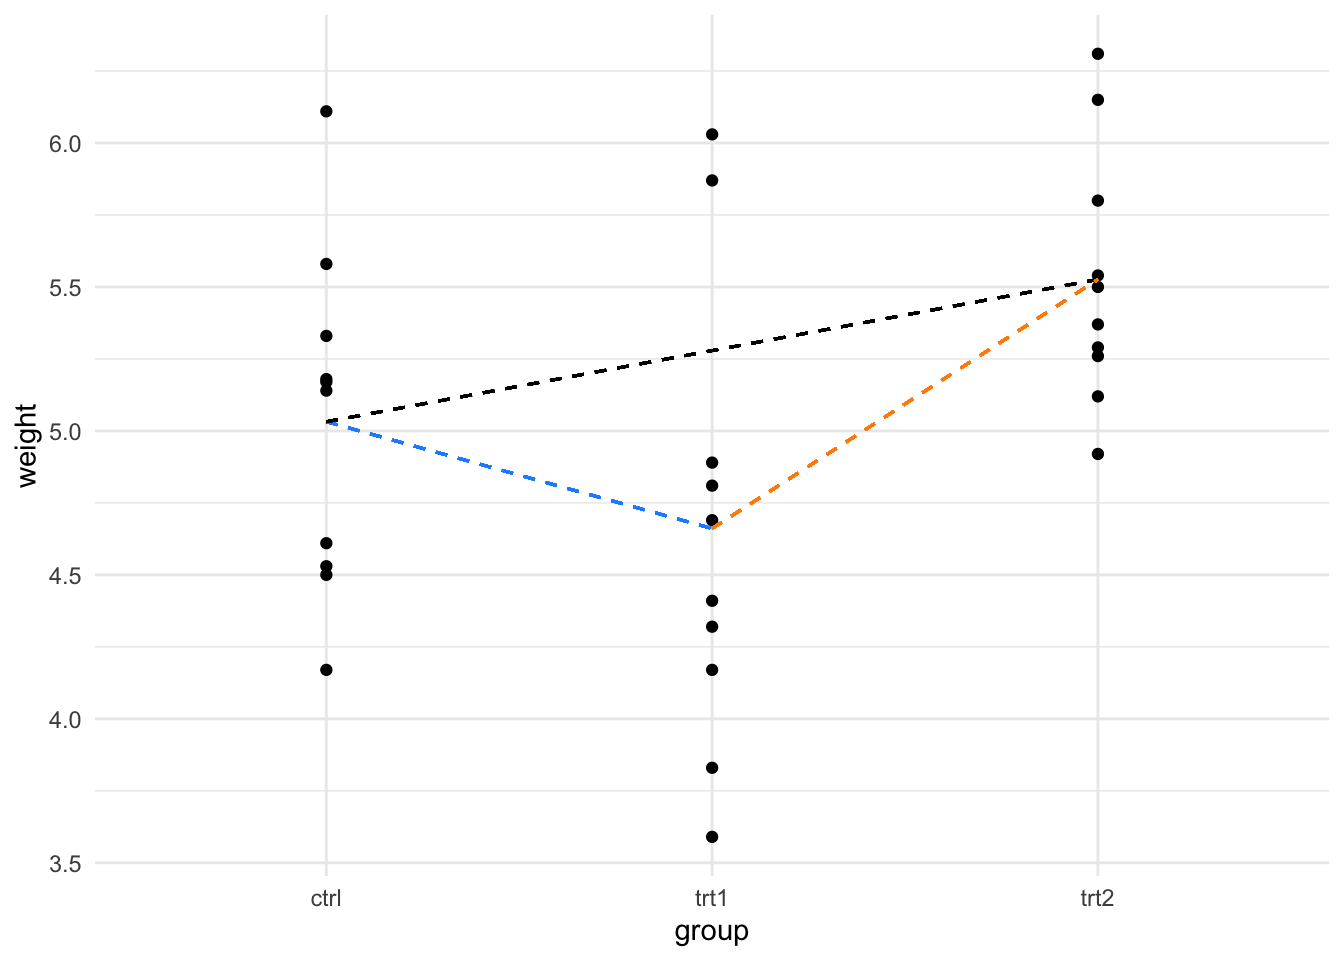
\includegraphics{intro_to_stats_files/figure-latex/unnamed-chunk-62-1.pdf}

So we'll need to know how to read the linear model for each of the given lines.
Let's jump in and work through that. First let's build a linear model with a variable with multiple groups.

\begin{Shaded}
\begin{Highlighting}[]
\NormalTok{model <-}\StringTok{ }\KeywordTok{lm}\NormalTok{(weight }\OperatorTok{~}\StringTok{ }\NormalTok{group, }\DataTypeTok{data =}\NormalTok{ PlantGrowth)}
\KeywordTok{summary}\NormalTok{(model)}
\end{Highlighting}
\end{Shaded}

\begin{verbatim}
## 
## Call:
## lm(formula = weight ~ group, data = PlantGrowth)
## 
## Residuals:
##     Min      1Q  Median      3Q     Max 
## -1.0710 -0.4180 -0.0060  0.2627  1.3690 
## 
## Coefficients:
##             Estimate Std. Error t value Pr(>|t|)    
## (Intercept)   5.0320     0.1971  25.527   <2e-16 ***
## grouptrt1    -0.3710     0.2788  -1.331   0.1944    
## grouptrt2     0.4940     0.2788   1.772   0.0877 .  
## ---
## Signif. codes:  0 '***' 0.001 '**' 0.01 '*' 0.05 '.' 0.1 ' ' 1
## 
## Residual standard error: 0.6234 on 27 degrees of freedom
## Multiple R-squared:  0.2641,	Adjusted R-squared:  0.2096 
## F-statistic: 4.846 on 2 and 27 DF,  p-value: 0.01591
\end{verbatim}

Great! so we handle the extra levels of the variable nearly perfectly. There are two lines of coefficient results, the first showing the gradient between the \texttt{ctrl} and \texttt{trt1} and the second showing the gradient between \texttt{ctrl} and \texttt{trt2}. The \texttt{ctrl} data has clearly been used as a common reference - this is the default design in the function, the first group in the data becomes the common reference. Here we get away with it, as we do want the first level to be the common reference. When you need to change the order, you can set the reference level explicitly.

\begin{Shaded}
\begin{Highlighting}[]
\NormalTok{df <-}\StringTok{ }\NormalTok{PlantGrowth}
\NormalTok{df}\OperatorTok{$}\NormalTok{group<-}\StringTok{ }\KeywordTok{relevel}\NormalTok{(df}\OperatorTok{$}\NormalTok{group, }\DataTypeTok{ref=}\StringTok{"trt2"}\NormalTok{)}
\NormalTok{model2 <-}\StringTok{ }\KeywordTok{lm}\NormalTok{(weight }\OperatorTok{~}\StringTok{ }\NormalTok{group  , }\DataTypeTok{data =}\NormalTok{ df,)}
\KeywordTok{summary}\NormalTok{(model2)}
\end{Highlighting}
\end{Shaded}

\begin{verbatim}
## 
## Call:
## lm(formula = weight ~ group, data = df)
## 
## Residuals:
##     Min      1Q  Median      3Q     Max 
## -1.0710 -0.4180 -0.0060  0.2627  1.3690 
## 
## Coefficients:
##             Estimate Std. Error t value Pr(>|t|)    
## (Intercept)   5.5260     0.1971  28.032  < 2e-16 ***
## groupctrl    -0.4940     0.2788  -1.772  0.08768 .  
## grouptrt1    -0.8650     0.2788  -3.103  0.00446 ** 
## ---
## Signif. codes:  0 '***' 0.001 '**' 0.01 '*' 0.05 '.' 0.1 ' ' 1
## 
## Residual standard error: 0.6234 on 27 degrees of freedom
## Multiple R-squared:  0.2641,	Adjusted R-squared:  0.2096 
## F-statistic: 4.846 on 2 and 27 DF,  p-value: 0.01591
\end{verbatim}

And now we see the \texttt{trt2} as common reference against the \texttt{ctrl} and \texttt{trt1} groups.

In these data only \texttt{trt2\ vs\ trt1} appears to be significant according to the linear model \texttt{model2} but we did need to create two models to do this, which is a bit of a statistical mess. If this seems longwinded or illogical, then that's fair. The two models have the same data and specification so should have the same results in - it was really just the way we were ordering things in the data that was different. The real problem is just one of bookkeeping.

The linear models are rich and not all the comparisons that can be done with them can easily be written in \texttt{summary(model)}. To answer specific questions from an analysis technique for getting specific comparisons (or contrasts in the statistics jargon) from linear models has been invented, that technique is called ANOVA (Analysis of Variance).

\begin{sidenote}
I know, I gave you the impression that we would be using linear models and not ANOVAs, but the thing is, ANOVAs have always been based on linear models. In a way ANOVA isn't a test of its own, not in the way we think of \(t\)-tests or \(\chi\)-squared tests. ANOVA is plural, they are a set of tools for pulling comparisons straight out of linear models in the best way. So that's another great reason for having bothered to understand something of how linear models work.
\end{sidenote}

\hypertarget{one-way-comparisons---groups-in-a-single-variable}{%
\section{One-Way comparisons - groups in a single variable}\label{one-way-comparisons---groups-in-a-single-variable}}

The situation where we have just one variable is called a `One-Way' ANOVA.

Now that we have a solid way of thinking about contrasts as the slope between the categories, we can think of ANOVA as a tool for pulling out the significances in the best way. All we have to do is learn how to specify the contrasts for ANOVA.

Every time we do ANOVA we need a model to feed into it. Here's the most common way ANOVA is done in R, with the \texttt{aov()} and \texttt{TukeyHSD()} functions, you've probably seen this before.

\begin{Shaded}
\begin{Highlighting}[]
\NormalTok{ano <-}\StringTok{ }\KeywordTok{aov}\NormalTok{(model)}
\KeywordTok{TukeyHSD}\NormalTok{(ano)}
\end{Highlighting}
\end{Shaded}

\begin{verbatim}
##   Tukey multiple comparisons of means
##     95% family-wise confidence level
## 
## Fit: aov(formula = model)
## 
## $group
##             diff        lwr       upr     p adj
## trt1-ctrl -0.371 -1.0622161 0.3202161 0.3908711
## trt2-ctrl  0.494 -0.1972161 1.1852161 0.1979960
## trt2-trt1  0.865  0.1737839 1.5562161 0.0120064
\end{verbatim}

It seems to do the job, though the `flavour' of ANOVA it does is sometimes limited and applies only when the standard assumptions of ANOVA are met.

\begin{sidenote}
A scary thing that statisticians often say is that such-and-such a method is only applicable when certain assumptions are met. This can make scientists nervy about applying any methods in case it is wrong. I would like to encourage you to relax about this aspect. Most statistical tests are pretty robust to against violations, and if anything tend to get more conservative (IE, generate fewer significant results) in these cases. There are a few assumptions and even a few types of data that we need to be aware of. I dedicate some space in the last chapter to understanding where these trip-ups might happen.
\end{sidenote}

A better alternative than the quick and dirty ANOVA approach above (in the sense of flexibility for the user) is the \texttt{multcomp} package function \texttt{glht()} (general linear model hypothesis test), which is more flexible with respect to which designs and contrasts you can get out, at the expense of being a little more complicated. The basic case is straightforward though.

\begin{Shaded}
\begin{Highlighting}[]
\KeywordTok{library}\NormalTok{(multcomp)}
\NormalTok{tested <-}\StringTok{ }\KeywordTok{glht}\NormalTok{(model, }\DataTypeTok{linfct =} \KeywordTok{mcp}\NormalTok{(}\DataTypeTok{group =} \StringTok{"Tukey"}\NormalTok{))}
\KeywordTok{summary}\NormalTok{(tested)}
\end{Highlighting}
\end{Shaded}

\begin{verbatim}
## 
## 	 Simultaneous Tests for General Linear Hypotheses
## 
## Multiple Comparisons of Means: Tukey Contrasts
## 
## 
## Fit: lm(formula = weight ~ group, data = PlantGrowth)
## 
## Linear Hypotheses:
##                  Estimate Std. Error t value Pr(>|t|)  
## trt1 - ctrl == 0  -0.3710     0.2788  -1.331    0.391  
## trt2 - ctrl == 0   0.4940     0.2788   1.772    0.198  
## trt2 - trt1 == 0   0.8650     0.2788   3.103    0.012 *
## ---
## Signif. codes:  0 '***' 0.001 '**' 0.01 '*' 0.05 '.' 0.1 ' ' 1
## (Adjusted p values reported -- single-step method)
\end{verbatim}

The \texttt{linfct} option just takes a specification of the things to be tested, and the \texttt{mcp()} function is a helper that generates the comparison based on a text description, here that the variable \texttt{group} should be analysed by `Tukey'.

By printing the summary we see the contrast hypotheses writ explicitly (e.g.~the difference between \texttt{ctrl} and \texttt{trt1} is 0) and the conclusions: there is no evidence to suggest either treatment is different from the control, but the difference we observe between the \texttt{trt1} and \texttt{trt2} occurs by chance only about 1.2 percent of the time, so is deemed `significant'.

And that's it! A properly done and specified use of the linear model and a subsequent ANOVA with Tukey's \emph{post hoc} used to determine differences.

We'll see more of how to use \texttt{glht()} as we go.

\hypertarget{two-way-comparisons---groups-in-multiple-variables}{%
\section{Two-Way comparisons - groups in multiple variables}\label{two-way-comparisons---groups-in-multiple-variables}}

Often we'll have experimental data where we have more than one explanatory variable, for example, \texttt{compost} and \texttt{fertiliser} and want to know the effects of each on a response variable like \texttt{yield}. Where you have two variables, it's called a Two-Way ANOVA.

Two-Way comparisons are pretty similar in practice to One-Way comparisons. So similar in fact that you're going to jump in and try one, without any further instruction

\begin{task}
\begin{enumerate}
\def\labelenumi{\arabic{enumi}.}
\tightlist
\item
  Use the function \texttt{its\_compost\_time()} to load some data on the effects of changing compost type and a supplement on plant size.
\item
  Build a linear model specifying that size is related to the two other explanatory variables. We haven't explicitly discussed the syntax for two variables, but in the linear model a extra variables is added with `+', thats how its done in R e.g.~\texttt{lm(y\ \textasciitilde{}\ a\ +\ b\ +\ c)}. Inspect the model.
\item
  Carry out Tukey's to test the hypotheses i) that the true difference in means between Formula X1 and X2 is 0, and ii) that the true difference in means between John Innes \#1 and \#2 is 0.
\end{enumerate}
\end{task}

\hypertarget{interactions-between-variables}{%
\section{Interactions between variables}\label{interactions-between-variables}}

Working with multiple variables is complicated over the single case as we have the possibility of an interaction between the variables to consider. That is to say that the response in an experiment may be stronger under conditions \texttt{a\ and\ b} than in \texttt{a} or \texttt{b} alone whether \texttt{a} or \texttt{b} alone is greater than a \texttt{control} or not. We can visualise this as straight lines like in the diagrams below.

\begin{Shaded}
\begin{Highlighting}[]
\KeywordTok{its_interaction_example_time}\NormalTok{()}
\end{Highlighting}
\end{Shaded}

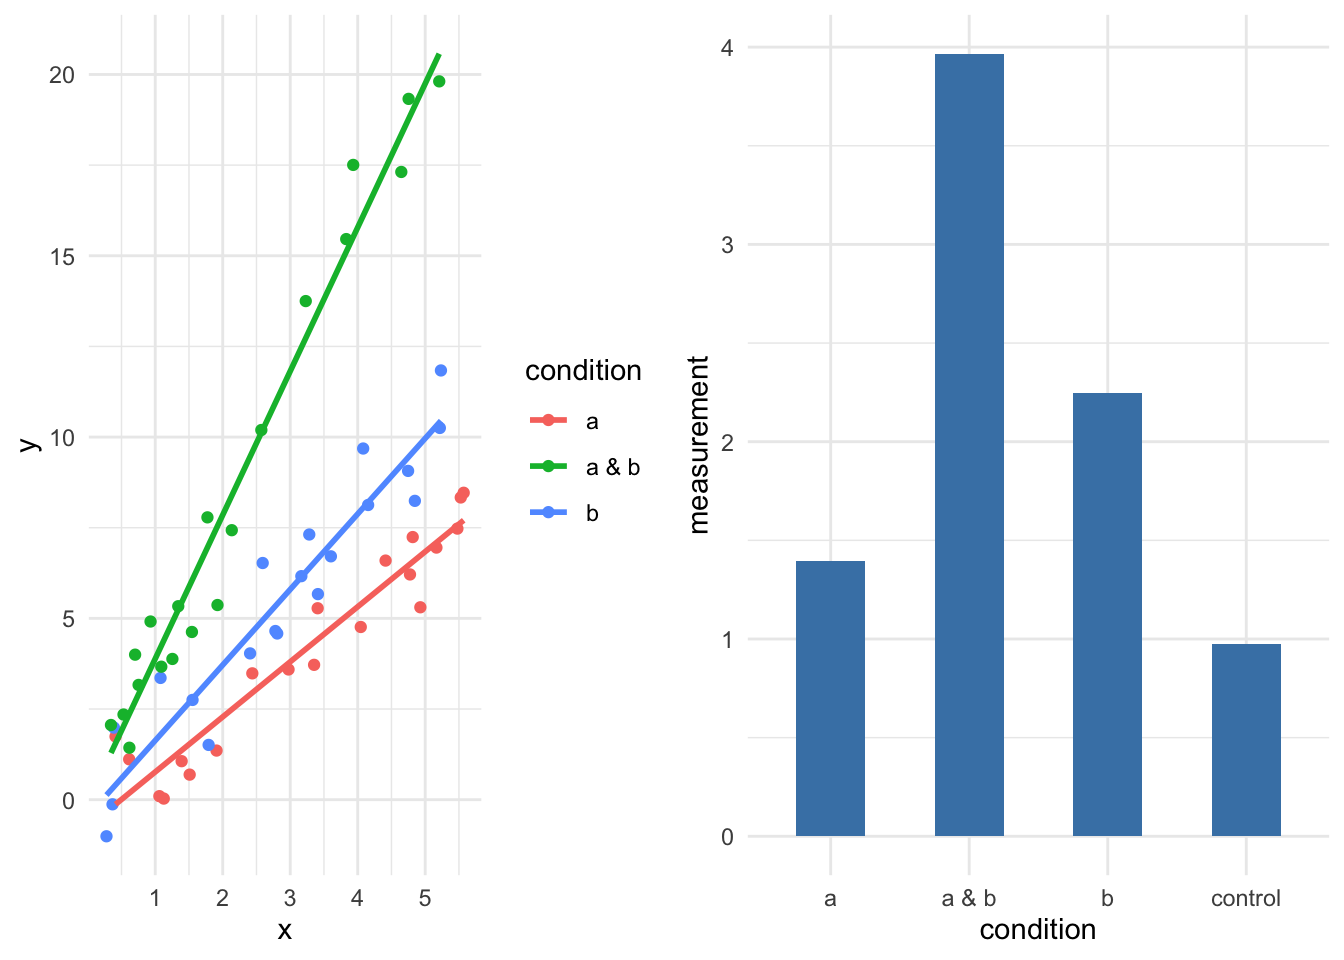
\includegraphics{intro_to_stats_files/figure-latex/unnamed-chunk-71-1.pdf}

We can see the effect of interaction quite clearly in the two types of data, whenever \texttt{a\ \&\ b} is used then we have greater responses, either in greater means or in steeper gradients.

Let's work through an example that highlights how we identify and investigate this with linear models and ANOVAs. Here's some data on reported enjoyment of some food, with different condiments added

\begin{Shaded}
\begin{Highlighting}[]
\NormalTok{food <-}\StringTok{ }\KeywordTok{its_food_data_time}\NormalTok{()}
\CommentTok{#look at specific rows 1,21,41,61}
\NormalTok{food[}\KeywordTok{c}\NormalTok{(}\DecValTok{1}\NormalTok{,}\DecValTok{21}\NormalTok{,}\DecValTok{41}\NormalTok{,}\DecValTok{61}\NormalTok{),]                                      }
\end{Highlighting}
\end{Shaded}

\begin{verbatim}
##              Food Condiment Enjoyment
## 1  Tortilla Chips   Hummous  87.19762
## 21 Tortilla Chips       Jam  55.72871
## 41       Porridge   Hummous  57.22117
## 61       Porridge       Jam  91.89820
\end{verbatim}

Looking at those in the way we have already - each variable individually - then we would generate the following plots and lines to examine.

\begin{Shaded}
\begin{Highlighting}[]
\KeywordTok{its_food_plot_time}\NormalTok{()}
\end{Highlighting}
\end{Shaded}

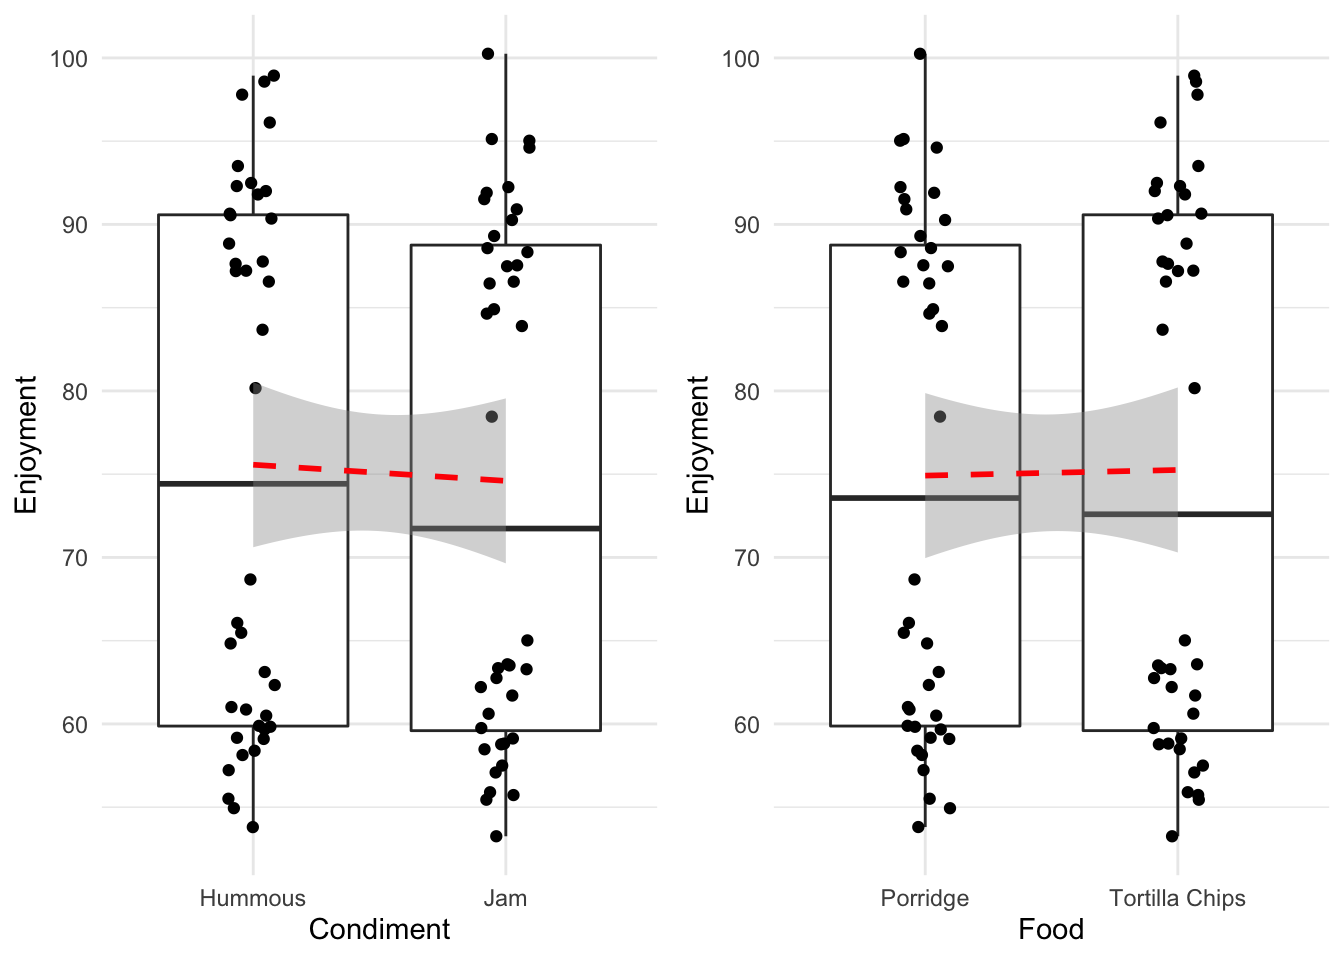
\includegraphics{intro_to_stats_files/figure-latex/unnamed-chunk-72-1.pdf}

Without rushing ahead to do the modelling, we see that hummous has a slightly greater effect on enjoyment than jam, whereas the enjoyment of the two food types is much more similar. So without a hypothesis test the dangerously thin conclusion would be `use hummous to enhance your enjoyment of Porridge or Tortilla Chips'. We might be suspect of this conclusion not only because it seems not to line up with our intuitive sense of what's going on, but also because of those strange splits in the data. Look within each column and you can see that there is a definite clustering that is not a good sign, we possibly don't have a good specification of our data here.

Let's see what the model says, in specifying the second variable can be added with a \texttt{+} as

\begin{Shaded}
\begin{Highlighting}[]
\NormalTok{model_}\DecValTok{1}\NormalTok{ <-}\StringTok{ }\KeywordTok{lm}\NormalTok{(Enjoyment }\OperatorTok{~}\StringTok{ }\NormalTok{Food }\OperatorTok{+}\StringTok{ }\NormalTok{Condiment, }\DataTypeTok{data =}\NormalTok{ food)}
\KeywordTok{summary}\NormalTok{(model_}\DecValTok{1}\NormalTok{)}
\end{Highlighting}
\end{Shaded}

\begin{verbatim}
## 
## Call:
## lm(formula = Enjoyment ~ Food + Condiment, data = food)
## 
## Residuals:
##     Min      1Q  Median      3Q     Max 
## -21.593 -15.526  -1.348  14.832  25.822 
## 
## Coefficients:
##                    Estimate Std. Error t value Pr(>|t|)    
## (Intercept)         75.3978     3.0674  24.580   <2e-16 ***
## FoodTortilla Chips   0.3384     3.5419   0.096    0.924    
## CondimentJam        -0.9693     3.5419  -0.274    0.785    
## ---
## Signif. codes:  0 '***' 0.001 '**' 0.01 '*' 0.05 '.' 0.1 ' ' 1
## 
## Residual standard error: 15.84 on 77 degrees of freedom
## Multiple R-squared:  0.00109,	Adjusted R-squared:  -0.02486 
## F-statistic: 0.04201 on 2 and 77 DF,  p-value: 0.9589
\end{verbatim}

The summary isn't promising, it looks like neither is significant. Let's do the ANOVA and get a clearer view.

The call to \texttt{glht()} is a bit more complicated than before, but not much

\begin{Shaded}
\begin{Highlighting}[]
\KeywordTok{summary}\NormalTok{(}\KeywordTok{glht}\NormalTok{(model_}\DecValTok{1}\NormalTok{, }\DataTypeTok{linfct =} \KeywordTok{mcp}\NormalTok{(}\DataTypeTok{Food =} \StringTok{"Tukey"}\NormalTok{, }\DataTypeTok{Condiment =} \StringTok{"Tukey"}\NormalTok{) ) )}
\end{Highlighting}
\end{Shaded}

\begin{verbatim}
## 
## 	 Simultaneous Tests for General Linear Hypotheses
## 
## Multiple Comparisons of Means: Tukey Contrasts
## 
## 
## Fit: lm(formula = Enjoyment ~ Food + Condiment, data = food)
## 
## Linear Hypotheses:
##                                      Estimate Std. Error t value Pr(>|t|)
## Food: Tortilla Chips - Porridge == 0   0.3384     3.5419   0.096    0.994
## Condiment: Jam - Hummous == 0         -0.9693     3.5419  -0.274    0.954
## (Adjusted p values reported -- single-step method)
\end{verbatim}

Neither factor seems to be significant. Hmm. This seems like a slightly strange conclusion - and it is. The presence of two variables is confusing this approach. Look at what we get if we split the data by the two variables at once.

\begin{Shaded}
\begin{Highlighting}[]
\KeywordTok{its_food_two_ways_time}\NormalTok{()}
\end{Highlighting}
\end{Shaded}

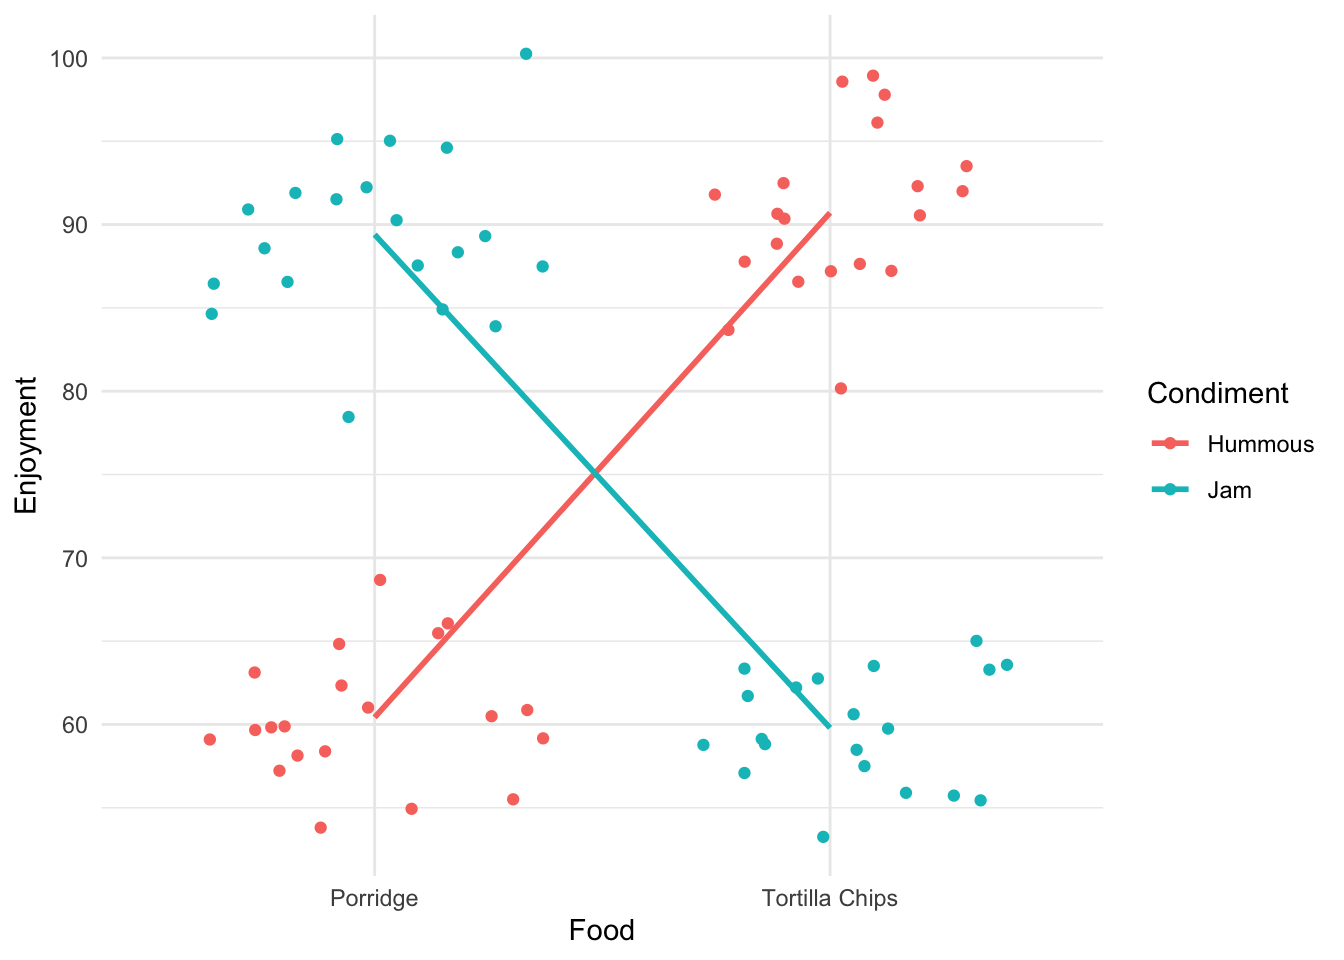
\includegraphics{intro_to_stats_files/figure-latex/unnamed-chunk-75-1.pdf}

Ok! That's very different and very much clearer. The enjoyment is very much dependent on the combination of food and condiment. This is a classic case of interaction between variables. You get results that are conditional on the combined values of the variables.

\begin{sidenote}
The cross-over of the lines is a visual diagnostic of the presence of an interaction effect.
\end{sidenote}

\hypertarget{analysing-and-modelling-an-interaction-effect}{%
\subsection{Analysing and modelling an interaction effect}\label{analysing-and-modelling-an-interaction-effect}}

The interaction effect should be checked for in the linear model. It is quite easy to check for and requires a slight extension to syntax. An interaction term can be specified with the \texttt{:}.

\begin{Shaded}
\begin{Highlighting}[]
\NormalTok{interaction_model <-}\StringTok{ }\KeywordTok{lm}\NormalTok{(Enjoyment }\OperatorTok{~}\StringTok{ }\NormalTok{Food }\OperatorTok{+}\StringTok{ }\NormalTok{Condiment }\OperatorTok{+}\StringTok{ }\NormalTok{Food}\OperatorTok{:}\NormalTok{Condiment, }\DataTypeTok{data =}\NormalTok{ food)}
\end{Highlighting}
\end{Shaded}

(there is also a short hand that allows the whole thing to be specified in one term \texttt{*}, which is used like \texttt{lm(Enjoyment\ \textasciitilde{}\ Food\ *\ Condiment,\ data=food)})

and when we print the \texttt{summary()} we get the book-keeping issue of not all the results we want to see being immediately available, but we can see the usual stuff.

\begin{Shaded}
\begin{Highlighting}[]
\KeywordTok{summary}\NormalTok{(interaction_model)}
\end{Highlighting}
\end{Shaded}

\begin{verbatim}
## 
## Call:
## lm(formula = Enjoyment ~ Food + Condiment + Food:Condiment, data = food)
## 
## Residuals:
##      Min       1Q   Median       3Q      Max 
## -10.9463  -2.8645  -0.2551   2.7201  10.8500 
## 
## Coefficients:
##                                 Estimate Std. Error t value Pr(>|t|)    
## (Intercept)                      60.4259     0.9553   63.25   <2e-16 ***
## FoodTortilla Chips               30.2822     1.3510   22.41   <2e-16 ***
## CondimentJam                     28.9745     1.3510   21.45   <2e-16 ***
## FoodTortilla Chips:CondimentJam -59.8876     1.9106  -31.34   <2e-16 ***
## ---
## Signif. codes:  0 '***' 0.001 '**' 0.01 '*' 0.05 '.' 0.1 ' ' 1
## 
## Residual standard error: 4.272 on 76 degrees of freedom
## Multiple R-squared:  0.9283,	Adjusted R-squared:  0.9254 
## F-statistic: 327.9 on 3 and 76 DF,  p-value: < 2.2e-16
\end{verbatim}

This seems much more like what we expect from the graph, significance everywhere! Basically what the summary is saying is that the Food, Condiment and both together have an effect on the reported enjoyment. But are the contrasts presented here really all the ones we're interested in? These seem a bit generic and hard to interpret. This is generally the case so we need to know how to extract the ones we're interested in.

In our linear model way of thinking this means which lines do we want to test for zero slopes? There can be many lines we could imagine depending on how we decide to group the data and the number of variables that we have. Let's define which we'll look at before we begin.

Let's see whether food alone or condiment alone has an effect. This would be like the first situation we looked at,

\begin{Shaded}
\begin{Highlighting}[]
\KeywordTok{its_food_plot_time}\NormalTok{()}
\end{Highlighting}
\end{Shaded}

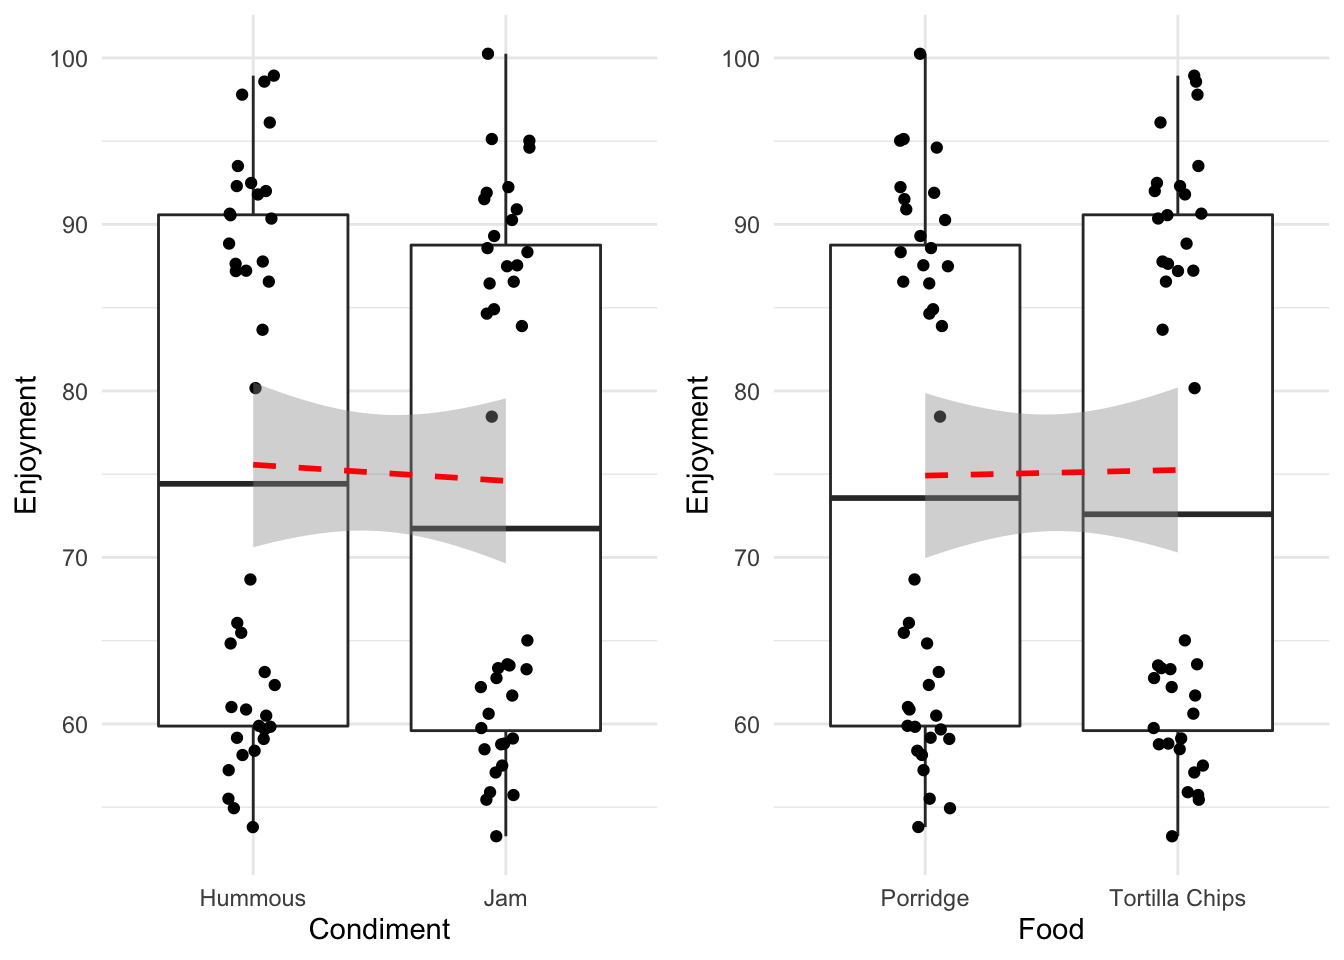
\includegraphics{intro_to_stats_files/figure-latex/unnamed-chunk-79-1.pdf}

in the way that the output we've seen so far has it, this would be

\begin{quote}
Porridge - Tortilla Chips == 0

Hummous - Jam == 0
\end{quote}

Let's also see whether \texttt{food\ *\ condiment} has an effect. This would be like the interaction situation.

\begin{quote}
Porridge:Jam - Tortilla Chips:Jam == 0

Porridge:Hummous - Tortilla Chips:Hummous == 0
\end{quote}

\begin{Shaded}
\begin{Highlighting}[]
\KeywordTok{its_food_two_ways_time}\NormalTok{()}
\end{Highlighting}
\end{Shaded}

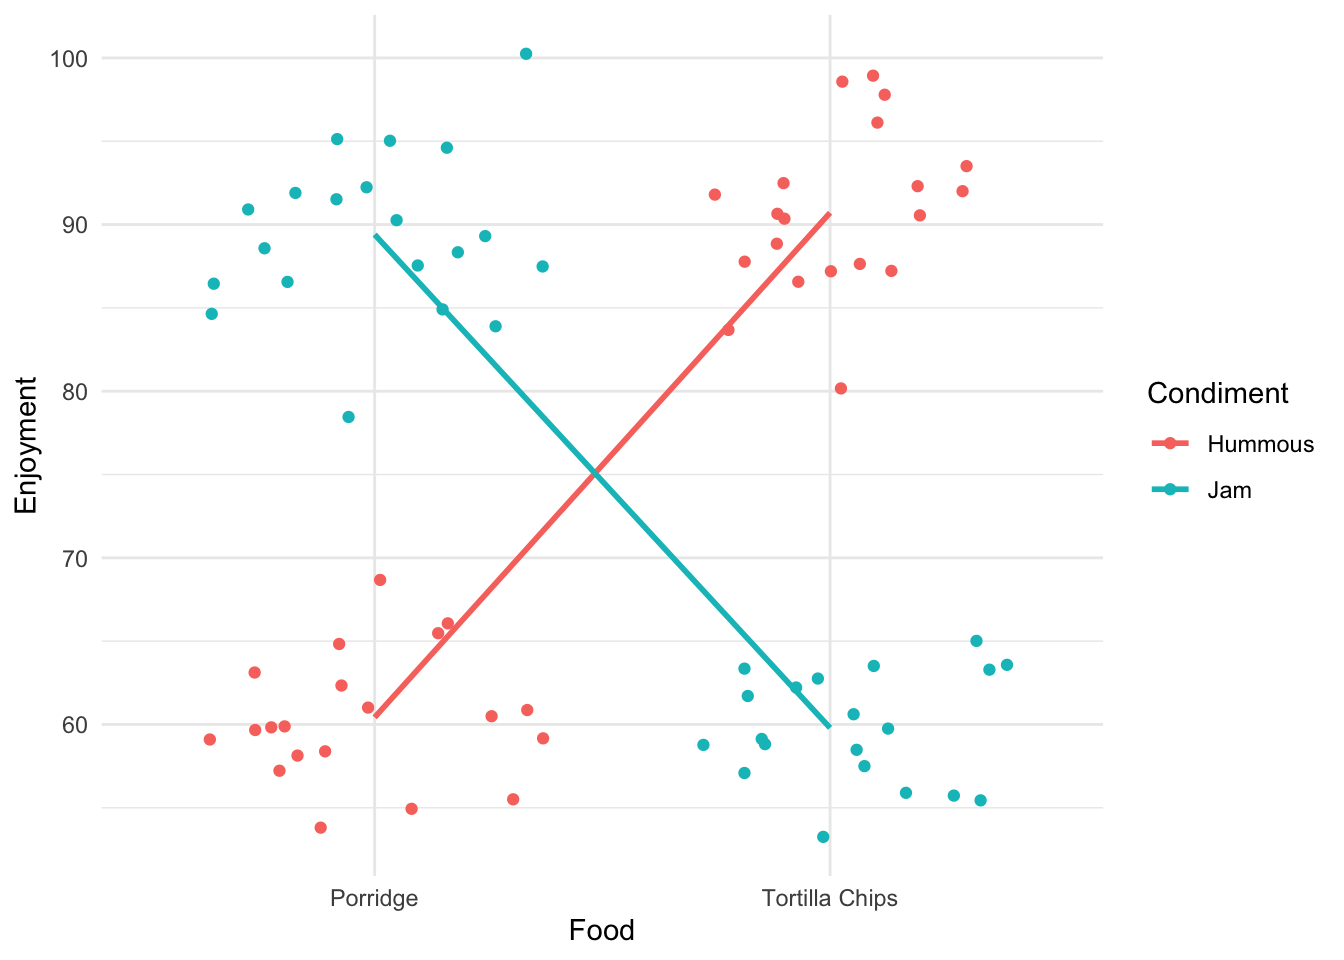
\includegraphics{intro_to_stats_files/figure-latex/unnamed-chunk-80-1.pdf}

So we have four lines of interest to look at - four contrasts.

For the two main non-interaction effects we could think to look at these as we've done before, using the \texttt{mcp()} function with the \texttt{interaction\_model} with the explicit interaction in it, like this

\begin{Shaded}
\begin{Highlighting}[]
\KeywordTok{summary}\NormalTok{(}
  \KeywordTok{glht}\NormalTok{(interaction_model, }\DataTypeTok{linfct =} \KeywordTok{mcp}\NormalTok{(}
    \DataTypeTok{Food =} \StringTok{"Tukey"}\NormalTok{,}
    \DataTypeTok{Condiment =} \StringTok{"Tukey"}
\NormalTok{  ))}
\NormalTok{)}
\end{Highlighting}
\end{Shaded}

\begin{verbatim}
## Warning in mcp2matrix(model, linfct = linfct): covariate interactions found --
## default contrast might be inappropriate

## Warning in mcp2matrix(model, linfct = linfct): covariate interactions found --
## default contrast might be inappropriate
\end{verbatim}

\begin{verbatim}
## 
## 	 Simultaneous Tests for General Linear Hypotheses
## 
## Multiple Comparisons of Means: Tukey Contrasts
## 
## 
## Fit: lm(formula = Enjoyment ~ Food + Condiment + Food:Condiment, data = food)
## 
## Linear Hypotheses:
##                                      Estimate Std. Error t value Pr(>|t|)    
## Food: Tortilla Chips - Porridge == 0   30.282      1.351   22.41   <1e-10 ***
## Condiment: Jam - Hummous == 0          28.974      1.351   21.45   <1e-10 ***
## ---
## Signif. codes:  0 '***' 0.001 '**' 0.01 '*' 0.05 '.' 0.1 ' ' 1
## (Adjusted p values reported -- single-step method)
\end{verbatim}

This gives a result, but actually throws up a warning. Since we have an interaction term in our model, we have a complication. The \texttt{glht()} function has spotted that there are interacting terms and potential for confounding and the \(p\)-values are therefore a bit suspect without being a bit more careful. We need to take account of the interaction as a term of its own in our hypothesis tests. Annoyingly, this isn't an easy thing to specify in the \texttt{glht()} function and the easiest way in practice is to just do all the comparisons.

\begin{sidenote}
The reason that the warnings are thrown in the interaction model is to do with an ANOVA internal object called the Contrasts Matrix, which specifies the contrasts and is used in the linear algebra of the ANOVA and Tukey's method. The Contrast Matrix is basically a grid with the different samples and contrasts as the rows and columns with a load of ones and zeroes in it. For Tukey's method to work the Contrast Matrix should be `orthogonal', which roughly means symmetric around a certain axis. When we get the interaction term in the model we lose the orthogonality in the Contrast Matrix and Tukey's method stops working well. The orthogonality is one of the assumptions that statisticians talk about. It is possible to set up different Contrast Matrices and there are methods for getting significance for non-orthogonal ones, however that does take us a bit too far into theory. For most purposes, except for those with very large numbers of variables it is convenient to use the alternative method below.
\end{sidenote}

\hypertarget{doing-all-pairwise-interactions}{%
\section{Doing all pairwise interactions}\label{doing-all-pairwise-interactions}}

Although we're interested in only two specific interactions, usually it's easier to do all pairwise comparisons in one step, as we don't often have so many interacting variables that it gets unwieldy. To do this we must add an interaction column to our data and model that. The \texttt{interaction()} function is built for just this reason and allows us to add an interaction column directly from existing data.

\begin{Shaded}
\begin{Highlighting}[]
\NormalTok{food_}\DecValTok{2}\NormalTok{ <-}\StringTok{ }\NormalTok{food }\OperatorTok\StringTok{ }\NormalTok{dplyr}\OperatorTok{::}\KeywordTok{mutate}\NormalTok{(}\DataTypeTok{FoodCondiment =} \KeywordTok{interaction}\NormalTok{(Food, Condiment))}
\NormalTok{knitr}\OperatorTok{::}\KeywordTok{kable}\NormalTok{( food_}\DecValTok{2}\NormalTok{[}\KeywordTok{c}\NormalTok{(}\DecValTok{1}\NormalTok{,}\DecValTok{21}\NormalTok{,}\DecValTok{41}\NormalTok{,}\DecValTok{61}\NormalTok{),] , }\DataTypeTok{align =} \StringTok{"c"}\NormalTok{)}
\end{Highlighting}
\end{Shaded}

\begin{tabular}{l|c|c|c|c}
\hline
  & Food & Condiment & Enjoyment & FoodCondiment\\
\hline
1 & Tortilla Chips & Hummous & 87.19762 & Tortilla Chips.Hummous\\
\hline
21 & Tortilla Chips & Jam & 55.72871 & Tortilla Chips.Jam\\
\hline
41 & Porridge & Hummous & 57.22117 & Porridge.Hummous\\
\hline
61 & Porridge & Jam & 91.89820 & Porridge.Jam\\
\hline
\end{tabular}

We can see that all we've done is add a column that describes the interaction. We can use this in the place of the individual variables as before and now don't need to explicitly mention the interaction in the specification because it is modelled implicitly in the new column. That means our model looks like this

\begin{Shaded}
\begin{Highlighting}[]
\NormalTok{interaction_model2 <-}\StringTok{ }\KeywordTok{lm}\NormalTok{(Enjoyment }\OperatorTok{~}\StringTok{ }\NormalTok{FoodCondiment, }\DataTypeTok{data =}\NormalTok{ food_}\DecValTok{2}\NormalTok{)}
\end{Highlighting}
\end{Shaded}

To do the contrasts we can use the single interaction column as the target of Tukey.

\begin{Shaded}
\begin{Highlighting}[]
\KeywordTok{summary}\NormalTok{(}
  \KeywordTok{glht}\NormalTok{(interaction_model2, }\DataTypeTok{linfct =} \KeywordTok{mcp}\NormalTok{(}\DataTypeTok{FoodCondiment =} \StringTok{"Tukey"}\NormalTok{))}
\NormalTok{  )}
\end{Highlighting}
\end{Shaded}

\begin{verbatim}
## 
## 	 Simultaneous Tests for General Linear Hypotheses
## 
## Multiple Comparisons of Means: Tukey Contrasts
## 
## 
## Fit: lm(formula = Enjoyment ~ FoodCondiment, data = food_2)
## 
## Linear Hypotheses:
##                                                  Estimate Std. Error t value
## Tortilla Chips.Hummous - Porridge.Hummous == 0     30.282      1.351  22.414
## Porridge.Jam - Porridge.Hummous == 0               28.974      1.351  21.446
## Tortilla Chips.Jam - Porridge.Hummous == 0         -0.631      1.351  -0.467
## Porridge.Jam - Tortilla Chips.Hummous == 0         -1.308      1.351  -0.968
## Tortilla Chips.Jam - Tortilla Chips.Hummous == 0  -30.913      1.351 -22.881
## Tortilla Chips.Jam - Porridge.Jam == 0            -29.605      1.351 -21.913
##                                                  Pr(>|t|)    
## Tortilla Chips.Hummous - Porridge.Hummous == 0     <1e-05 ***
## Porridge.Jam - Porridge.Hummous == 0               <1e-05 ***
## Tortilla Chips.Jam - Porridge.Hummous == 0          0.966    
## Porridge.Jam - Tortilla Chips.Hummous == 0          0.768    
## Tortilla Chips.Jam - Tortilla Chips.Hummous == 0   <1e-05 ***
## Tortilla Chips.Jam - Porridge.Jam == 0             <1e-05 ***
## ---
## Signif. codes:  0 '***' 0.001 '**' 0.01 '*' 0.05 '.' 0.1 ' ' 1
## (Adjusted p values reported -- single-step method)
\end{verbatim}

We can see all possible interaction groupings and lines, without any warnings. We can see that the significances make good sense. The Porridge and Jam is no more enjoyable than the Tortilla Chips and Hummous, the Porridge and Hummous is no more enjoyable than the Tortilla Chips and Jam and all the other match and mismatch food and condiments are as we might expect from this very obviously loaded example.

We said we wanted to look specifically at the interaction between the Porridge with Jam and Tortilla Chips with Jam - we can see that there is a significant difference in enjoyment, about 29 points. Similarly Porridge with Hummous is less enjoyable than Tortilla Chips with Hummous, by about 30 points.

\hypertarget{summary}{%
\section{Summary}\label{summary}}

We've looked at how to use linear models to think about differences between lots of categories and at what it means for variables to be interacting. We learned that ANOVA is inherently a test based on a linear model that is designed to do all comparisons at once and we learned how to carry the ANOVAs out having built the proper linear model for cases with and without interactions. We know all we need to use R to perform ANOVAs with linear models - which always use linear models anyway.

\hypertarget{extra-credit-anova-model-level-p-and-as-a-hypothesis-test}{%
\section{\texorpdfstring{Extra Credit: ANOVA model-level \(p\) and as a hypothesis test}{Extra Credit: ANOVA model-level p and as a hypothesis test}}\label{extra-credit-anova-model-level-p-and-as-a-hypothesis-test}}

Recall that when we introduced linear models we looked at the statistics of the coefficients (the column \(Pr(>|t|)\) in the coefficient block of the summary) \emph{and} the statistics of the whole model, the \(p\)-value at the end.

When we did the simple linear model as an alternative of the \(t\)-test, then these two \(p\)-values were the same - this is because the model then only had one coefficient, so the \(p\) of that coefficient was the overall \(p\). With more than one coefficient, then the overall model score is made up differently. The overall model can be significant, whereas the individual variables/groups/coefficient within may not be. That's what we saw when we looked at the \texttt{PlantGrowth} data.

\begin{Shaded}
\begin{Highlighting}[]
\KeywordTok{summary}\NormalTok{(model)}
\end{Highlighting}
\end{Shaded}

\begin{verbatim}
## 
## Call:
## lm(formula = weight ~ group, data = PlantGrowth)
## 
## Residuals:
##     Min      1Q  Median      3Q     Max 
## -1.0710 -0.4180 -0.0060  0.2627  1.3690 
## 
## Coefficients:
##             Estimate Std. Error t value Pr(>|t|)    
## (Intercept)   5.0320     0.1971  25.527   <2e-16 ***
## grouptrt1    -0.3710     0.2788  -1.331   0.1944    
## grouptrt2     0.4940     0.2788   1.772   0.0877 .  
## ---
## Signif. codes:  0 '***' 0.001 '**' 0.01 '*' 0.05 '.' 0.1 ' ' 1
## 
## Residual standard error: 0.6234 on 27 degrees of freedom
## Multiple R-squared:  0.2641,	Adjusted R-squared:  0.2096 
## F-statistic: 4.846 on 2 and 27 DF,  p-value: 0.01591
\end{verbatim}

None of the reported variable/group/coefficient values are significant but the model level \(p\) is. This indicates that one of the groups is significant. This is because the ANOVA as a test tests the hypothesis that all lines between groups have slopes of zero. When one line isn't likely to have a zero slope the model \(p\) is low

In terms of a formal hypothesis test what we're asking amounts to an extension to what we saw with the \(t\)-test:

\begin{itemize}
\tightlist
\item
  All flat lines with slopes of zero is equivalent to the Null hypothesis

  \begin{itemize}
  \tightlist
  \item
    \(H_{0}\) the group means are \emph{all} equal
  \end{itemize}
\item
  At least one \(p\)-value that suggests the slope is rare is equivalent to the Alternative hypothesis

  \begin{itemize}
  \tightlist
  \item
    \(H_{1}\) the group means are not \emph{all} equal
  \end{itemize}
\end{itemize}

In other words we can think of the ANOVA testing the idea that all the groups are the result of random sampling from all the observations, if this were true the slopes between groups would all be the same.

It's by using the \emph{post-hoc} tests like Tukey's we get at the specific differences between groups.

\hypertarget{extra-credit-testing-specific-interactions}{%
\section{Extra Credit: Testing specific interactions}\label{extra-credit-testing-specific-interactions}}

The table output is a bit rich and confusing, you can get a simpler output at the expense of some more work. For the two sets of interactions we're interested in we can look at them specifically but naming them explicitly in \texttt{glht} is trickier than we've done so far.

We have to specify a matrix of comparisons ourselves. The first step is to work out all the different interactions of the levels of the \texttt{food*condiment} interaction term. We can do that with the \texttt{interaction()} function

\begin{Shaded}
\begin{Highlighting}[]
\NormalTok{f_c_interactions <-}\StringTok{ }\KeywordTok{interaction}\NormalTok{(food}\OperatorTok{$}\NormalTok{Food, food}\OperatorTok{$}\NormalTok{Condiment, }\DataTypeTok{sep=}\StringTok{":"}\NormalTok{)}
\KeywordTok{head}\NormalTok{(f_c_interactions)}
\end{Highlighting}
\end{Shaded}

\begin{verbatim}
## [1] Tortilla Chips:Hummous Tortilla Chips:Hummous Tortilla Chips:Hummous
## [4] Tortilla Chips:Hummous Tortilla Chips:Hummous Tortilla Chips:Hummous
## 4 Levels: Porridge:Hummous Tortilla Chips:Hummous ... Tortilla Chips:Jam
\end{verbatim}

We can see that this is just a factor object with all the combinations of \texttt{Food} and \texttt{Condiment}. Using the \texttt{levels()} function gives us all the unique values in the order that R will use them.

\begin{Shaded}
\begin{Highlighting}[]
\KeywordTok{levels}\NormalTok{(f_c_interactions)}
\end{Highlighting}
\end{Shaded}

\begin{verbatim}
## [1] "Porridge:Hummous"       "Tortilla Chips:Hummous" "Porridge:Jam"          
## [4] "Tortilla Chips:Jam"
\end{verbatim}

Now we can make the matrix, our eventual matrix will look like this

\begin{verbatim}
##                                           Porridge:Hummous
## Porridge:Jam - Tortilla Chips:Jam                        0
## Porridge:Hummous - Tortilla Chips:Hummous                1
##                                           Tortilla Chips:Hummous Porridge:Jam
## Porridge:Jam - Tortilla Chips:Jam                              0            1
## Porridge:Hummous - Tortilla Chips:Hummous                     -1            0
##                                           Tortilla Chips:Jam
## Porridge:Jam - Tortilla Chips:Jam                         -1
## Porridge:Hummous - Tortilla Chips:Hummous                  0
\end{verbatim}

We can see that there is a row per comparison and a column per possible interaction. At the intersection we write a zero if we don't want to include that possible interaction in the contrast, a 1 if we want it to be the first part and a -1 if we want it to be the second part (IE, the part after the minus sign).

As the \texttt{levels()} function gives us the order, we set up the rows one by one and join them together.

\begin{Shaded}
\begin{Highlighting}[]
\NormalTok{P.J_TC.J <-}\StringTok{ }\KeywordTok{c}\NormalTok{(}\DecValTok{0}\NormalTok{,}\DecValTok{0}\NormalTok{,}\DecValTok{1}\NormalTok{,}\OperatorTok{-}\DecValTok{1}\NormalTok{)}
\NormalTok{P.H_TC.H <-}\StringTok{ }\KeywordTok{c}\NormalTok{(}\DecValTok{1}\NormalTok{,}\OperatorTok{-}\DecValTok{1}\NormalTok{,}\DecValTok{0}\NormalTok{,}\DecValTok{0}\NormalTok{)}
\end{Highlighting}
\end{Shaded}

Now we can stick them together, use the \texttt{levels()} function as the column names and add row names. Note you can call the rows what you like, so you dont have to use the long names, but the columns \emph{must} be named and ordered according to the \texttt{levels()} function

\begin{Shaded}
\begin{Highlighting}[]
\NormalTok{contr_of_interest <-}\StringTok{ }\KeywordTok{rbind}\NormalTok{(P.J_TC.J, P.H_TC.H)}
\KeywordTok{colnames}\NormalTok{(contr_of_interest) <-}\StringTok{ }\KeywordTok{levels}\NormalTok{(f_c_interactions)}
\KeywordTok{rownames}\NormalTok{(contr_of_interest) <-}\StringTok{ }\KeywordTok{c}\NormalTok{(}\StringTok{"P:J - TC:J"}\NormalTok{,}
          \StringTok{"P:H - TC:H"}\NormalTok{)}

\NormalTok{contr_of_interest}
\end{Highlighting}
\end{Shaded}

\begin{verbatim}
##            Porridge:Hummous Tortilla Chips:Hummous Porridge:Jam
## P:J - TC:J                0                      0            1
## P:H - TC:H                1                     -1            0
##            Tortilla Chips:Jam
## P:J - TC:J                 -1
## P:H - TC:H                  0
\end{verbatim}

Now we can do the test using the custom matrix.

\begin{Shaded}
\begin{Highlighting}[]
\KeywordTok{summary}\NormalTok{(}\KeywordTok{glht}\NormalTok{( interaction_model, }\DataTypeTok{linfct =}\NormalTok{ contr_of_interest))}
\end{Highlighting}
\end{Shaded}

\begin{verbatim}
## 
## 	 Simultaneous Tests for General Linear Hypotheses
## 
## Fit: lm(formula = Enjoyment ~ Food + Condiment + Food:Condiment, data = food)
## 
## Linear Hypotheses:
##                 Estimate Std. Error t value Pr(>|t|)    
## P:J - TC:J == 0   88.862      3.021   29.41   <1e-10 ***
## P:H - TC:H == 0   30.144      2.136   14.11   <1e-10 ***
## ---
## Signif. codes:  0 '***' 0.001 '**' 0.01 '*' 0.05 '.' 0.1 ' ' 1
## (Adjusted p values reported -- single-step method)
\end{verbatim}

And there we have the specific interaction contrasts. Note how in doing this we don't generate any warnings even though we used the model with the explicit interaction term, this is because when we generate our own contrast matrix like this we get an appropriate orthogonality for the test.

\begin{roundup}
\begin{itemize}
\tightlist
\item
  Working with multiple variables goes the same as working with just one
\item
  ANOVA is a flexible tool for specifying comparisons between variables in linear models
\end{itemize}
\end{roundup}

\begin{task}
\end{task}

\hypertarget{non-parametric-tests-and-linear-models}{%
\chapter{Non-parametric tests and linear models}\label{non-parametric-tests-and-linear-models}}

\begin{enumerate}
\def\labelenumi{\arabic{enumi}.}
\tightlist
\item
  Questions
\end{enumerate}

\begin{itemize}
\tightlist
\item
  How do I can I analyse data in non-numeric scales?
\item
  What are the common mistakes when analysing non-numeric data?
\end{itemize}

\begin{enumerate}
\def\labelenumi{\arabic{enumi}.}
\setcounter{enumi}{1}
\tightlist
\item
  Objectives
\end{enumerate}

\begin{itemize}
\tightlist
\item
  Learn how to spot the places we mix up categoric and non-categoric data
\item
  Understand how to use ranked data in a linear model
\item
  Understand ordered and unordered factors
\end{itemize}

\begin{enumerate}
\def\labelenumi{\arabic{enumi}.}
\setcounter{enumi}{2}
\tightlist
\item
  Keypoints
\end{enumerate}

\begin{itemize}
\tightlist
\item
  Using numbers as names does not make data quantitative
\item
  Ranking data makes it possible to analyse ordered categoric data in a linear model
\end{itemize}

So far we've looked at tests where the dependent or response measurement has been continuous, that is a measurable number on a continuous scale, like mass or fluorescence. In this section we'll look at how straight lines can be used to understand differences when we have a discrete or categorical response output. A discrete response variable is one where we have certain categories of result, `tall' or `short', `dead' or `alive' or `infected' or `not'. You'll likely be familiar with these approaches from such things as the chi-squared (\(\chi^2\)) test or other so-called `non-parametric' test like the Mann-Whitney.

We'll start by looking at how these data really are different from the data we've used already, common mistakes are always enlightening.

\hypertarget{common-misrepresentations-of-discrete-data}{%
\section{Common misrepresentations of discrete data}\label{common-misrepresentations-of-discrete-data}}

A common place where analysing discrete data goes wrong is when the analyst confuses the categoric with the continuous, this is often caused by a bad naming scheme as much as a lack of appreciation of the real nature of the data. Often, using numbers as the names for categories can lead the unaware analyst to make a critical mistake. Let's consider a plant infection assay (sometimes called an HR assay). Here a large-ish leaf of a plant is infected at points on its surface with either different strains or varieties of some pathogen and controls. After a period of incubation the severity of disease at each patch is assessed by eye and a score of disease applied. Sometimes that score will be a numeric one that may be like this example from Supplemental Figure 1 A in a 2020 PNAS paper by Gao et al.~\citet{Gao9613}

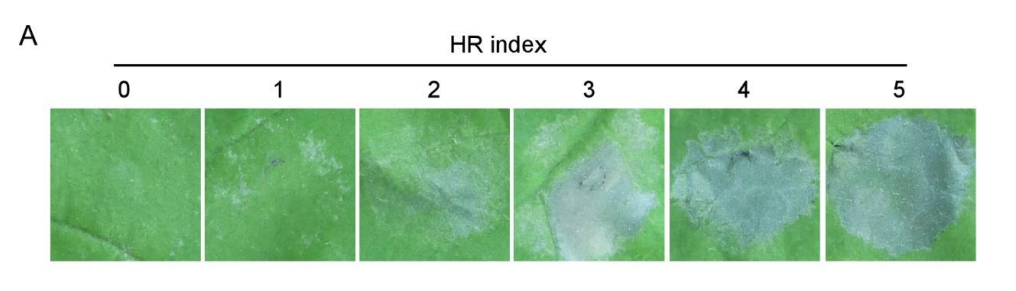
\includegraphics{fig/dong_figs1A.png}
In the figure we can see that a number has been attached to a category, roughly an amount of disease. The numbers increase as disease does but it is a very rough and therefore discontinuous fit. The change in size in numbers don't relate to each other in the same way that the changes in disease do. The unit difference from 0 to 1 doesn't seem to be copied in any of the other units and 5 doesnt have just 5 times more apparent disease than 1. The scale has numbers in it, but it isn't continuous.

We can see what the scale represents if we try and use words to express the categories.

\begin{Shaded}
\begin{Highlighting}[]
\KeywordTok{library}\NormalTok{(itssl)}
\KeywordTok{its_hr_score_scheme_time}\NormalTok{()}
\end{Highlighting}
\end{Shaded}

\begin{tabular}{c|c}
\hline
severity & score\\
\hline
Dead & 4\\
\hline
Very Ill & 3\\
\hline
Ill & 2\\
\hline
No Effect & 1\\
\hline
\end{tabular}

Which looks fine at first glance, but again isn't continuous.

Typically this will be used in a replicated infection experiment and give data that look like this when collected, which is where the problem arises.

\begin{Shaded}
\begin{Highlighting}[]
\NormalTok{scores <-}\StringTok{ }\KeywordTok{its_hr_scores_time}\NormalTok{()}
\NormalTok{scores }\OperatorTok\StringTok{ }\KeywordTok{its_table_time}\NormalTok{()}
\end{Highlighting}
\end{Shaded}

\begin{tabular}{c|c|c}
\hline
strain & replicate & score\\
\hline
control & 1 & 1\\
\hline
mild & 1 & 3\\
\hline
deadly & 1 & 4\\
\hline
control & 2 & 2\\
\hline
mild & 2 & 3\\
\hline
deadly & 2 & 4\\
\hline
control & 3 & 1\\
\hline
mild & 3 & 3\\
\hline
deadly & 3 & 3\\
\hline
\end{tabular}

We now have a table that looks to computers and humans alike as if it is full of numbers, which it isn't, its full of numbers in the place of words. A simple mental test is to try and use the categories as numbers and see if they behave. For example, is a score of `2' twice that of `1', in this case, is `Ill' twice the effect of `No Effect'? Clearly it isn't, confirming that these numbers aren't continuous numbers at all, merely place holders for some other conception of the severity of the disease.

The problem is exacerbated by not paying attention to this and jumping straight to a plot. Consider this:

\begin{Shaded}
\begin{Highlighting}[]
\KeywordTok{library}\NormalTok{(ggplot2)}
\NormalTok{scores }\OperatorTok\StringTok{ }\KeywordTok{ggplot}\NormalTok{() }\OperatorTok{+}\StringTok{ }
\StringTok{  }\KeywordTok{aes}\NormalTok{(strain, score) }\OperatorTok{+}\StringTok{ }
\StringTok{  }\KeywordTok{geom_jitter}\NormalTok{(}\KeywordTok{aes}\NormalTok{(}\DataTypeTok{colour =}\NormalTok{ replicate))}
\end{Highlighting}
\end{Shaded}

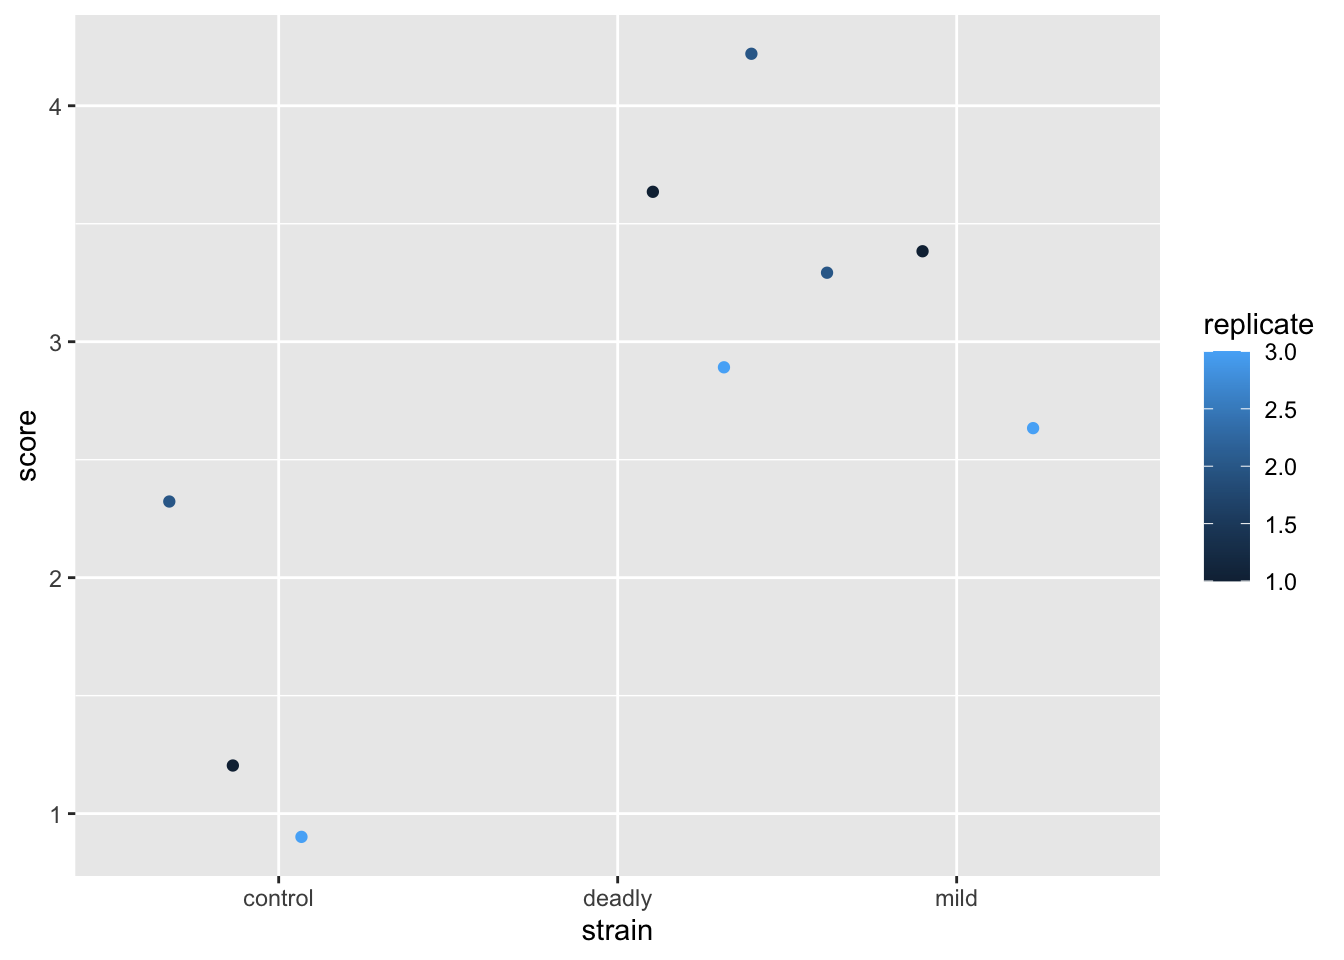
\includegraphics{intro_to_stats_files/figure-latex/unnamed-chunk-97-1.pdf}

Looks good?

No.~By the sweet warmth of the first suns of spring, no.

These data are misrepresented by this plot. There are some alarm bells that should ring when we look at this. The first is that scale for replicate. The scale shows replicate values like 1.5 and 2.5 - we didn't do a replicate 1.5 (not least because it doesn't make sense to do a replicate .5). So why has \texttt{ggplot} drawn that scale - because it saw numbers and assumed the data in this column are continuous and not discrete. This needs fixing, the replicate is a category, really, not a number. We wouldn't lose any meaning if we used \texttt{A,B,C} or \texttt{one,two,three} and while the computer is good at recognising text as categories, it just thinks the numbers are real numbers. So we'll need to avoid doing this, or be prepared to correct it.

\begin{sidenote}
By using numbers for our score, then we have been able to use `geom\_jitter()' as a representation and it has generated additions to the scores that leave it with decimal points and that isn't correct either. It seems defensible on the grounds that if we didn't use geom\_jitter() all the points would be in one place but to avoid the problem we should be doing something very different in the first place.
\end{sidenote}

\hypertarget{twisting-names-into-numbers-confuses-the-mind}{%
\subsection{Twisting names into numbers confuses the mind}\label{twisting-names-into-numbers-confuses-the-mind}}

The next level of mistake that follows from believing that the scores are numbers is treating them like numbers. We often see the plot evolve in this manner

\begin{Shaded}
\begin{Highlighting}[]
\NormalTok{scores }\OperatorTok\StringTok{ }\KeywordTok{ggplot}\NormalTok{() }\OperatorTok{+}\StringTok{ }
\StringTok{  }\KeywordTok{aes}\NormalTok{(strain, score) }\OperatorTok{+}\StringTok{ }
\StringTok{  }\KeywordTok{geom_boxplot}\NormalTok{() }\OperatorTok{+}\StringTok{ }
\StringTok{  }\KeywordTok{geom_jitter}\NormalTok{(}\KeywordTok{aes}\NormalTok{(}\DataTypeTok{colour =}\NormalTok{ replicate))}
\end{Highlighting}
\end{Shaded}

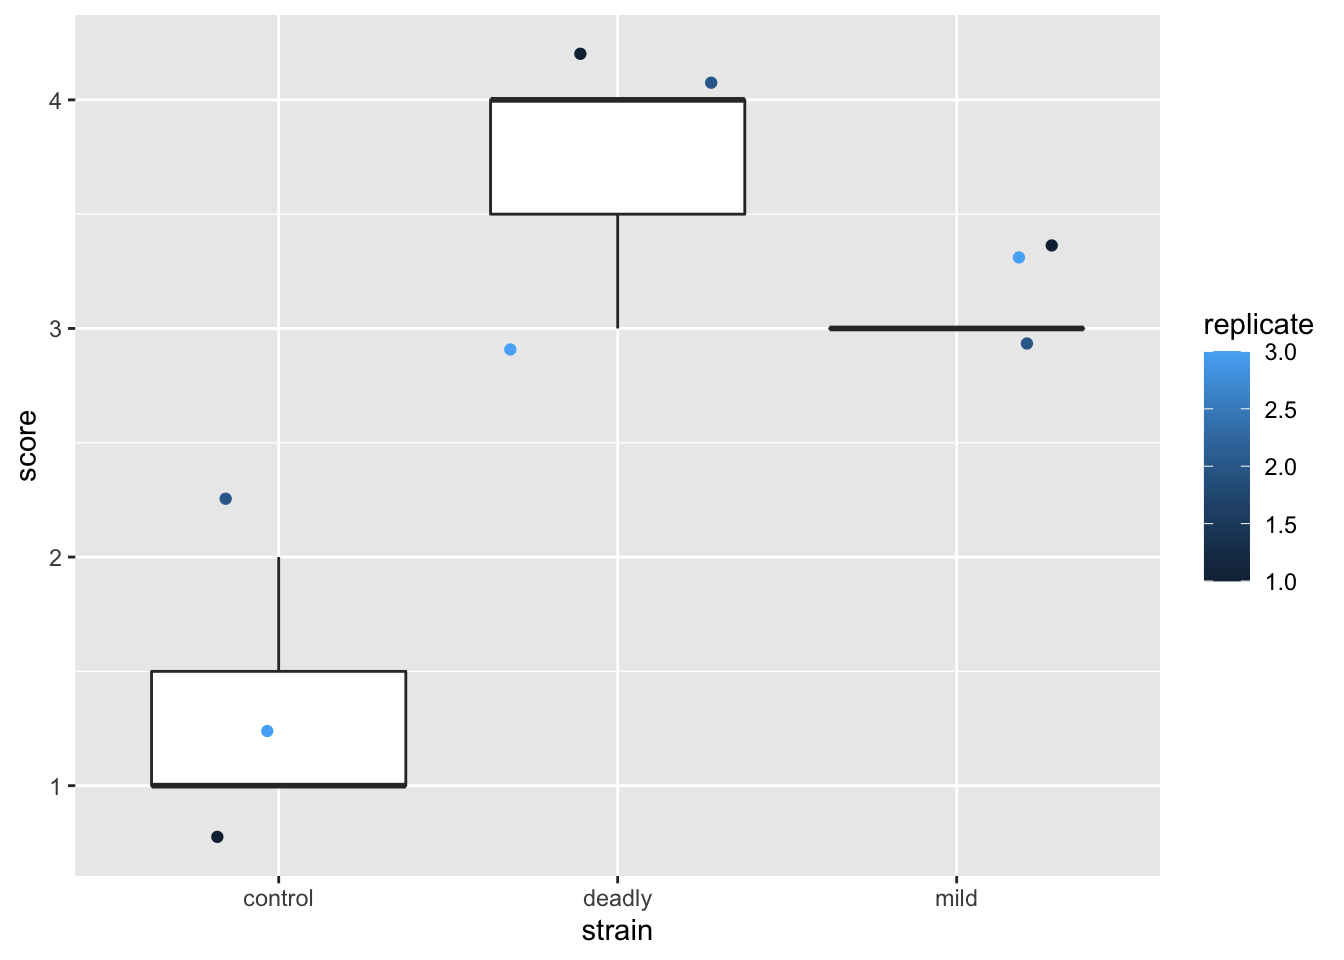
\includegraphics{intro_to_stats_files/figure-latex/unnamed-chunk-99-1.pdf}

What the cuss? This is a dreadful misrepresentation of the data!

This plot makes us see things that aren't really there - particularly statistics like means and ranges, and relative magnitude differences between categories.

\hypertarget{this-does-not-mean-what-i-think-you-think-it-means}{%
\subsection{This does not mean what I think you think it means}\label{this-does-not-mean-what-i-think-you-think-it-means}}

Well, not you specifically, but someone. Someone definitely thinks what I think they think it means because this mistake keeps coming up.\\
We think we can see these statistics because the boxplot shows them. But the boxplot is a dreamlike fabrication. The things it purports to show like the mean of the data, its interquartile range etc are each a numeric feature calculated using formulae based on numbers. But these data are not numbers - they are category names that happen to have digits to represent them. We've squeezed numbers in where no numbers should be and invented statistical lies.

The use of numbers as names for the categories created a problem of mental overloading - simultaneaously knowing that the data are categorical and treating them as continuous. Believing that because we've used numbers for categories we can treat them as numbers. On top of this the presentation tricks our mind into considering the results as if these statistics were real.

If we use the actual category names we see how ridiculous the boxplot is - consider \texttt{mean(Ill,\ No\ Effect,\ Ill)\ =\ 0.66}, it doesn't make any sense. By using numbers as proxies for our categories, we've confused the issue and the knock-on effect is that we start to read (conciously or unconciously) things we shouldn't from the plot. One unavoidable impression from the plot is that `mild' strain is somehow about 3/4 of the badness of the `deadly' strain. Does that mean the plants were three-quarters dead? Of course not. The misrepresentation in these plots leaves with bad intuition about the relationships in our data.

The use of boxplots to show categories is seductive, it gives an impression of transparency and apparent differences when we use numbers, this is a case where the road to hell is paved with good intentions.

With these plots as a base the analysts next move is to run statistical analysis in the way we have learned and, sadly, generate results that are worse than meaningless.

And indeed this does happen in published results, see this figure from the same Gao et al \citet{Gao9613} paper .

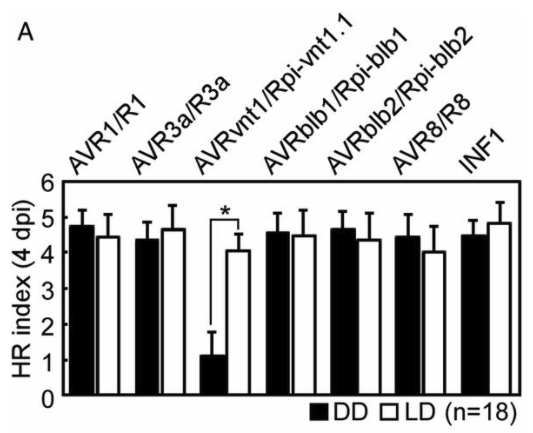
\includegraphics{fig/dong_fig1A.png}
A barchart with all the errors we mentioned, the bars represent means, the error bars represent standard errors and the legend reports an ANOVA done on these data that concludes a significant reduction in the one low sample.

\hypertarget{build-a-strong-foundation}{%
\subsection{Build a strong foundation}\label{build-a-strong-foundation}}

We must avoid these category confusions. There are some key places we can do this in our analysis workflow

\begin{itemize}
\tightlist
\item
  Know and declare the proper data type to R
\item
  Use a statistical test/model type appropriate to the datatype
\end{itemize}

When we load our data into R, we'll need to make sure that we use the right data types. As a result of this we'll find that the plots we try to make will come out more appropriately - R will adapt to the data as far as it can. Second, when it comes to doing hypothesis tests we will have to use the proper test for the data type. As we are using the linear model as the basis for our interpretations we'll need to learn the adaptations to that.

In the rest of this chapter we'll look at correctly describing data to R, creating an appropriate plot for some data and then back to our main thread - using the linear model as a basis for our understanding of statistical tests - this time with categorical response variable.

\hypertarget{setting-type-properly}{%
\section{Setting type properly}\label{setting-type-properly}}

At the start of an analysis, when we're loading data into R is our best opportunity to correct datatype, before we've done any work on it and before it starts to get in the way. In a lot of everyday cases we'll be loading text in from an Excel file or something similar like a \texttt{.csv} or \texttt{.txt} file, so that will be our example case.

\begin{sidenote}
Base R provides the `read.csv()' (\emph{read dot csv}) function for us to load `.csv' files and no option for loading Excel files. The tidyverse packages readr and readxl provide the read\_csv() and read\_excel() (\emph{read underscore csv}) options respectively. You'll see read.csv() a lot in older code and quick tutorials, but it is a bit clunky. Some of read.csv()'s default behaviours can be a bit unpredictable and we have to undo some of its work sometimes. So we'll look at the more consistent tidyverse offerings.
\end{sidenote}

\hypertarget{setting-type-with-read_csv}{%
\subsection{\texorpdfstring{Setting type with \texttt{read\_csv()}}{Setting type with read\_csv()}}\label{setting-type-with-read_csv}}

On loading data with \texttt{read\_csv()}, we get a column specification - this tells us what R thinks each column contained, we must check it carefully to make sure R understands the data as you do. Here we'll load in the mock HR data we used above.

\begin{Shaded}
\begin{Highlighting}[]
\KeywordTok{library}\NormalTok{(readr)}
\KeywordTok{read_csv}\NormalTok{(}\StringTok{"data/sample.csv"}\NormalTok{)}
\end{Highlighting}
\end{Shaded}

\begin{verbatim}
## 
## -- Column specification --------------------------------------------------------
## cols(
##   strain = col_character(),
##   replicate = col_double(),
##   score = col_double()
## )
\end{verbatim}

\begin{verbatim}
## # A tibble: 9 x 3
##   strain  replicate score
##   <chr>       <dbl> <dbl>
## 1 control         1     1
## 2 mild            1     3
## 3 deadly          1     4
## 4 control         2     2
## 5 mild            2     3
## 6 deadly          2     4
## 7 control         3     1
## 8 mild            3     3
## 9 deadly          3     3
\end{verbatim}

So we can see that R thinks the column \texttt{strain} contains \texttt{character} data (text), and the \texttt{replicate} and \texttt{strain} column data are \texttt{double} (numeric type) data. Well, almost one out of three is pretty bad. Although we (foolishly) coded the categoric \texttt{replicate} and \texttt{strain} as numbers, they aren't, they're categories (or factors, in statistic parlance). We can use a column specification in the \texttt{read\_csv()} function to force these to be factors.

\begin{sidenote}
Factors are a statistical name for a categorical variable. Each factor is made up of one or more `levels' the different values that factor can take. In our HR score data, the factor would be `score' and it's levels would be `3',`1',`2' and `4'. There are lots of tools that work with factors in R, they are a common object.
\end{sidenote}

The \texttt{col\_factor()} function tells R that these columns should be a factor when loading.

\begin{Shaded}
\begin{Highlighting}[]
\KeywordTok{read_csv}\NormalTok{(}
  \StringTok{"data/sample.csv"}\NormalTok{,}
  \DataTypeTok{col_types =} \KeywordTok{cols}\NormalTok{(}
    \DataTypeTok{strain =} \KeywordTok{col_factor}\NormalTok{(}\OtherTok{NULL}\NormalTok{),}
    \DataTypeTok{replicate =} \KeywordTok{col_factor}\NormalTok{(}\OtherTok{NULL}\NormalTok{),}
    \DataTypeTok{score =} \KeywordTok{col_factor}\NormalTok{(}\OtherTok{NULL}\NormalTok{)}
\NormalTok{  )}
\NormalTok{)}
\end{Highlighting}
\end{Shaded}

\begin{verbatim}
## # A tibble: 9 x 3
##   strain  replicate score
##   <fct>   <fct>     <fct>
## 1 control 1         1    
## 2 mild    1         3    
## 3 deadly  1         4    
## 4 control 2         2    
## 5 mild    2         3    
## 6 deadly  2         4    
## 7 control 3         1    
## 8 mild    3         3    
## 9 deadly  3         3
\end{verbatim}

This is much better, R now knows not to treat any of those columns as numbers, so the mistakes we're trying to avoid are much less likely to happen.

We can go one step further and explicitly state the allowed values in a factor. When we do this we get to pick the order that R will deal with them in (and this is important in our data because control \textless{} mild \textless{} deadly in some sense) and it will spot when we try to load in a factor level that we haven't declared, which can save us headaches down the road.

\begin{Shaded}
\begin{Highlighting}[]
\NormalTok{scores <-}\StringTok{ }\KeywordTok{read_csv}\NormalTok{(}
  \StringTok{"data/sample.csv"}\NormalTok{,}
  \DataTypeTok{col_types =} \KeywordTok{cols}\NormalTok{(}
    \DataTypeTok{strain =} \KeywordTok{col_factor}\NormalTok{( }\DataTypeTok{levels =} \KeywordTok{c}\NormalTok{(}\StringTok{"control"}\NormalTok{, }\StringTok{"mild"}\NormalTok{, }\StringTok{"deadly"}\NormalTok{)),}
    \DataTypeTok{replicate =} \KeywordTok{col_factor}\NormalTok{( }\DataTypeTok{levels =} \KeywordTok{c}\NormalTok{(}\StringTok{"1"}\NormalTok{, }\StringTok{"2"}\NormalTok{, }\StringTok{"3"}\NormalTok{)),}
    \DataTypeTok{score =} \KeywordTok{col_factor}\NormalTok{( }\DataTypeTok{levels =} \KeywordTok{c}\NormalTok{(}\StringTok{"1"}\NormalTok{, }\StringTok{"2"}\NormalTok{, }\StringTok{"3"}\NormalTok{, }\StringTok{"4"}\NormalTok{))}
\NormalTok{  )}
\NormalTok{)}

\NormalTok{scores}
\end{Highlighting}
\end{Shaded}

\begin{verbatim}
## # A tibble: 9 x 3
##   strain  replicate score
##   <fct>   <fct>     <fct>
## 1 control 1         1    
## 2 mild    1         3    
## 3 deadly  1         4    
## 4 control 2         2    
## 5 mild    2         3    
## 6 deadly  2         4    
## 7 control 3         1    
## 8 mild    3         3    
## 9 deadly  3         3
\end{verbatim}

If you inspect this output and the one previous we can see that we have an order that respects what we told R the data should look like. This is more obvious when we plot as the axes etc will automatically come out in that order.

\hypertarget{setting-type-post-hoc-with-transmute}{%
\subsection{\texorpdfstring{Setting type \emph{post hoc} with \texttt{transmute()}}{Setting type post hoc with transmute()}}\label{setting-type-post-hoc-with-transmute}}

Often our data won't come straight from a file, it'll come from some other function that had its own view on the types. To set types with any old dataframe, use \texttt{transmute()} from \texttt{dplyr()}

\begin{Shaded}
\begin{Highlighting}[]
\KeywordTok{library}\NormalTok{(dplyr)}

\NormalTok{scores }\OperatorTok\StringTok{ }\KeywordTok{transmute}\NormalTok{(}
  \DataTypeTok{strain =} \KeywordTok{as.factor}\NormalTok{(strain),}
  \DataTypeTok{replicate =} \KeywordTok{as.factor}\NormalTok{(replicate),}
  \DataTypeTok{score =} \KeywordTok{as.factor}\NormalTok{(score)}
\NormalTok{)}
\end{Highlighting}
\end{Shaded}

\begin{verbatim}
## # A tibble: 9 x 3
##   strain  replicate score
##   <fct>   <fct>     <fct>
## 1 control 1         1    
## 2 mild    1         3    
## 3 deadly  1         4    
## 4 control 2         2    
## 5 mild    2         3    
## 6 deadly  2         4    
## 7 control 3         1    
## 8 mild    3         3    
## 9 deadly  3         3
\end{verbatim}

Note that \texttt{transmute()} will drop any columns you don't explicitly mention, so any unconverted columns like genuine continuous data should be included in the argument.

\begin{Shaded}
\begin{Highlighting}[]
\NormalTok{scores }\OperatorTok\StringTok{ }\KeywordTok{transmute}\NormalTok{(}
  \DataTypeTok{strain =} \KeywordTok{as.factor}\NormalTok{(strain),}
  \DataTypeTok{replicate =} \KeywordTok{as.factor}\NormalTok{(replicate),}
  \DataTypeTok{score =} \KeywordTok{as.factor}\NormalTok{(score),}
\NormalTok{  some_numeric_col, other_numeric_col}
\NormalTok{)}
\end{Highlighting}
\end{Shaded}

\hypertarget{plots-with-categoric-x-and-y-axis}{%
\section{\texorpdfstring{Plots with categoric \(x\) and \(y\) axis}{Plots with categoric x and y axis}}\label{plots-with-categoric-x-and-y-axis}}

Now we have our data in the right format we can get to plotting, let's try and repeat the plot we went for when we first looked at these data.

\begin{Shaded}
\begin{Highlighting}[]
\NormalTok{scores }\OperatorTok\StringTok{ }\KeywordTok{ggplot}\NormalTok{() }\OperatorTok{+}
\StringTok{  }\KeywordTok{aes}\NormalTok{(strain, score) }\OperatorTok{+}
\StringTok{  }\KeywordTok{geom_jitter}\NormalTok{(}\KeywordTok{aes}\NormalTok{(}\DataTypeTok{colour =}\NormalTok{ replicate ))}
\end{Highlighting}
\end{Shaded}

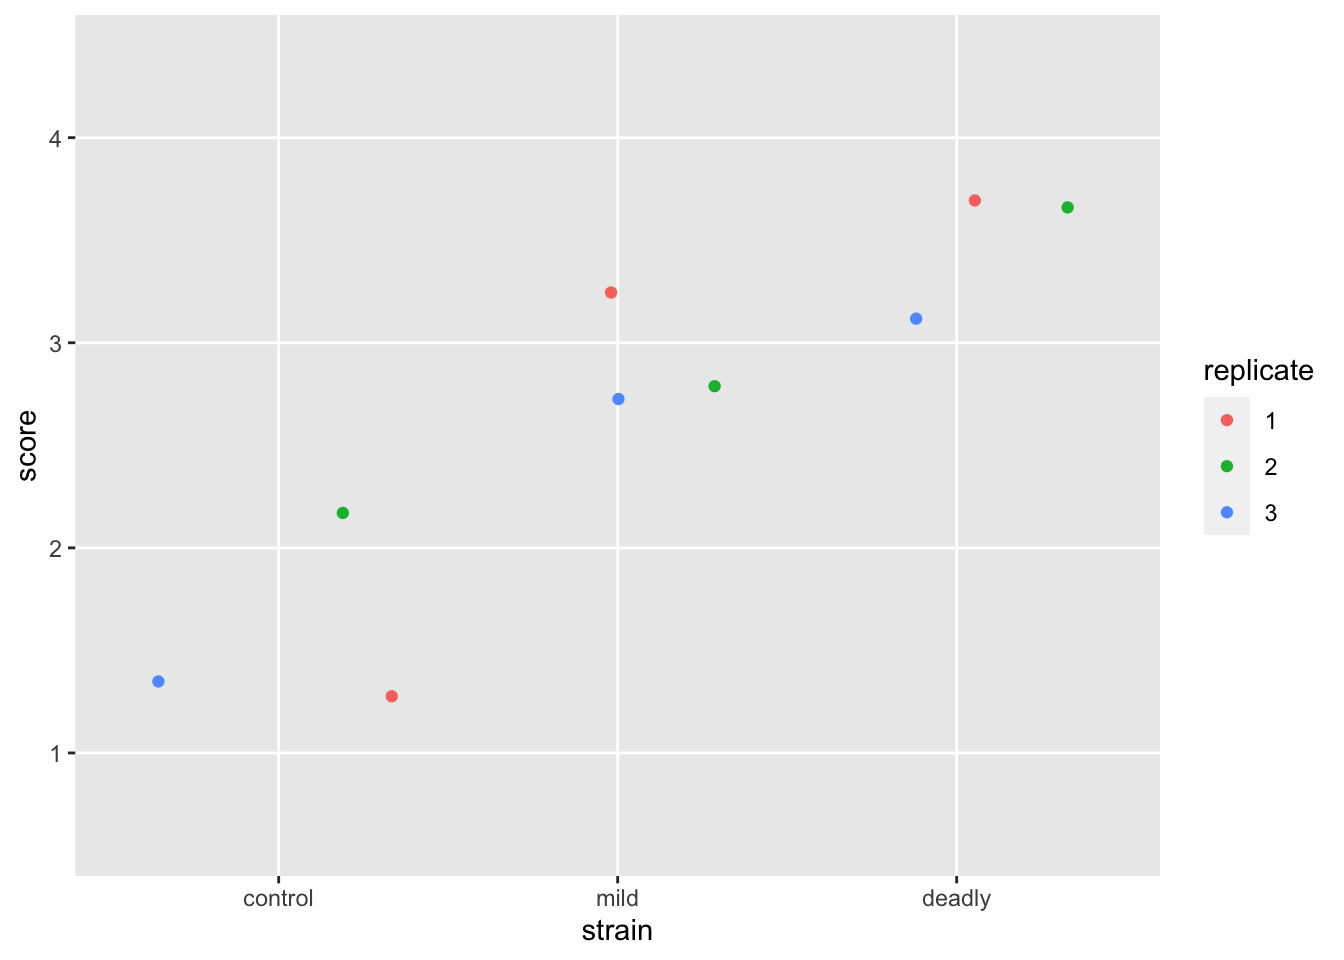
\includegraphics{intro_to_stats_files/figure-latex/unnamed-chunk-107-1.pdf}

Better but not perfect. We get the replicate labelled properly - as discrete categories rather than a continuous scale, and the strain is in a sensible order. But the jitter still leaves us with the impression that we have numeric data. We can fix this but first let's jump to repeating our earlier mistake with boxplots

\begin{Shaded}
\begin{Highlighting}[]
\NormalTok{scores }\OperatorTok\StringTok{ }\KeywordTok{ggplot}\NormalTok{() }\OperatorTok{+}
\StringTok{  }\KeywordTok{aes}\NormalTok{(strain, score) }\OperatorTok{+}
\StringTok{  }\KeywordTok{geom_boxplot}\NormalTok{() }\OperatorTok{+}
\StringTok{  }\KeywordTok{geom_jitter}\NormalTok{(}\KeywordTok{aes}\NormalTok{(}\DataTypeTok{colour =}\NormalTok{ replicate))}
\end{Highlighting}
\end{Shaded}

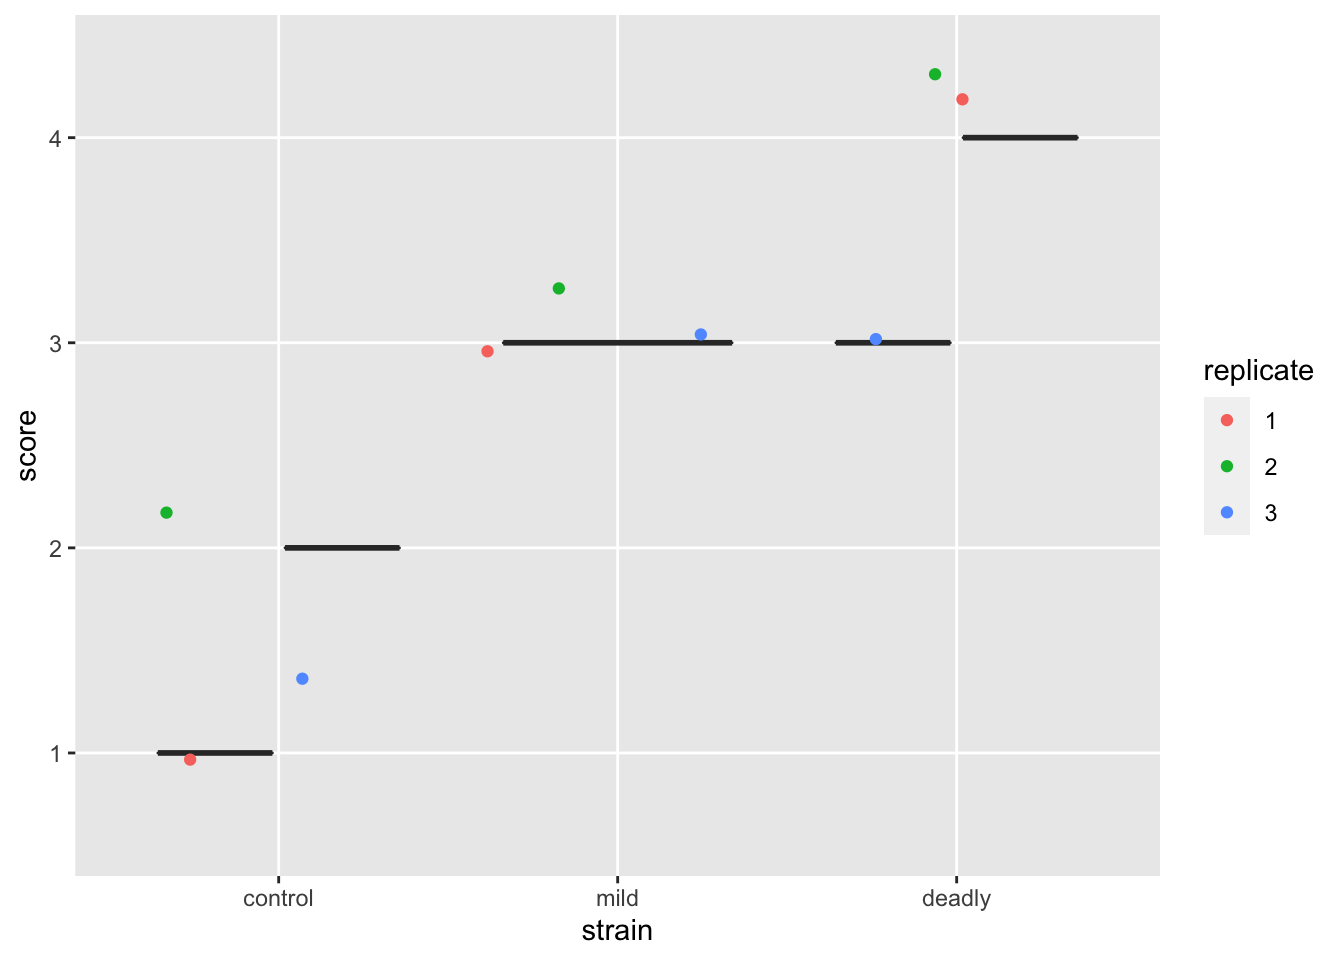
\includegraphics{intro_to_stats_files/figure-latex/unnamed-chunk-108-1.pdf}

OK, weird. The boxplot clearly fails, there isn't the proper data to draw a boxplot, coding our data as factors has saved us this error too. Though not explictly! At least it sends some sort of signal that something isn't right with our plot.

Moving on to evolve our plot, lets remove the jitter and go to a \texttt{geom\_point()} which puts our points in the exact place, without jitter.

\begin{Shaded}
\begin{Highlighting}[]
\NormalTok{scores }\OperatorTok\StringTok{ }\KeywordTok{ggplot}\NormalTok{() }\OperatorTok{+}
\StringTok{  }\KeywordTok{aes}\NormalTok{(strain, score) }\OperatorTok{+}\StringTok{ }
\StringTok{  }\KeywordTok{geom_point}\NormalTok{(}\KeywordTok{aes}\NormalTok{(}\DataTypeTok{colour=}\NormalTok{replicate))}
\end{Highlighting}
\end{Shaded}

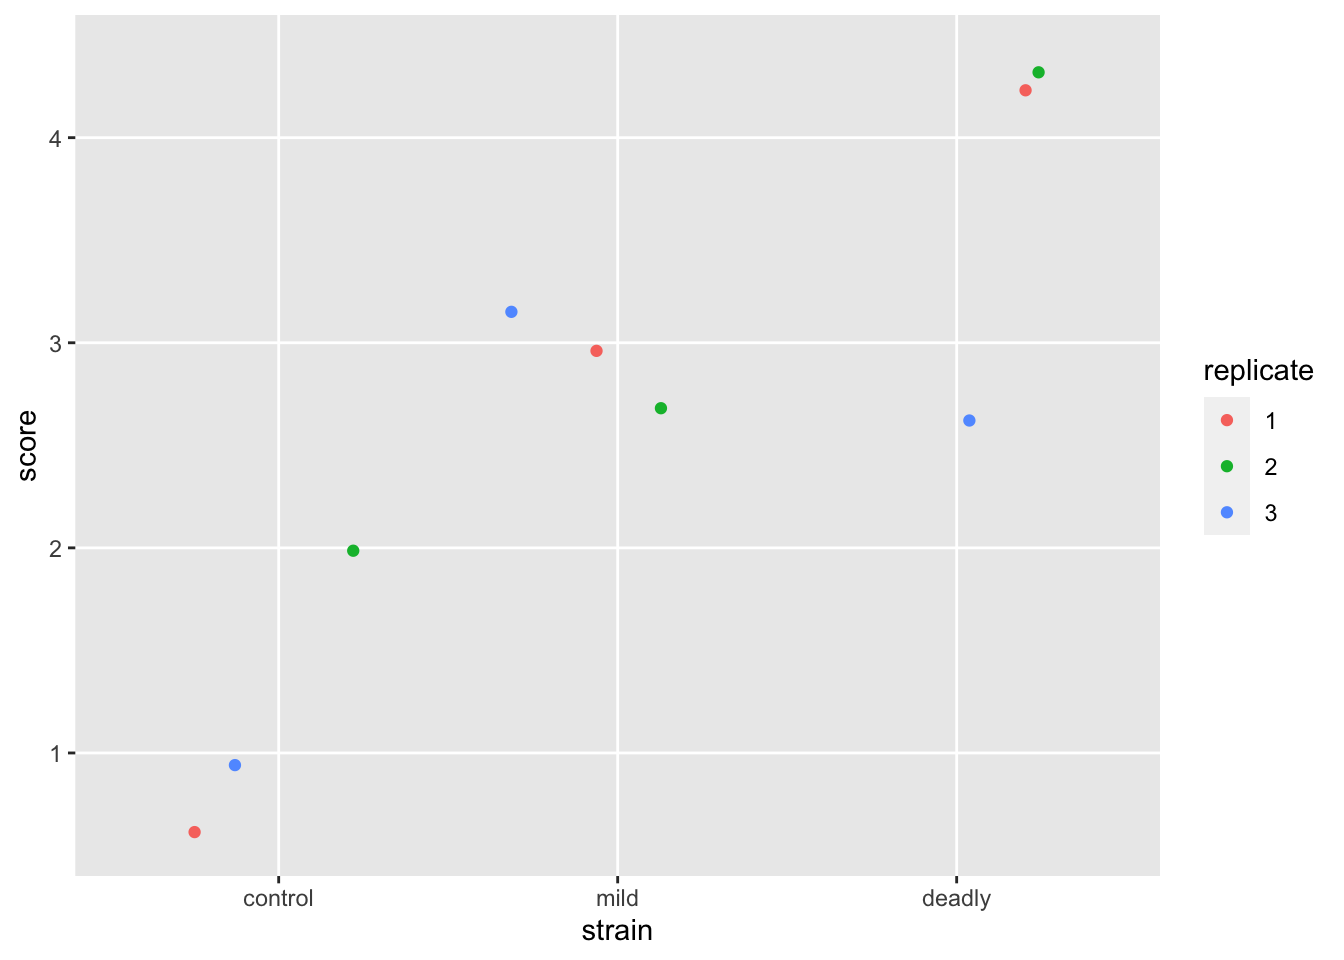
\includegraphics{intro_to_stats_files/figure-latex/unnamed-chunk-109-1.pdf}

this leaves us with the problem that some of our points are overlapped by others. We need a way to show them without moving them off the spot. We can do that by changing the spot size according to the number of points making it up, \texttt{geom\_count()} does that for us.

\begin{Shaded}
\begin{Highlighting}[]
\NormalTok{scores }\OperatorTok\StringTok{ }\KeywordTok{ggplot}\NormalTok{() }\OperatorTok{+}
\StringTok{  }\KeywordTok{aes}\NormalTok{(strain, score) }\OperatorTok{+}\StringTok{ }
\StringTok{  }\KeywordTok{geom_count}\NormalTok{()}
\end{Highlighting}
\end{Shaded}

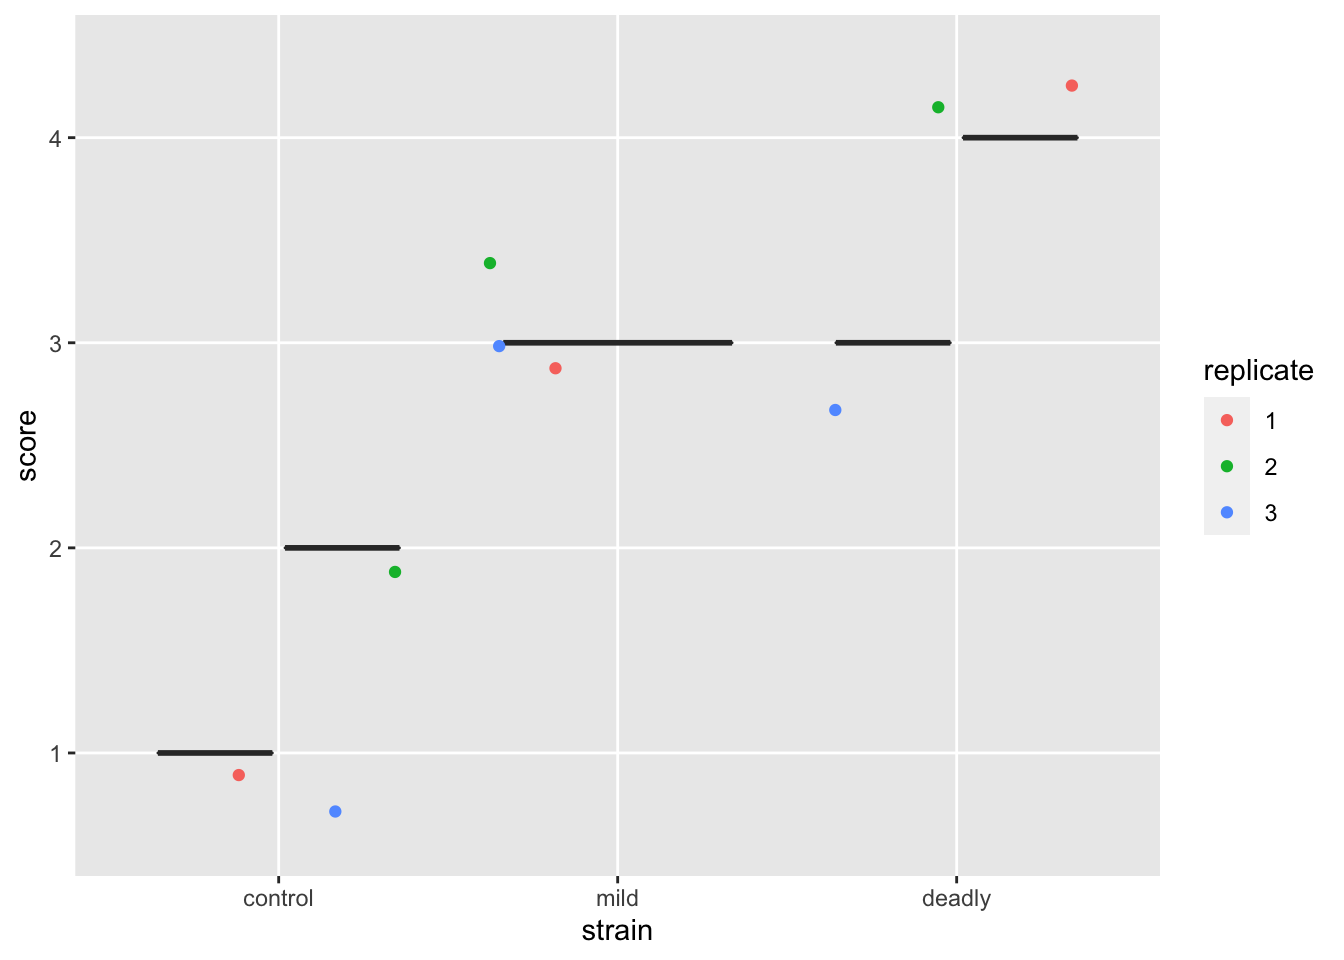
\includegraphics{intro_to_stats_files/figure-latex/unnamed-chunk-110-1.pdf}

And with that we can see the number of datum that make up each point. This is a clearer representation of the categoric data than the early attempts and doesn't lead us to the same poor mental models.

It is possible to get a prettier and more descriptive plot with the different replicates side by side and coloured, but it takes a different set of geoms and a slightly involved approach which has more to do with using \texttt{dplyr} and \texttt{ggplot} so we can leave that as an exercise for another time. The point here is that an appropriate plot for categoric data will save us from a poor understanding of the relationships in the data.

\hypertarget{linear-models-and-a-categoric-y-variable}{%
\section{\texorpdfstring{Linear models and a categoric \(y\) variable}{Linear models and a categoric y variable}}\label{linear-models-and-a-categoric-y-variable}}

After all that exposition about the difference of categories and plotting them properly, how can we apply our knowledge of linear models to find differences between \(x\) categories now that our \(y\) is also categoric and not continuous?

One thing we haven't considered up to now with our categories is that, although categories don't behave like numbers, they can behave like a queue. They often do have an intrinsic and meaningful order. A category like our HR score definitely has an order: \(score\ 1 < score\ 2 < score\ 3 < score\ 4\) even if the intervals are not smooth or equal or defined in any other way. Conversely, some categories don't have an order, e.g species 1 and species 2 aren't greater or lesser than each other. We need to treat ordered and unordered categories differently.

\hypertarget{ordered-categoric-response-variables}{%
\subsection{Ordered categoric response variables}\label{ordered-categoric-response-variables}}

The steps for working with an ordered categoric response variable are as follows

\begin{enumerate}
\def\labelenumi{\arabic{enumi}.}
\tightlist
\item
  Convert the values observed in the ordered categoric response variable to a rank
\item
  Proceed as before
\end{enumerate}

It's that easy! Ranks are continuous and work as if they were a continuous scale, so we can use them as we did before. Let's look at how to rank an ordered categoric variable

The first step is to tell R that the factor is in fact an ordered one, and what that order is

\begin{Shaded}
\begin{Highlighting}[]
\NormalTok{observations <-}\StringTok{ }\KeywordTok{c}\NormalTok{(}\StringTok{"none"}\NormalTok{, }\StringTok{"some"}\NormalTok{, }\StringTok{"some"}\NormalTok{, }\StringTok{"none"}\NormalTok{, }\StringTok{"lots"}\NormalTok{, }\StringTok{"many"}\NormalTok{)}

\NormalTok{ordfac_observations <-}\StringTok{ }\KeywordTok{factor}\NormalTok{(observations, }
                          \DataTypeTok{levels =} \KeywordTok{c}\NormalTok{(}\StringTok{"none"}\NormalTok{, }\StringTok{"some"}\NormalTok{, }\StringTok{"many"}\NormalTok{, }\StringTok{"lots"}\NormalTok{, }\StringTok{"all"}\NormalTok{),}
                          \DataTypeTok{ordered =} \OtherTok{TRUE}
\NormalTok{                          )}
\end{Highlighting}
\end{Shaded}

All we've done here is create some data in \texttt{observations} then turn it into a factor, the \texttt{levels} option sets the allowed levels and the \texttt{ordered} option tells R to take the given order. Let's inspect the factor object by printing

\begin{Shaded}
\begin{Highlighting}[]
\NormalTok{ordfac_observations}
\end{Highlighting}
\end{Shaded}

\begin{verbatim}
## [1] none some some none lots many
## Levels: none < some < many < lots < all
\end{verbatim}

We see that R knows the data and the order of the levels. Note that even if a level doesn't appear in the data, as long as it is declared in \texttt{levels} R still knows about it and it's place, should it come across it.

We can convert to a rank quite easily with the \texttt{rank()} function.

\begin{Shaded}
\begin{Highlighting}[]
\KeywordTok{rank}\NormalTok{(ordfac_observations)}
\end{Highlighting}
\end{Shaded}

\begin{verbatim}
## [1] 1.5 3.5 3.5 1.5 6.0 5.0
\end{verbatim}

And R converts our category to a rank based on the order we provided. Note that ties are broken, so the two \texttt{nones} get equal but split rank, as do the two \texttt{somes}. This operation gives us a numeric scale we can use as if the data were continuous.

\hypertarget{making-linear-models-with-ranked-data}{%
\subsection{Making linear models with ranked data}\label{making-linear-models-with-ranked-data}}

Let's calculate the rank score and add it to the score data frame with \texttt{transmute()}, then plot the rank data.

\begin{Shaded}
\begin{Highlighting}[]
\NormalTok{scores <-}\StringTok{ }\NormalTok{scores }\OperatorTok\StringTok{ }\KeywordTok{transmute}\NormalTok{(}
  \DataTypeTok{score =} \KeywordTok{factor}\NormalTok{(score, }\DataTypeTok{levels =} \KeywordTok{c}\NormalTok{(}\StringTok{"1"}\NormalTok{,}\StringTok{"2"}\NormalTok{,}\StringTok{"3"}\NormalTok{,}\StringTok{"4"}\NormalTok{), }\DataTypeTok{ordered =} \OtherTok{TRUE}\NormalTok{),}
  \DataTypeTok{rank_score =} \KeywordTok{rank}\NormalTok{(score),}
\NormalTok{  strain,replicate}
\NormalTok{)}

\KeywordTok{ggplot}\NormalTok{(scores) }\OperatorTok{+}\StringTok{ }\KeywordTok{aes}\NormalTok{(strain, rank_score) }\OperatorTok{+}\StringTok{ }\KeywordTok{geom_jitter}\NormalTok{(}\KeywordTok{aes}\NormalTok{(}\DataTypeTok{colour =}\NormalTok{ replicate))}
\end{Highlighting}
\end{Shaded}

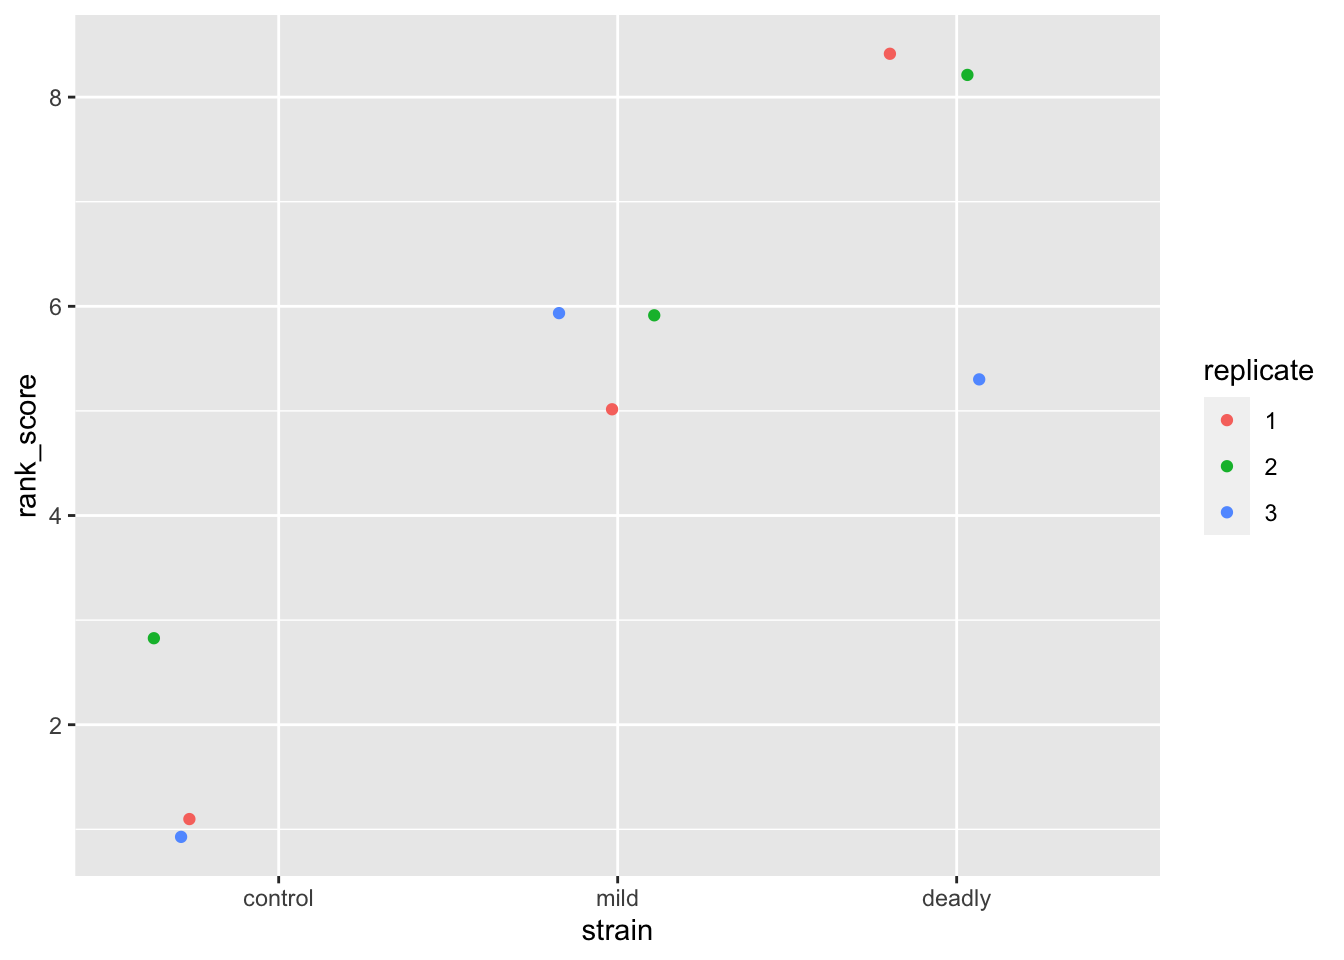
\includegraphics{intro_to_stats_files/figure-latex/unnamed-chunk-114-1.pdf}

We can see the ranks and replicates in the scatter plot that we are used to, we have a similar view as to that we saw with the categoric scatter plot.

Now we can move on to the modelling and the ANOVA

\begin{Shaded}
\begin{Highlighting}[]
\NormalTok{model <-}\StringTok{ }\KeywordTok{lm}\NormalTok{(rank_score }\OperatorTok{~}\StringTok{ }\NormalTok{strain, }\DataTypeTok{data =}\NormalTok{ scores)}
\KeywordTok{summary}\NormalTok{(model)}
\end{Highlighting}
\end{Shaded}

\begin{verbatim}
## 
## Call:
## lm(formula = rank_score ~ strain, data = scores)
## 
## Residuals:
##    Min     1Q Median     3Q    Max 
##   -2.0   -0.5    0.0    1.0    1.0 
## 
## Coefficients:
##              Estimate Std. Error t value Pr(>|t|)    
## (Intercept)    2.0000     0.6455   3.098 0.021160 *  
## strainmild     3.5000     0.9129   3.834 0.008618 ** 
## straindeadly   5.5000     0.9129   6.025 0.000944 ***
## ---
## Signif. codes:  0 '***' 0.001 '**' 0.01 '*' 0.05 '.' 0.1 ' ' 1
## 
## Residual standard error: 1.118 on 6 degrees of freedom
## Multiple R-squared:  0.8611,	Adjusted R-squared:  0.8148 
## F-statistic:  18.6 on 2 and 6 DF,  p-value: 0.002679
\end{verbatim}

\begin{Shaded}
\begin{Highlighting}[]
\KeywordTok{library}\NormalTok{(multcomp)}
\KeywordTok{summary}\NormalTok{(}\KeywordTok{glht}\NormalTok{(}
\NormalTok{  model, }\DataTypeTok{linfct =} \KeywordTok{mcp}\NormalTok{(}\DataTypeTok{strain =} \StringTok{"Tukey"}\NormalTok{)}
\NormalTok{))}
\end{Highlighting}
\end{Shaded}

\begin{verbatim}
## 
## 	 Simultaneous Tests for General Linear Hypotheses
## 
## Multiple Comparisons of Means: Tukey Contrasts
## 
## 
## Fit: lm(formula = rank_score ~ strain, data = scores)
## 
## Linear Hypotheses:
##                       Estimate Std. Error t value Pr(>|t|)   
## mild - control == 0     3.5000     0.9129   3.834  0.02030 * 
## deadly - control == 0   5.5000     0.9129   6.025  0.00196 **
## deadly - mild == 0      2.0000     0.9129   2.191  0.15142   
## ---
## Signif. codes:  0 '***' 0.001 '**' 0.01 '*' 0.05 '.' 0.1 ' ' 1
## (Adjusted p values reported -- single-step method)
\end{verbatim}

Great, some clear answers. The strains are likely not the same as the control, but there is no evidence for difference between the strains.

\hypertarget{hypothesis-tests}{%
\section{Hypothesis Tests}\label{hypothesis-tests}}

As we mentioned at the start of the chapter there are hypothesis tests that we can use instead of the linear model approach for the ordered categoric response variable case. These are the Mann-Whitney U test (also called the Wilcoxon Signed Rank test) which is for a two group situation (like a \(t\)-test) and the Kruskal-Wallis test, which is for a multi-group situation (like the ANOVA).

However, we run into some problems when doing these tests, especially for multiple categories. The Mann-Whitney U only works on two groups, which is a limitation. It is used as below, though first we'll need to extract the two groups we want. We will do this by filtering but then we'll need to extract any unused levels in the filtered factor \texttt{strain} with \texttt{droplevels()}

\begin{Shaded}
\begin{Highlighting}[]
\KeywordTok{library}\NormalTok{(dplyr)}
\NormalTok{two_groups <-}\StringTok{ }\KeywordTok{filter}\NormalTok{(scores, strain }\OperatorTok{!=}\StringTok{ "deadly"}\NormalTok{) }\OperatorTok\StringTok{ }
\StringTok{  }\KeywordTok{droplevels}\NormalTok{() }\OperatorTok\StringTok{ }
\StringTok{  }\KeywordTok{transmute}\NormalTok{(}\DataTypeTok{score =} \KeywordTok{as.numeric}\NormalTok{(}\KeywordTok{as.character}\NormalTok{(score)),}
\NormalTok{            strain, replicate}
\NormalTok{            )}

\KeywordTok{str}\NormalTok{(two_groups)}
\end{Highlighting}
\end{Shaded}

\begin{verbatim}
## tibble [6 x 3] (S3: tbl_df/tbl/data.frame)
##  $ score    : num [1:6] 1 3 2 3 1 3
##  $ strain   : Factor w/ 2 levels "control","mild": 1 2 1 2 1 2
##  $ replicate: Factor w/ 3 levels "1","2","3": 1 1 2 2 3 3
\end{verbatim}

\begin{Shaded}
\begin{Highlighting}[]
\KeywordTok{wilcox.test}\NormalTok{(score }\OperatorTok{~}\StringTok{ }\NormalTok{strain, }\DataTypeTok{data =}\NormalTok{ two_groups)}
\end{Highlighting}
\end{Shaded}

\begin{verbatim}
## Warning in wilcox.test.default(x = c(1, 2, 1), y = c(3, 3, 3)): cannot compute
## exact p-value with ties
\end{verbatim}

\begin{verbatim}
## 
## 	Wilcoxon rank sum test with continuity correction
## 
## data:  score by strain
## W = 0, p-value = 0.05935
## alternative hypothesis: true location shift is not equal to 0
\end{verbatim}

So the Mann-Whitney U (Wilcoxon) test tells us that the difference between the scores between the two strains is not likely to be 0. Scaling this up to more than two groups takes a Kruskal-Wallis test

\begin{Shaded}
\begin{Highlighting}[]
\KeywordTok{kruskal.test}\NormalTok{(rank_score }\OperatorTok{~}\StringTok{ }\NormalTok{strain, }\DataTypeTok{data =}\NormalTok{ scores)}
\end{Highlighting}
\end{Shaded}

\begin{verbatim}
## 
## 	Kruskal-Wallis rank sum test
## 
## data:  rank_score by strain
## Kruskal-Wallis chi-squared = 6.8889, df = 2, p-value = 0.03192
\end{verbatim}

Now this is disappointing, as the Kruskal-Wallis test tells us that at least one of the groups is different from the others, but crucially it doesn't tell us which ones! So we end up doing a multiple \texttt{wilcox.test()} and applying a correction to the \(p\)-value. The linear model and ANOVA approach, proves to be a little more straightforward now that we have the knack.

\hypertarget{but-arent-the-tests-just-easier}{%
\subsection{But aren't the tests just easier?}\label{but-arent-the-tests-just-easier}}

As with the \(t\)-test, then in practice, sometimes, yes, these tests are easier. But the same reason for using the linear model applies as with the \(t\)-test - it gives us a general framework in which to work and develop a good intuition about the data we are studying and a good conceptual tool with which to think about it. As ever the individual hypothesis tests are just easier. But as we've seen they run into limitations of their own.

\begin{roundup}
\begin{itemize}
\tightlist
\item
  It is easy to mistake categories for continuous data when numbers are use as names.

  \begin{itemize}
  \tightlist
  \item
    Using numbers as names does not make data quantitative
  \item
    Ranking data makes it possible to analyse ordered categoric data in a linear model
  \end{itemize}
\end{itemize}
\end{roundup}

\begin{task}
\end{task}

\hypertarget{chi-2-tests-and-linear-models}{%
\chapter{\texorpdfstring{\(\chi ^2\) tests and linear models}{\textbackslash chi \^{}2 tests and linear models}}\label{chi-2-tests-and-linear-models}}

\begin{enumerate}
\def\labelenumi{\arabic{enumi}.}
\tightlist
\item
  Questions
\end{enumerate}

\begin{itemize}
\tightlist
\item
  How do linear models apply when both the \(x\) and \(y\) are not continuous?
\item
  How can I analyse counts of stuff?
\end{itemize}

\begin{enumerate}
\def\labelenumi{\arabic{enumi}.}
\setcounter{enumi}{1}
\tightlist
\item
  Objectives
\end{enumerate}

\begin{itemize}
\tightlist
\item
  Appreciate that the linear model idea does not translate intuitively to this data
\item
  Learn how to do a \(\chi^2\) test for a given number of variables
\end{itemize}

\begin{enumerate}
\def\labelenumi{\arabic{enumi}.}
\setcounter{enumi}{2}
\tightlist
\item
  Keypoints
\end{enumerate}

\begin{itemize}
\tightlist
\item
  Linear models applied in the place of \(\chi^2\) tests are fiddly and in practice we are usually better off using the hypothesis tests
\end{itemize}

In the last chapter we looked at discrete data that was ordered and got around it, as hypothesis tests do, by working on ranked data with a linear model. In this section we'll look at discrete data that isn't ordered, or is nominal, things like \texttt{agree,\ disagree,\ don\textquotesingle{}t\ know}, or \texttt{yellow,\ green,\ wrinkled,\ smooth}. We'll also look at discrete data in the form of counts or frequencies.

\hypertarget{the-problem-with-unordered-response-data}{%
\section{The problem with unordered response data}\label{the-problem-with-unordered-response-data}}

If we have unordered categoric response data (\(y\)-axis) we find ourselves in a bit of a pickle if we want to try to apply a linear model to understand relationships, because there are no numbers \emph{at all}. In every other example we've looked at the \(y\) response data has been numeric or at least coercible into numbers.

We'll put ourselves in the shoes of Gregor Mendel and work through his monohybrid cross experiment on flower colour. Mendel's first step would have been to work out the flower colours after a cross with different coloured true breeding parents, leaving him with a raw dataframe like this:

\begin{Shaded}
\begin{Highlighting}[]
\KeywordTok{library}\NormalTok{(itssl)}
\KeywordTok{its_mendel_data_time}\NormalTok{()}
\end{Highlighting}
\end{Shaded}

\begin{verbatim}
## # A tibble: 600 x 2
##    cross result
##    <chr> <chr> 
##  1 WP    P     
##  2 WP    P     
##  3 WP    P     
##  4 PW    P     
##  5 WP    P     
##  6 PW    P     
##  7 PW    P     
##  8 PW    P     
##  9 WP    P     
## 10 PP    P     
## # ... with 590 more rows
\end{verbatim}

Which isn't very helpful at this stage, how on earth do we get two columns of text into a linear model? Persevering, Mendel would've gone on to count the numbers of each colour.

\begin{Shaded}
\begin{Highlighting}[]
\KeywordTok{its_mendel_count_data_time}\NormalTok{()}
\end{Highlighting}
\end{Shaded}

\begin{verbatim}
## # A tibble: 2 x 2
##   colour count
##   <chr>  <int>
## 1 P        459
## 2 W        141
\end{verbatim}

Mendel famously went on to calculate the ratios, or relative frequencies of each.

\begin{Shaded}
\begin{Highlighting}[]
\KeywordTok{its_mendel_frequency_time}\NormalTok{()}
\end{Highlighting}
\end{Shaded}

\begin{verbatim}
## # A tibble: 1 x 6
##       P     W ratio_p ratio_w freq_p freq_w
##   <int> <int>   <dbl>   <dbl>  <dbl>  <dbl>
## 1   459   141    3.26       1  0.765  0.235
\end{verbatim}

But that doesn't get us any nearer. The problem is that we have just got count (or frequency) data and nothing else. It seems that it isn't far from the ordered data case, we can imagine plotting the data as we did with HR score, but the response variable is colour and there's no clear explanatory (\(x\)) variable, so what would go on that axis? Perhaps the colour of the parents in the cross as categories would do? There isn't an order to this so we can't meaningfully apply the rank to create a proxy for order. We can't look at slopes again because there's no sense in the order of the response variable. In short it's a mess.

\begin{sidenote}
Why isn't colour an explanatory variable? And why can't then frequency or count be the \(y\)-axis? Well, at a push they sort of might nearly be. But maybe not really. Remember the values of an explanatory variable should be something we can change as an experimenter, they are the values that we change deliberately to see what the effect on the response is. Even in our categoric \(x\)-experiments we know what the values will be beforehand. Here, arguably we didn't, crosses happened and phenotypes popped out, so it's a bit muddier. If we do use that approach we end up with lots of observations condensed into one number as a further issue.
\end{sidenote}

\hypertarget{we-have-to-compare-models-not-groups.}{%
\section{We have to compare models, not groups.}\label{we-have-to-compare-models-not-groups.}}

It is possible to do this sort of comparison with linear models, but it gets to be fiddly and involved because we need to apply a mathematical transformation to our counts and to work on the likelihood ratio of the response to stick to some assumptions of the modelling process.

Briefly we go from this linear model, with interaction terms

\begin{verbatim}
y ~ a + b + c + a:b
\end{verbatim}

To two models with logs all over them, one with interaction terms, one without

\begin{verbatim}
log(yi) ~ log(N) + log(ai) + log(bi) + log(ci) + log(aibi)
log(yi) ~ log(N) + log(ai) + log(bi) + log(ci)
\end{verbatim}

And then we have to compare the models to see which fit the data best.

Which is more complicated than we want to get into and ultimately the process is not worth it in most cases, because there are alternatives. Pragmatically, the answer is to use the \(\chi^2\) and related tests in this case.

It is worthwhile to remember that to analyse unordered categoric response data we need to compare models, because that means assessing which model `fit' the data we have best. This is a useful way to think about what the tests like the \(\chi^2\) and Fisher's Exact test are doing. They compare the observed counts - being considered one full set of data (or one model), against the expected counts from some ideal or some category split, a second model.

The log-linear model and the tests give closely equivalent results in most cases.

\hypertarget{the-chi2-test}{%
\section{\texorpdfstring{The \(\chi^2\) test}{The \textbackslash chi\^{}2 test}}\label{the-chi2-test}}

In the \(\chi^2\) test we ask `does one set of counts differ from another?'. This might be a hypothetical `expected' set of counts for the response of interest compared to some standard.
For example, in genetics data we might ask whether the observed ratio of phenotypes matches an expected \texttt{9:3:3:1}. More generally, we might ask whether the counts in one subset of categories matches another, so in a survey to ask whether respondents agree that broccoli is a nice food, with response `agree, disagree, don't know', we might compare responses between adults and children.

The basic calculation in the \(\chi^2\) test is the difference between observed and expected numbers in each category subset. In Mendel's data this would be the difference between the observed number of ``P'' and ``W'', from the expected number - given we did 600 plants, then for a \(3:1\) we'd expect 450 ``P'' and 150 ``W''. This difference is then compared to values of the dev\(\chi^2\) distribution and returns a \(p\)-value that represents how far away from the mean the difference is. If it is an extreme value (in the tails) the \(p\)-value is lower.

The hypotheses are set as follows:

\begin{itemize}
\tightlist
\item
  \(H_{0}\) the observed counts show no evidence that they are different from the expected counts
\item
  \(H_{1}\) the observed counts would not occur often by chance
\end{itemize}

\hypertarget{performing-the-test}{%
\subsection{Performing the test}\label{performing-the-test}}

To do the test for the simplest case - Mendel's flower data, we need to get a dataframe with the observed counts on one row and the expected counts on another.

\begin{Shaded}
\begin{Highlighting}[]
\NormalTok{observed_counts <-}\StringTok{ }\KeywordTok{its_mendel_count_data_time}\NormalTok{() }\OperatorTok\StringTok{ }
\StringTok{  }\NormalTok{tidyr}\OperatorTok{::}\KeywordTok{pivot_wider}\NormalTok{(}\DataTypeTok{names_from =} \KeywordTok{c}\NormalTok{(}\StringTok{"colour"}\NormalTok{), }\DataTypeTok{values_from =} \KeywordTok{c}\NormalTok{(}\StringTok{"count"}\NormalTok{) )}
\NormalTok{observed_counts}
\end{Highlighting}
\end{Shaded}

\begin{verbatim}
## # A tibble: 1 x 2
##       P     W
##   <int> <int>
## 1   459   141
\end{verbatim}

We then need to make the equivalent row for the expected counts - recall we had 600 plants, so calculate the expected number of ``P'' and ``W''

\begin{Shaded}
\begin{Highlighting}[]
\NormalTok{expected_counts <-}\StringTok{ }\NormalTok{tibble}\OperatorTok{::}\KeywordTok{tibble}\NormalTok{(}
   \DataTypeTok{P =} \DecValTok{600} \OperatorTok{*}\StringTok{ }\DecValTok{3}\OperatorTok{/}\DecValTok{4}\NormalTok{,}
   \DataTypeTok{W =}  \DecValTok{600} \OperatorTok{*}\StringTok{ }\DecValTok{1}\OperatorTok{/}\DecValTok{4}
\NormalTok{)}
\NormalTok{expected_counts}
\end{Highlighting}
\end{Shaded}

\begin{verbatim}
## # A tibble: 1 x 2
##       P     W
##   <dbl> <dbl>
## 1   450   150
\end{verbatim}

We then need to stick those rows together

\begin{Shaded}
\begin{Highlighting}[]
\NormalTok{chi_sq_input <-}\StringTok{ }\NormalTok{dplyr}\OperatorTok{::}\KeywordTok{bind_rows}\NormalTok{(observed_counts, expected_counts)}
\KeywordTok{rownames}\NormalTok{(chi_sq_input) <-}\StringTok{ }\KeywordTok{c}\NormalTok{(}\StringTok{"observed"}\NormalTok{, }\StringTok{"expected"}\NormalTok{)}
\end{Highlighting}
\end{Shaded}

\begin{verbatim}
## Warning: Setting row names on a tibble is deprecated.
\end{verbatim}

\begin{Shaded}
\begin{Highlighting}[]
\NormalTok{chi_sq_input}
\end{Highlighting}
\end{Shaded}

\begin{verbatim}
## # A tibble: 2 x 2
##       P     W
## * <dbl> <dbl>
## 1   459   141
## 2   450   150
\end{verbatim}

Finally we can do the test with the function \texttt{chisq.test()}

\begin{Shaded}
\begin{Highlighting}[]
\KeywordTok{chisq.test}\NormalTok{(chi_sq_input)}
\end{Highlighting}
\end{Shaded}

\begin{verbatim}
## 
## 	Pearson's Chi-squared test with Yates' continuity correction
## 
## data:  chi_sq_input
## X-squared = 0.29034, df = 1, p-value = 0.59
\end{verbatim}

The test shows us that the \(p\)-value of the \(\chi^2\) test is greater than 0.05 so we conclude that there is no evidence that the observed number of each flower colour differs from the expected and that we do indeed have a \(3:1\) ratio. Note that the test automatically does the necessary correction for small sample sizes if the data need it.

\hypertarget{more-than-one-variable}{%
\subsection{More than one variable}\label{more-than-one-variable}}

The data we had above only had one variable, flower colour. What if we have multiple categoric variables to compare? Largely, the process is the same but making the table is more difficult.

Consider this data frame of voting intentions between generations

\begin{Shaded}
\begin{Highlighting}[]
\CommentTok{##Turn into function in the package}
\NormalTok{voting_data <-}\StringTok{ }\KeywordTok{its_voting_data_time}\NormalTok{()}
\NormalTok{voting_data}
\end{Highlighting}
\end{Shaded}

\begin{verbatim}
##   generation alignment count
## 1     boomer   fascist   279
## 2  millenial   fascist   165
## 3     boomer instagram    74
## 4  millenial instagram    47
## 5     boomer   marxist   225
## 6  millenial   marxist   191
\end{verbatim}

This time we have two variables, with two or three levels of each. To make the contingency table for \texttt{chisq.test()} we can use \texttt{xtabs()} which takes an R formula as a description of how to make the table. Luckily, these are exactly the same formula we used to make linear models.

\begin{Shaded}
\begin{Highlighting}[]
\NormalTok{tabulated <-}\StringTok{ }\KeywordTok{xtabs}\NormalTok{(count }\OperatorTok{~}\StringTok{ }\NormalTok{., }\DataTypeTok{data =}\NormalTok{ voting_data)}
\NormalTok{tabulated}
\end{Highlighting}
\end{Shaded}

\begin{verbatim}
##            alignment
## generation  fascist instagram marxist
##   boomer        279        74     225
##   millenial     165        47     191
\end{verbatim}

Here we make a formula that says \texttt{count} is the output variable, and \texttt{.} are the independent or row and column variables (\texttt{.} in formula like this just means everything else). The table comes out as we expect and we can go on to do the \texttt{chisq.test()} as before on the new table.

\begin{Shaded}
\begin{Highlighting}[]
\KeywordTok{chisq.test}\NormalTok{(tabulated)}
\end{Highlighting}
\end{Shaded}

\begin{verbatim}
## 
## 	Pearson's Chi-squared test
## 
## data:  tabulated
## X-squared = 7.0811, df = 2, p-value = 0.029
\end{verbatim}

Here the \(p\) value tells us that the pattern of voting intention is significant, but the numbers are hard to interpret \ldots{} do \texttt{millenial}s vote less for \texttt{instagram} than \texttt{boomer}s? We can make things easier to interpret if we have a proportion table. The function \texttt{prop.table()} can make one of those.

\begin{Shaded}
\begin{Highlighting}[]
\KeywordTok{prop.table}\NormalTok{(tabulated, }\DataTypeTok{margin =} \DecValTok{1}\NormalTok{)}
\end{Highlighting}
\end{Shaded}

\begin{verbatim}
##            alignment
## generation    fascist instagram   marxist
##   boomer    0.4826990 0.1280277 0.3892734
##   millenial 0.4094293 0.1166253 0.4739454
\end{verbatim}

The \texttt{margin} option takes a \texttt{1} if we want proportions across the rows, \texttt{2} if we want proportions down the columns. We can see that the difference between the two generations comes largely from a swing from \texttt{fascist} to \texttt{marxist}.

\hypertarget{more-than-one-pairwise-comparison}{%
\subsection{More than one pairwise comparison}\label{more-than-one-pairwise-comparison}}

If we have more than two levels in our comparison category (that is, a larger contingency table than 2 x 2), we run into a problem. Look at these data

\begin{Shaded}
\begin{Highlighting}[]
\NormalTok{job_mood <-}\StringTok{ }\KeywordTok{its_job_mood_time}\NormalTok{()}
\end{Highlighting}
\end{Shaded}

\begin{Shaded}
\begin{Highlighting}[]
\NormalTok{tab <-}\StringTok{ }\KeywordTok{xtabs}\NormalTok{(Freq }\OperatorTok{~}\NormalTok{., }\DataTypeTok{data =}\NormalTok{ job_mood)}
\NormalTok{tab}
\end{Highlighting}
\end{Shaded}

\begin{verbatim}
##            role
## mood        carpenter cooper milliner
##   curious          70      0      100
##   tense            32     30       30
##   whimsical       120    142      110
\end{verbatim}

we have data on the reported mood of people in different jobs. Note that there are three levels of each of the categoric variables. We can make the table and can go straight to the \(\chi^2\) test.

\begin{Shaded}
\begin{Highlighting}[]
\NormalTok{tab <-}\StringTok{ }\KeywordTok{xtabs}\NormalTok{(Freq }\OperatorTok{~}\NormalTok{., }\DataTypeTok{data =}\NormalTok{ job_mood)}
\NormalTok{tab}
\end{Highlighting}
\end{Shaded}

\begin{verbatim}
##            role
## mood        carpenter cooper milliner
##   curious          70      0      100
##   tense            32     30       30
##   whimsical       120    142      110
\end{verbatim}

\begin{Shaded}
\begin{Highlighting}[]
\KeywordTok{chisq.test}\NormalTok{(tab)}
\end{Highlighting}
\end{Shaded}

\begin{verbatim}
## 
## 	Pearson's Chi-squared test
## 
## data:  tab
## X-squared = 93.67, df = 4, p-value < 2.2e-16
\end{verbatim}

Umm, it's significant. But weren't we expecting to see significances between groups? As with the ANOVA it's done the overall result. We need to do a \emph{post-hoc} operation to do the full set of pairwise comparisons. The package \texttt{rcompanion} has a nice function for this, \texttt{pairwiseNominalIndependence()}, we set the option \texttt{method} to decide which correction for multiple comparisons to do, \texttt{fdr} is a good choice.

\begin{Shaded}
\begin{Highlighting}[]
\KeywordTok{library}\NormalTok{(rcompanion)}
\KeywordTok{pairwiseNominalIndependence}\NormalTok{(tab, }\DataTypeTok{method =} \StringTok{"fdr"}\NormalTok{)}
\end{Highlighting}
\end{Shaded}

\begin{verbatim}
##            Comparison p.Fisher p.adj.Fisher  p.Gtest p.adj.Gtest  p.Chisq
## 1     curious : tense 8.97e-16     1.35e-15 2.22e-16    3.33e-16 1.07e-14
## 2 curious : whimsical 8.98e-29     2.69e-28 0.00e+00    0.00e+00 5.47e-21
## 3   tense : whimsical 5.98e-01     5.98e-01 6.07e-01    6.07e-01 6.11e-01
##   p.adj.Chisq
## 1    1.60e-14
## 2    1.64e-20
## 3    6.11e-01
\end{verbatim}

Better. But not quite! The groups compared are the different \texttt{moods}, presumably we wanted to look at the differences between the different \texttt{roles}. The table is in the wrong orientation in that case.

We can explicitly state the orientation of the table by manipulating the formula in \texttt{xtabs()}. Compare the results of these two calls

\begin{Shaded}
\begin{Highlighting}[]
\KeywordTok{xtabs}\NormalTok{(Freq }\OperatorTok{~}\StringTok{ }\NormalTok{role }\OperatorTok{+}\StringTok{ }\NormalTok{mood, }\DataTypeTok{data =}\NormalTok{ job_mood)}
\end{Highlighting}
\end{Shaded}

\begin{verbatim}
##            mood
## role        curious tense whimsical
##   carpenter      70    32       120
##   cooper          0    30       142
##   milliner      100    30       110
\end{verbatim}

\begin{Shaded}
\begin{Highlighting}[]
\KeywordTok{xtabs}\NormalTok{(Freq }\OperatorTok{~}\StringTok{ }\NormalTok{mood }\OperatorTok{+}\StringTok{ }\NormalTok{role, }\DataTypeTok{data =}\NormalTok{ job_mood)}
\end{Highlighting}
\end{Shaded}

\begin{verbatim}
##            role
## mood        carpenter cooper milliner
##   curious          70      0      100
##   tense            32     30       30
##   whimsical       120    142      110
\end{verbatim}

We usually want the form with the variable we're comparing in the rows, that's the \texttt{Freq\ \textasciitilde{}\ role\ +\ mood}. We can then do the pairwise \(\chi^2\).

\begin{Shaded}
\begin{Highlighting}[]
\NormalTok{tab <-}\StringTok{ }\KeywordTok{xtabs}\NormalTok{(Freq }\OperatorTok{~}\StringTok{ }\NormalTok{role }\OperatorTok{+}\StringTok{ }\NormalTok{mood, }\DataTypeTok{data =}\NormalTok{ job_mood)}
\KeywordTok{pairwiseNominalIndependence}\NormalTok{(tab, }\DataTypeTok{method =} \StringTok{"fdr"}\NormalTok{)}
\end{Highlighting}
\end{Shaded}

\begin{verbatim}
##             Comparison p.Fisher p.adj.Fisher p.Gtest p.adj.Gtest  p.Chisq
## 1   carpenter : cooper 5.26e-20     7.89e-20  0.0000      0.0000 3.38e-15
## 2 carpenter : milliner 7.81e-02     7.81e-02  0.0773      0.0773 7.81e-02
## 3    cooper : milliner 1.66e-28     4.98e-28  0.0000      0.0000 1.89e-21
##   p.adj.Chisq
## 1    5.07e-15
## 2    7.81e-02
## 3    5.67e-21
\end{verbatim}

And we can now clearly see the \(p\)-values across all the group comparisons. The default output is actually from a range of \(\chi^2\) related tests. In this case always take the \texttt{p.adj} value as the final \(p\)-value.

\hypertarget{summary}{%
\section{Summary}\label{summary}}

We've finally seen a situation where the linear model paradigm for thinking about statistical tests and hypothesis let's us down, the categorical \(x\) and \(y\) axis gets just a bit \emph{too} complicated for the lines idea to remain intuitive, so here we must abandon it. But the alternative hypothesis tests in the \(\chi^2\) family are still available and we've learned some useful and general ways to apply those.

\hypertarget{plot-ideas-for-categoric-and-count-data}{%
\section{Plot ideas for categoric and count data}\label{plot-ideas-for-categoric-and-count-data}}

In previous chapters we've seen how to plot the data we've been working on and usually the sort of plot we want has been quite obvious. With the unordered categoric only data we have here, it isn't so obvious. Often just the table will do! But if you would like some plots here are some rough examples to build from.

\hypertarget{balloon-plot}{%
\subsection{Balloon plot}\label{balloon-plot}}

\begin{Shaded}
\begin{Highlighting}[]
\KeywordTok{library}\NormalTok{(ggplot2)}
\KeywordTok{ggplot}\NormalTok{(job_mood) }\OperatorTok{+}\StringTok{ }\KeywordTok{aes}\NormalTok{(mood, role) }\OperatorTok{+}\StringTok{ }\KeywordTok{geom_point}\NormalTok{(}\KeywordTok{aes}\NormalTok{(}\DataTypeTok{size =}\NormalTok{ Freq))}
\end{Highlighting}
\end{Shaded}

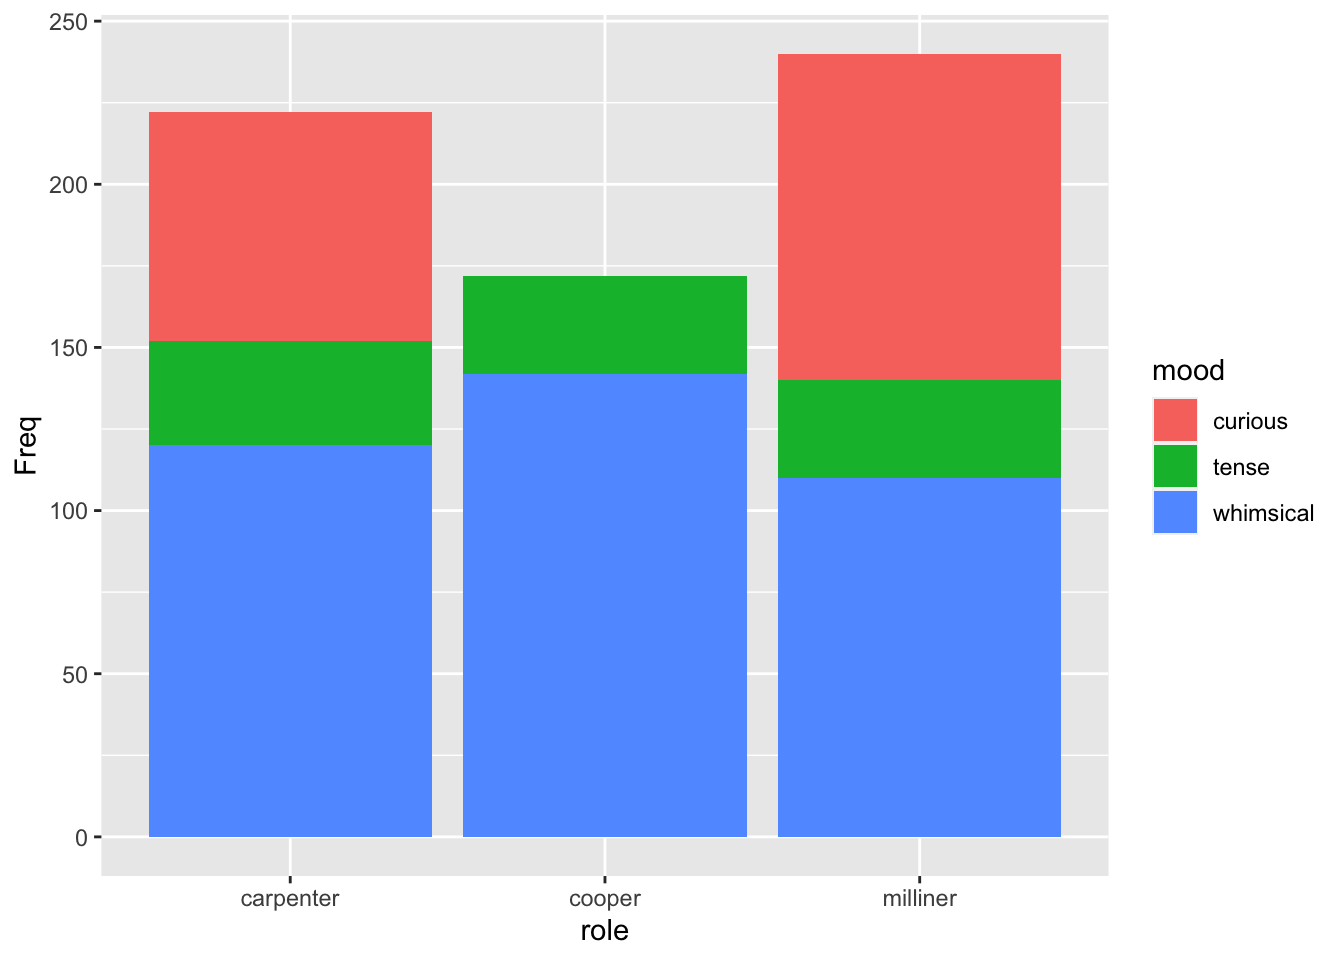
\includegraphics{intro_to_stats_files/figure-latex/unnamed-chunk-139-1.pdf}

This plot shows circles whose size is proportional to the count at each combination.

\hypertarget{heatmap}{%
\subsection{Heatmap}\label{heatmap}}

\begin{Shaded}
\begin{Highlighting}[]
\KeywordTok{ggplot}\NormalTok{(job_mood) }\OperatorTok{+}\StringTok{ }\KeywordTok{aes}\NormalTok{(mood, role) }\OperatorTok{+}\StringTok{ }\KeywordTok{geom_tile}\NormalTok{(}\KeywordTok{aes}\NormalTok{(}\DataTypeTok{fill=}\NormalTok{Freq))}
\end{Highlighting}
\end{Shaded}

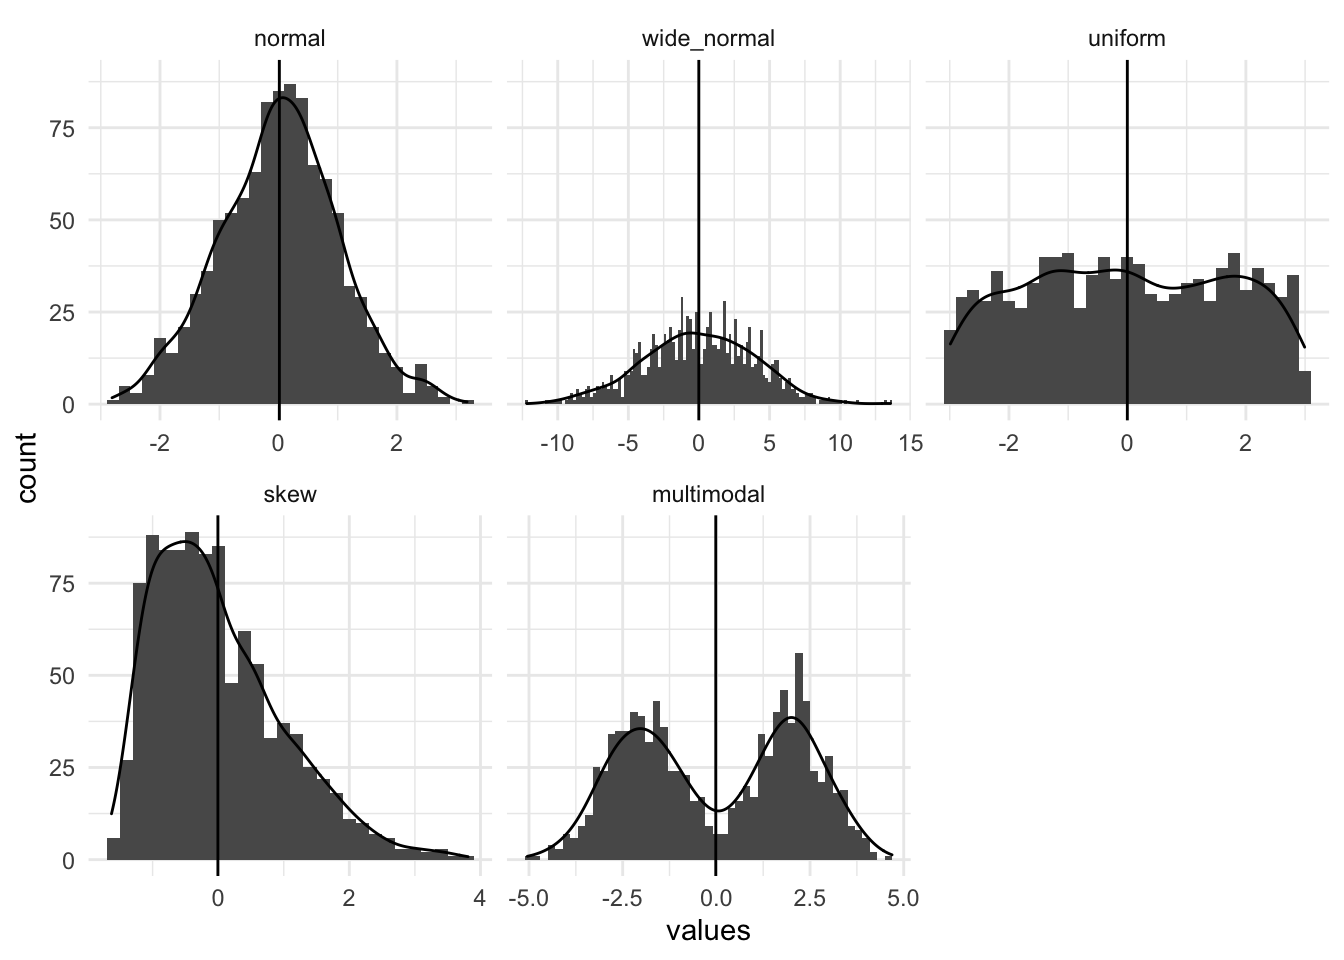
\includegraphics{intro_to_stats_files/figure-latex/unnamed-chunk-140-1.pdf}

This plot shows tiles whose filled colour represents the count at each combination

\hypertarget{stacked-bar}{%
\subsection{Stacked bar}\label{stacked-bar}}

\begin{Shaded}
\begin{Highlighting}[]
\KeywordTok{ggplot}\NormalTok{(job_mood) }\OperatorTok{+}\StringTok{ }\KeywordTok{aes}\NormalTok{(role, Freq) }\OperatorTok{+}\StringTok{ }\KeywordTok{geom_col}\NormalTok{(}\KeywordTok{aes}\NormalTok{(}\DataTypeTok{fill =}\NormalTok{ mood))}
\end{Highlighting}
\end{Shaded}

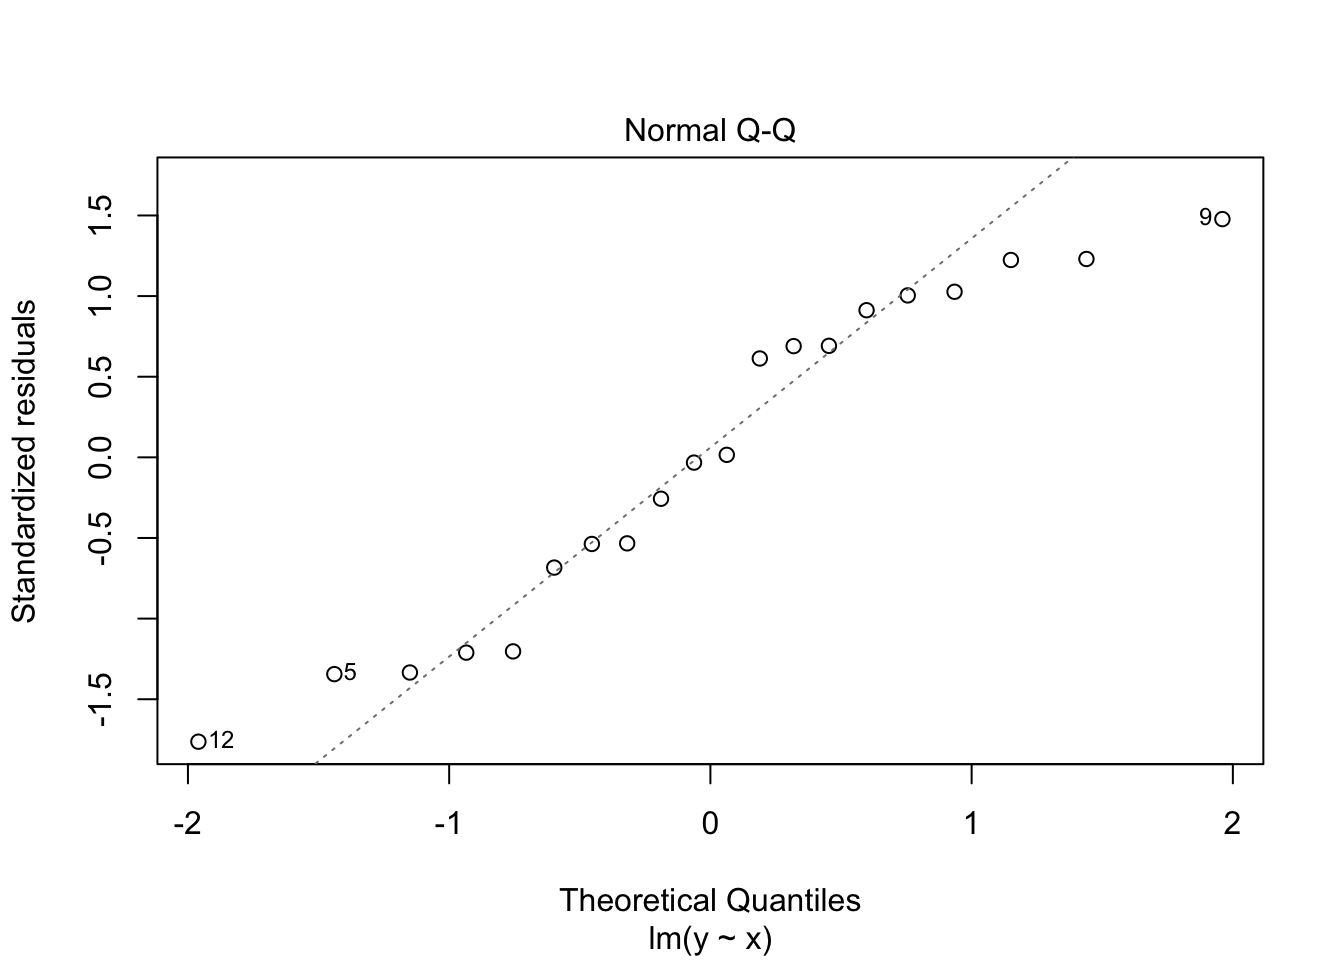
\includegraphics{intro_to_stats_files/figure-latex/unnamed-chunk-141-1.pdf}

\begin{roundup}
\begin{itemize}
\tightlist
\item
  Categoric explanatory (\(x\)) and response (\(y\)) variables are not amenable to use in linear models

  \begin{itemize}
  \tightlist
  \item
    In practice we are usually better off using the hypothesis tests
  \end{itemize}
\end{itemize}
\end{roundup}

\hypertarget{more-fun-with-linear-models}{%
\chapter{More fun with linear models}\label{more-fun-with-linear-models}}

\begin{enumerate}
\def\labelenumi{\arabic{enumi}.}
\tightlist
\item
  Questions
\end{enumerate}

\begin{itemize}
\tightlist
\item
  How do I know whether my model is any good?
\item
  How can I use the model to make predictions?
\item
  What can I use when linear models don't work well?
\end{itemize}

\begin{enumerate}
\def\labelenumi{\arabic{enumi}.}
\setcounter{enumi}{1}
\tightlist
\item
  Objectives
\end{enumerate}

\begin{itemize}
\tightlist
\item
  Learn how to tell whether the data you have are suitable for linear models
\item
  Learn how to make predictions from a model
\end{itemize}

\begin{enumerate}
\def\labelenumi{\arabic{enumi}.}
\setcounter{enumi}{2}
\tightlist
\item
  Keypoints
\end{enumerate}

\begin{itemize}
\tightlist
\item
  Data should be normally distributed, but linear models are quite robust to deviation from this
\item
  Models can be used to make new hypotheses
\item
  Linear models are one member of a larger family of models for many types of data
\end{itemize}

In this section we'll take a look at some extra features of linear models that it will be good to know about things that a linear model can do beyond looking for significant differences. We'll look at assessing whether a linear model is a good one, from a model fit point of view, we'll briefly discuss how to make predictions from linear models to guide hypothesis building and we'll briefly discuss the next level of linear model, the generalised linear model.

\hypertarget{assessing-a-linear-model}{%
\section{Assessing a linear model}\label{assessing-a-linear-model}}

A decent linear model fit to the data is essential for good statistical analysis with a linear model. The quality of fit to a linear model can be used to assess whether the data are appropriate for a particular test, even if we intend to just use the test. If we don't get a reliable fit we don't get a result we can be confident in from either the linear model and crucially, neither would we if we did the corresponding tests, like the \(t\)-test and ANOVA. Let's examine some model fits.

\hypertarget{the-terror-of-normality}{%
\subsection{The terror of normality}\label{the-terror-of-normality}}

Scientists that have done at least a little statistics often seem concerned that their data must be normally distributed for an analysis to be valid. This may stem from reviewers who will ask whether `the test is appropriate for the sort of data analysed' or related `whether the distribution of the data is normal'. These questions are sometimes legitimate, thankfully they are easy to answer and you should ask them of your data when you build your model because the answers will help you understand the goodness of your model. The good news is that you don't need to worry about your data being a super typical normal distribution, instead you can check whether the data are normal enough. All the tests and linear models will be very robust and even tend toward conservatism in their results if the data are all of the below:

\begin{enumerate}
\def\labelenumi{\arabic{enumi}.}
\tightlist
\item
  represented well by their mean
\item
  have a linear pattern in the residual
\item
  show a reasonable correlation in a qq-plot
\end{enumerate}

\hypertarget{checking-whether-the-mean-is-a-good-summary}{%
\subsection{Checking whether the mean is a good summary}\label{checking-whether-the-mean-is-a-good-summary}}

The first thing to check, whether you intend to do a simple \(t\)-test or a multi-way ANOVA is whether the mean is actually a good summary of the whole of the data. If you have multiple variables you'll need to check the means of each one. A mean is a good summary of a set of data if it sits nicely in the middle and there are no other peaks or skew in a histogram of that data. This is easier to think about if we draw some pictures. In this set of panels of histograms with density plots the mean (the vertical line) is an increasingly poor summary of the data as we go from left to right along the panels.

\begin{Shaded}
\begin{Highlighting}[]
\KeywordTok{library}\NormalTok{(itssl)}
\KeywordTok{its_is_the_mean_a_good_summary_time}\NormalTok{(}\DecValTok{1000}\NormalTok{, }\DataTypeTok{type =} \StringTok{"hist"}\NormalTok{)}
\end{Highlighting}
\end{Shaded}

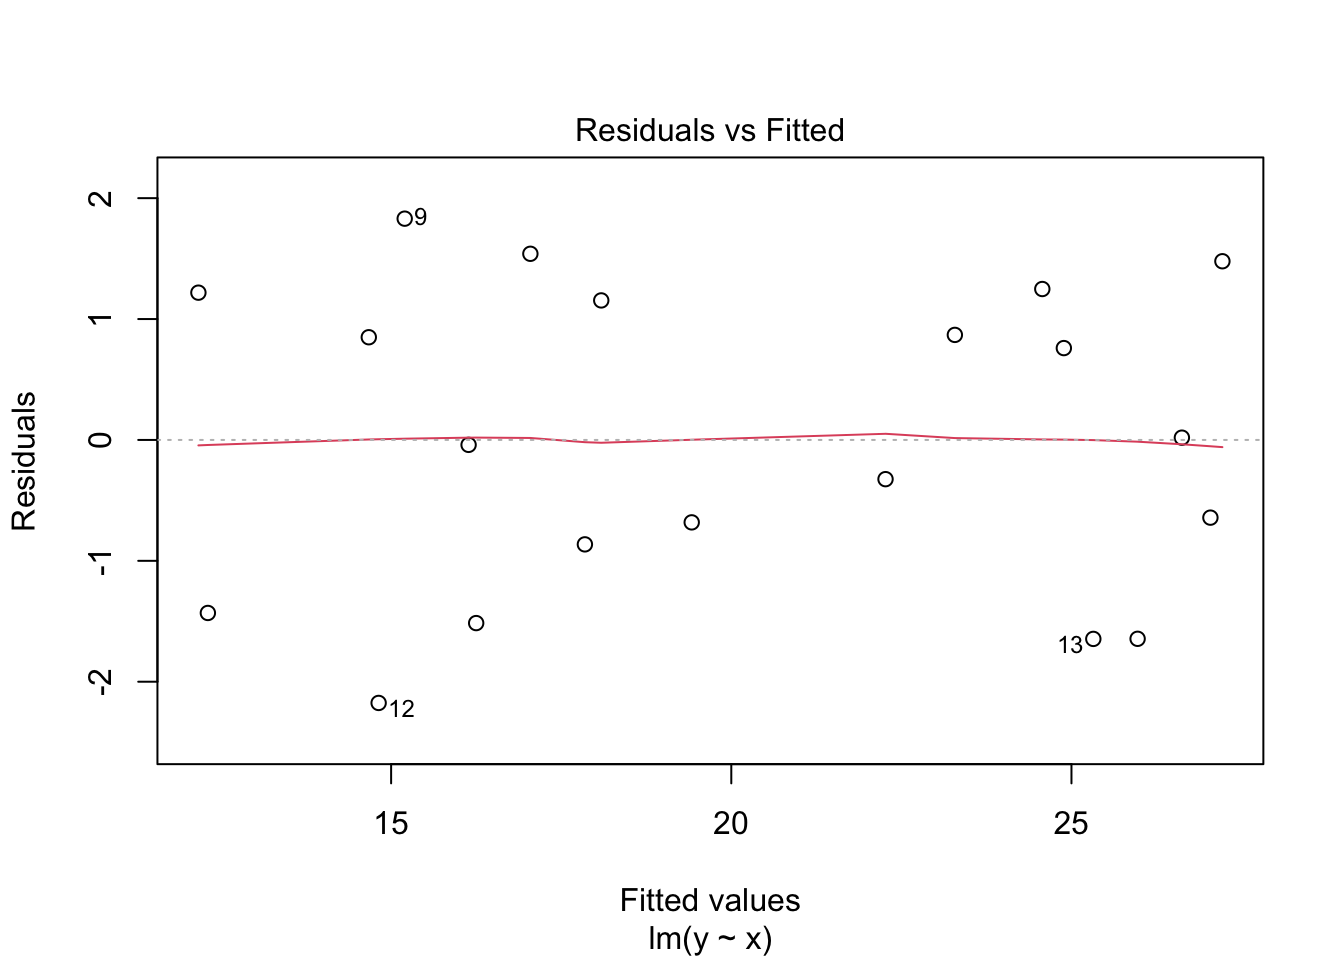
\includegraphics{intro_to_stats_files/figure-latex/unnamed-chunk-143-1.pdf}

The first two, a normal distribution and a normal distribution with a very wide standard deviation are summarised quite well by the mean. They have the mean at the peak, with the rest of the data falling evenly away. The third, the uniform distribution (in which all outcomes are equally likely) has no peak because the central outcome isn't more likely than the others so is less good, but still quite well summarised by the mean. The final two aren't nearly as well summarised well by the mean, the skew-normal distribution has the mean away from the peak because of the long tail and the multimodal has more than one peak. The take-home here is that the model fit and assumptions are increasingly poor as we move along, not that the tests and models become completely useless. In practice our conclusions must become more circumspect and a single test is less convincing.

\begin{task}
Use the tutorial to examine the effect of sample size on how these data look and view them in different plot type
\end{task}

\hypertarget{spotting-a-good-fit-to-the-data}{%
\subsection{Spotting a good fit to the data}\label{spotting-a-good-fit-to-the-data}}

Another thing you can do to assess your linear model is check out the residuals. Remember we described these as the distance between the actual data and the fitted line. The distribution of these tells us a lot. Let's think about these two data sets,

\begin{Shaded}
\begin{Highlighting}[]
\NormalTok{close_fit <-}\StringTok{ }\KeywordTok{its_random_xy_time}\NormalTok{(}\DecValTok{20}\NormalTok{)}
\NormalTok{far_fit <-}\StringTok{ }\KeywordTok{data.frame}\NormalTok{(}
\NormalTok{  x <-}\StringTok{ }\KeywordTok{runif}\NormalTok{(}\DecValTok{20}\NormalTok{, }\DecValTok{5}\NormalTok{, }\DecValTok{15}\NormalTok{),}
\NormalTok{  y <-}\StringTok{ }\KeywordTok{runif}\NormalTok{(}\DecValTok{20}\NormalTok{, }\DecValTok{5}\NormalTok{, }\DecValTok{15}\NormalTok{)}
\NormalTok{)}

\KeywordTok{its_plot_xy_time}\NormalTok{(close_fit, }\DataTypeTok{line =} \OtherTok{TRUE}\NormalTok{)}
\KeywordTok{its_plot_xy_time}\NormalTok{(far_fit, }\DataTypeTok{line =} \OtherTok{TRUE}\NormalTok{)}
\end{Highlighting}
\end{Shaded}

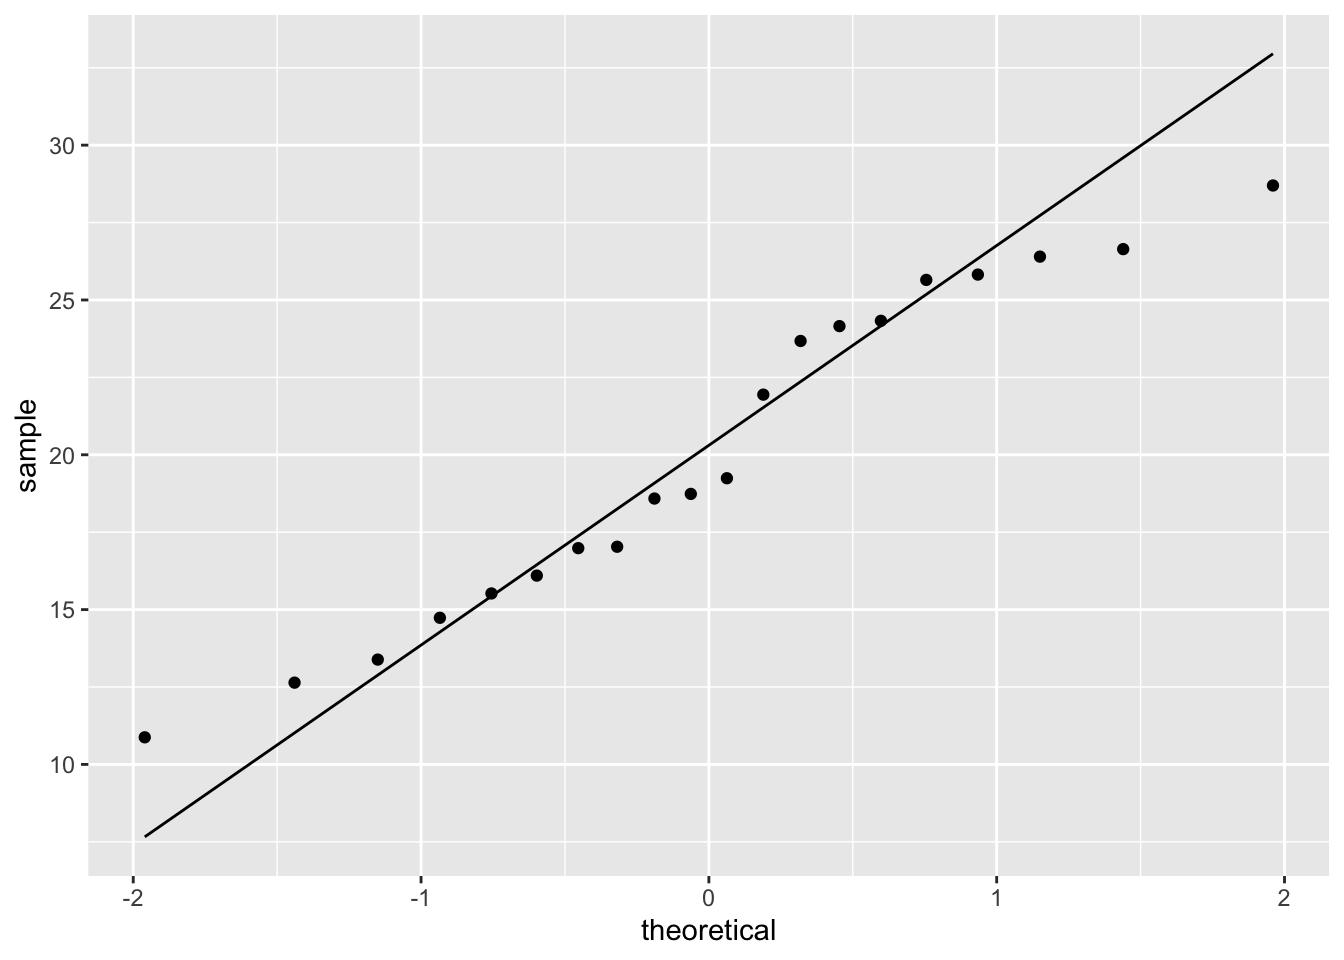
\includegraphics[width=0.5\linewidth]{intro_to_stats_files/figure-latex/unnamed-chunk-145-1} 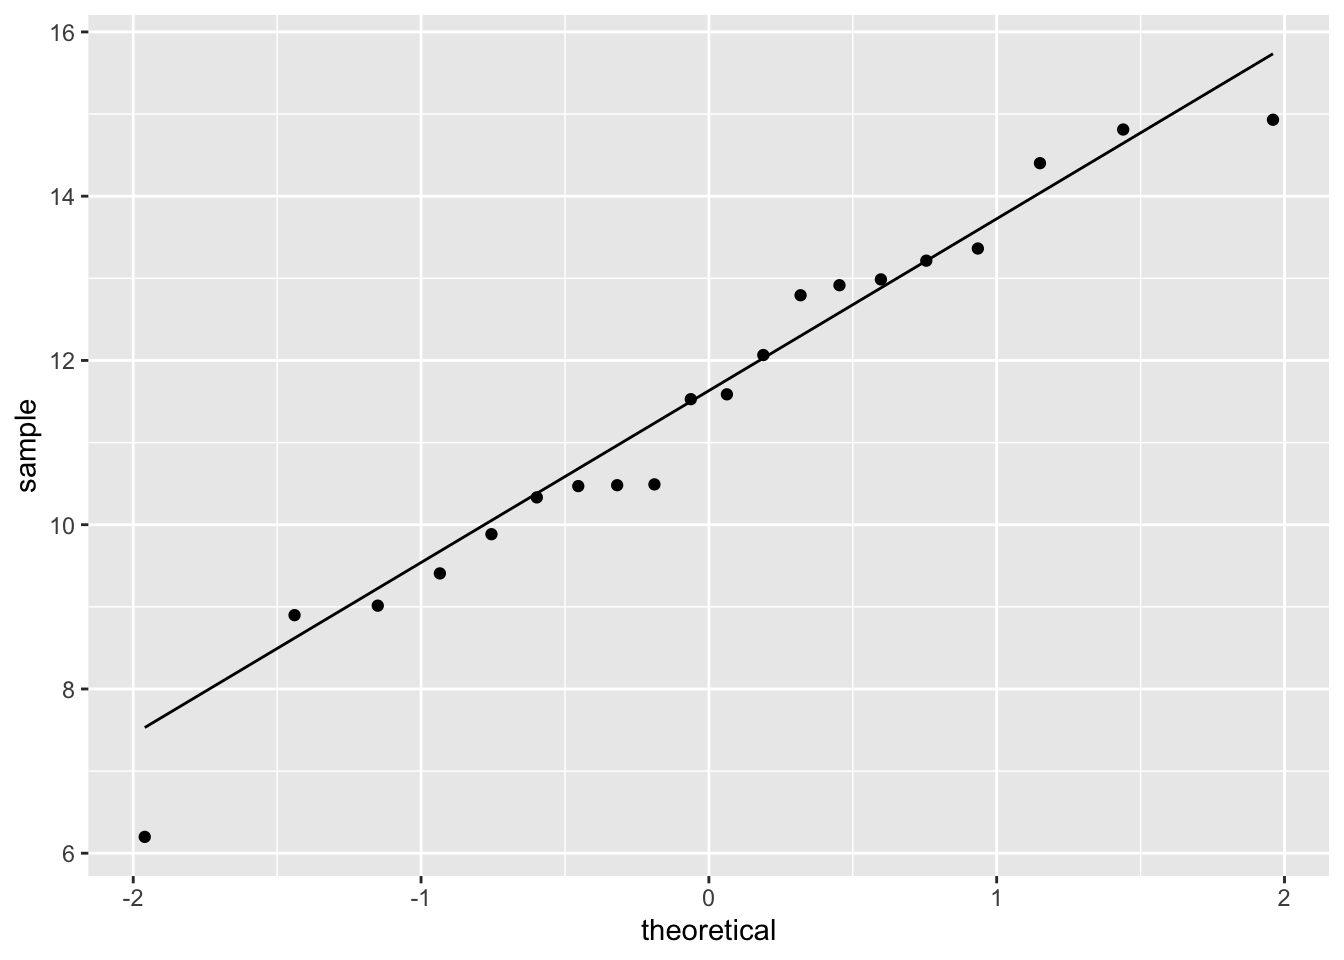
\includegraphics[width=0.5\linewidth]{intro_to_stats_files/figure-latex/unnamed-chunk-145-2}

We can see the first has a fairly good slope and the points are all relatively close to the line, while in the second the slope is weak because the points are further away. The \texttt{lm()} function calculates the residuals and we can plot them.

\begin{Shaded}
\begin{Highlighting}[]
\NormalTok{close_fit_model <-}\StringTok{ }\KeywordTok{lm}\NormalTok{(y }\OperatorTok{~}\StringTok{ }\NormalTok{x, }\DataTypeTok{data =}\NormalTok{ close_fit)}
\NormalTok{far_fit_model <-}\StringTok{ }\KeywordTok{lm}\NormalTok{(y }\OperatorTok{~}\StringTok{ }\NormalTok{x, }\DataTypeTok{data =}\NormalTok{ far_fit)}

\KeywordTok{plot}\NormalTok{(close_fit_model, }\DataTypeTok{which =} \DecValTok{1}\NormalTok{)}
\KeywordTok{plot}\NormalTok{(far_fit_model, }\DataTypeTok{which =} \DecValTok{1}\NormalTok{)}
\end{Highlighting}
\end{Shaded}

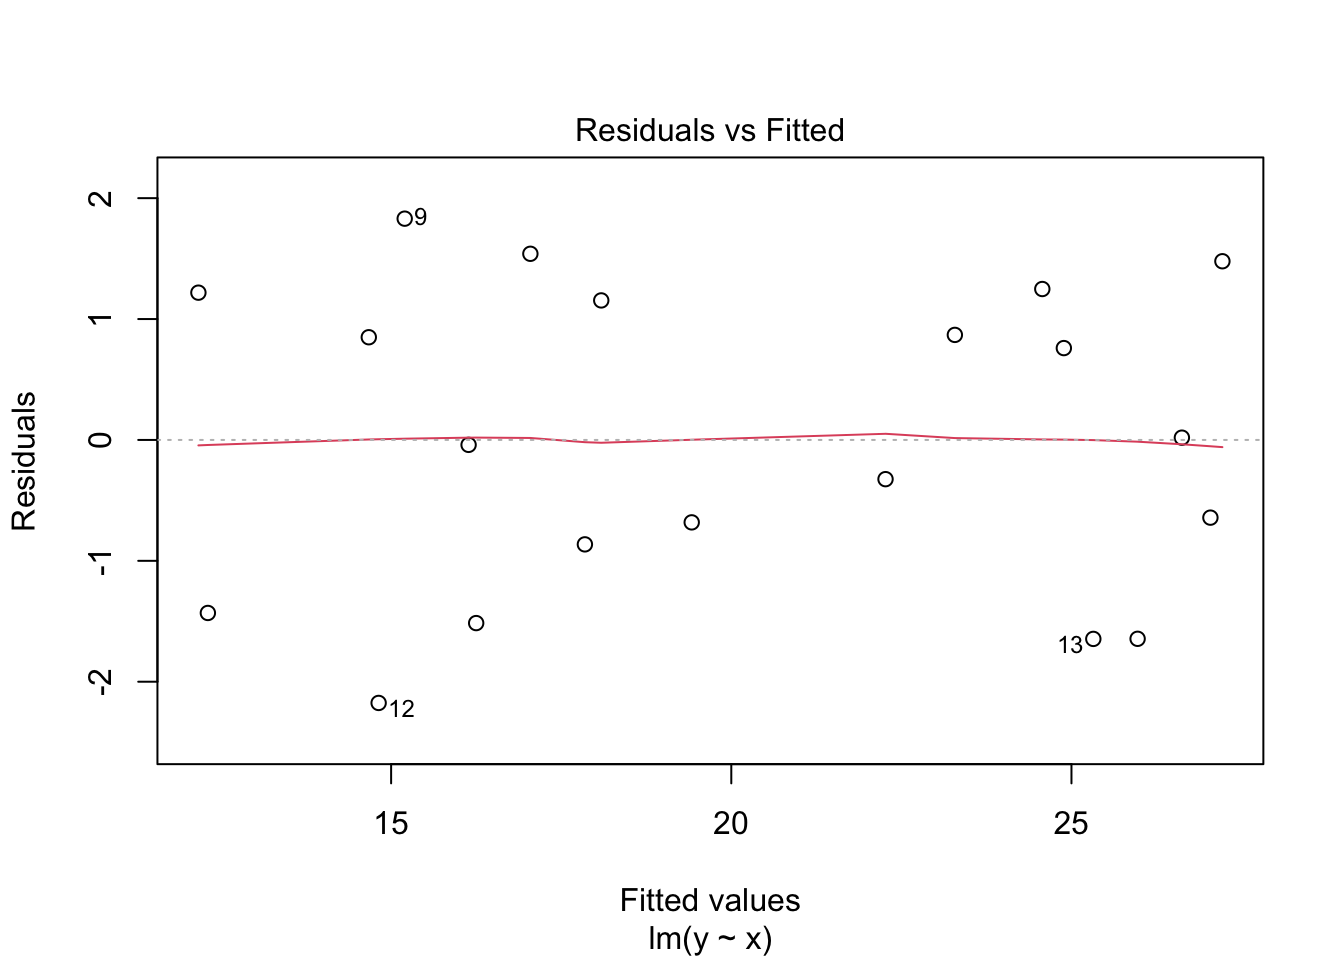
\includegraphics[width=0.5\linewidth]{intro_to_stats_files/figure-latex/unnamed-chunk-146-1} 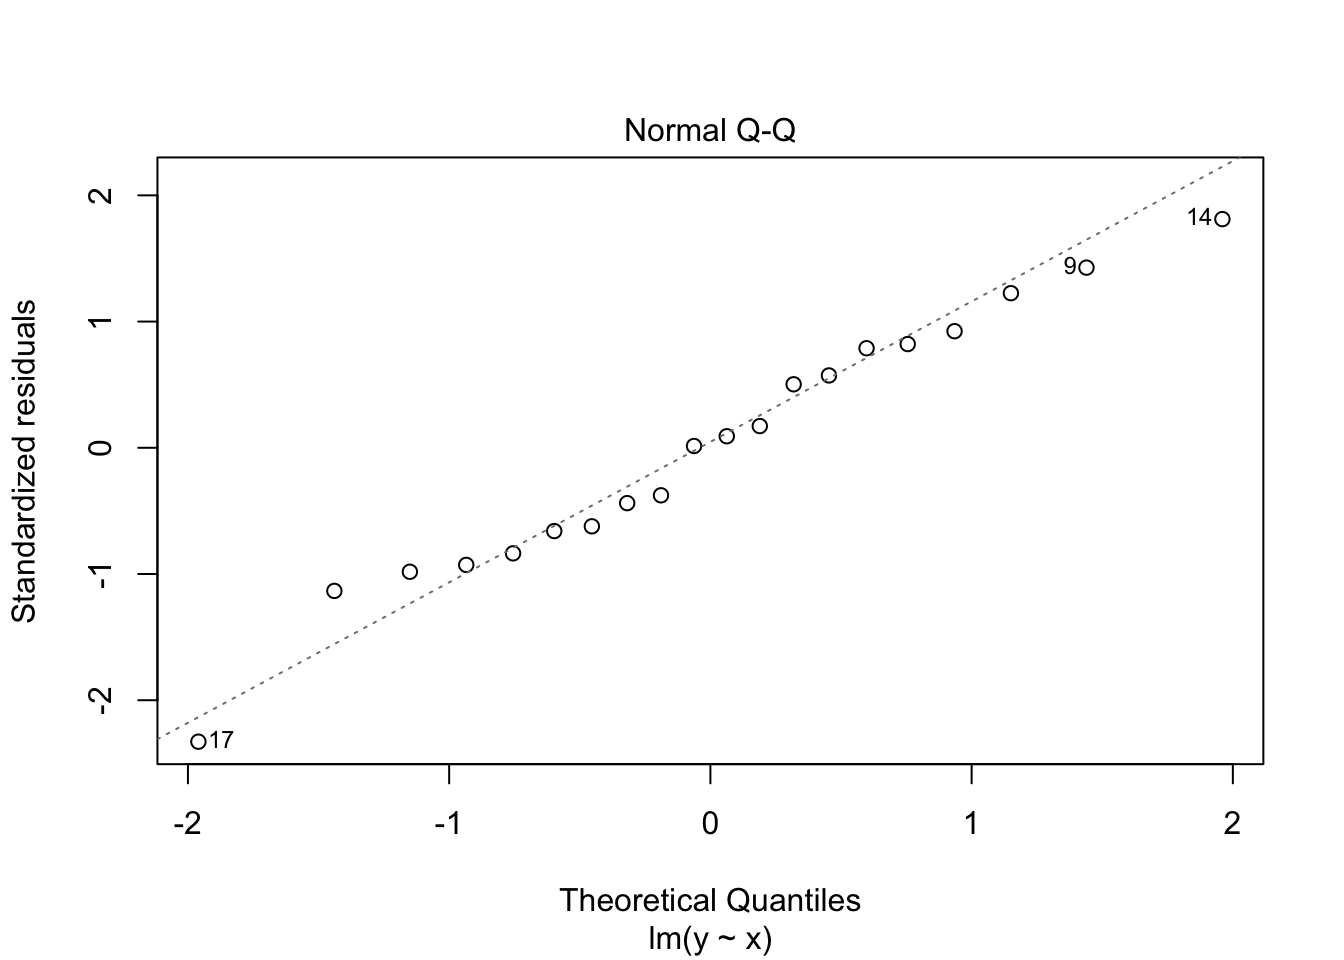
\includegraphics[width=0.5\linewidth]{intro_to_stats_files/figure-latex/unnamed-chunk-146-2}

Here we see the \(x\)-axis value is the value from the model, so the \(x\)-axis value of a data point, the \(y\)-axis value is the residual itself the distance between the line \(y\) value and the observed \(y\) value. The first plot shows a nice even scatter and flat line and a range of -2 to 2. The second shows a more erratic scatter with the red line having a little wobble and a much higher range, from - 6 to 4.

Together they show us that the second model doesn't fit as the data as closely as the first, the increased residual size and the more wobbly line mean it isn't as good. Its still not useless though, a wobbly line is still sometimes useable, we would be more worried if we had these data, which have some hidden structure in. Here's a non-linear data set and its residual plot

\begin{Shaded}
\begin{Highlighting}[]
\NormalTok{non_linear_data <-}\StringTok{ }\NormalTok{tibble}\OperatorTok{::}\KeywordTok{tibble}\NormalTok{(}
  \DataTypeTok{x =} \DecValTok{1}\OperatorTok{:}\DecValTok{20}\NormalTok{,}
  \DataTypeTok{y =}\NormalTok{ (x }\OperatorTok{^}\StringTok{ }\DecValTok{2}\NormalTok{ ) }\OperatorTok{+}\StringTok{ }\KeywordTok{runif}\NormalTok{(}\DecValTok{20}\NormalTok{, }\DecValTok{3}\NormalTok{, }\DecValTok{60}\NormalTok{)}
\NormalTok{)}

\KeywordTok{its_plot_xy_time}\NormalTok{(non_linear_data, }\DataTypeTok{line =} \OtherTok{TRUE}\NormalTok{)}

\NormalTok{non_linear_model <-}\StringTok{ }\KeywordTok{lm}\NormalTok{(y }\OperatorTok{~}\StringTok{ }\NormalTok{x, }\DataTypeTok{data =}\NormalTok{ non_linear_data)}
\KeywordTok{plot}\NormalTok{(non_linear_model, }\DataTypeTok{which =} \DecValTok{1}\NormalTok{)}
\end{Highlighting}
\end{Shaded}

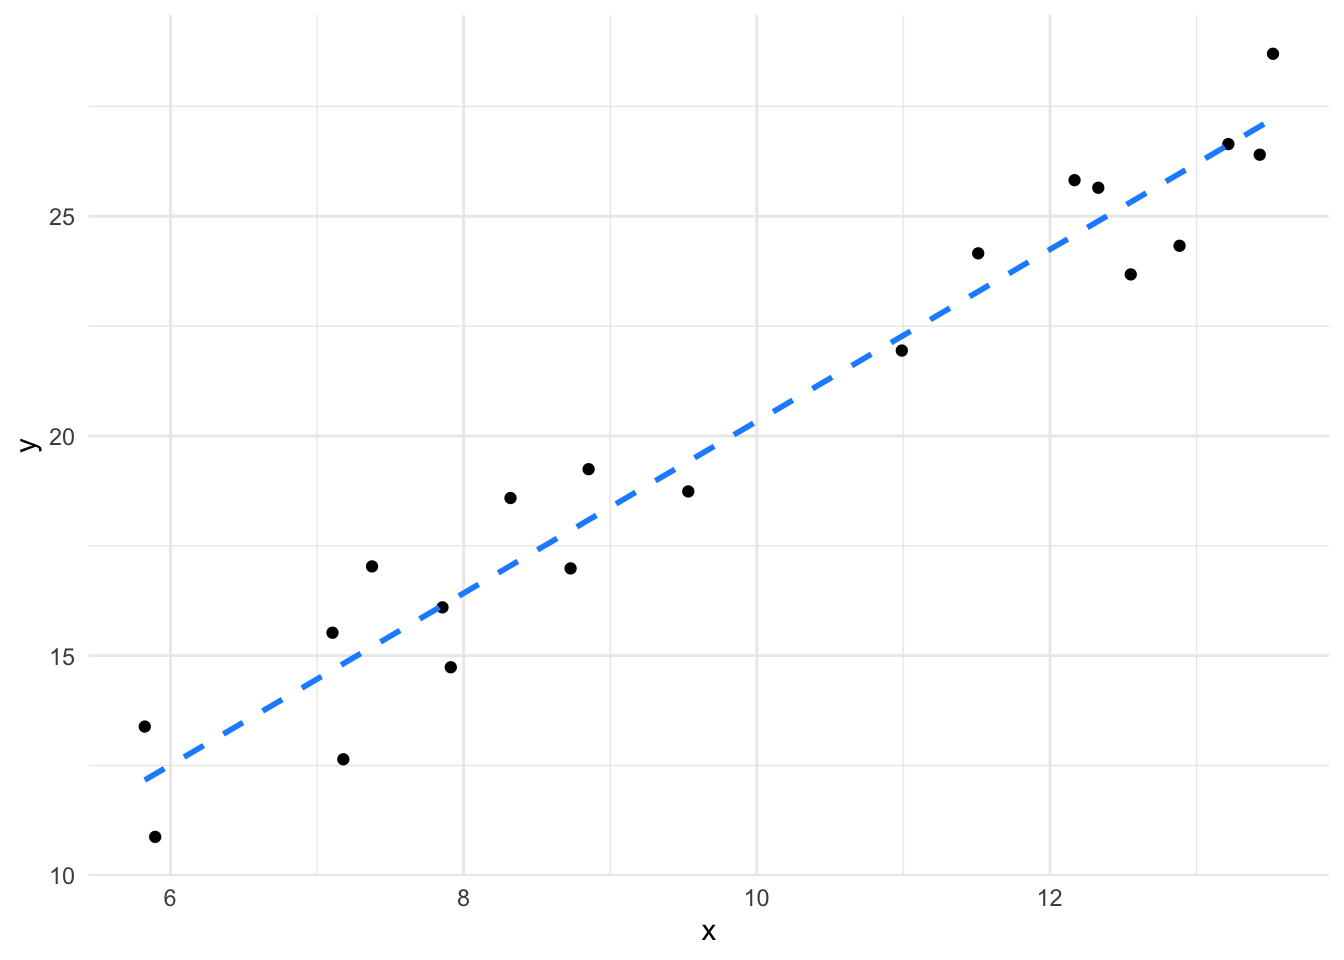
\includegraphics[width=0.5\linewidth]{intro_to_stats_files/figure-latex/unnamed-chunk-147-1} \includegraphics[width=0.5\linewidth]{intro_to_stats_files/figure-latex/unnamed-chunk-147-2}

Initially, the line seems to fit the data quite well, but the giveaway is in the residual plot, which has quite the pattern!! The data are actually a \(y = x^2\) relationship with some noise added. By viewing the \(x\) vs \(y\) plot we don't easily see that relationship, but the residuals very definitely show that the linear model doesn't fit the data well, the structure in the residual plot indicates that the model is failing to capture some part of our data. As you might imagine, linear models (and related tests) performed with non-linear data will not give good results.

\hypertarget{checking-qq-plots-for-a-normal-distribution}{%
\subsection{Checking qq-plots for a normal distribution}\label{checking-qq-plots-for-a-normal-distribution}}

The qq-plot tests the question of whether data are normally distributed directly. Here the \(x\) values are basically random numbers drawn from a normal distribution with mean and standard deviation the same as the model data and the \(y\) values are the real data. This is easy to do with \texttt{ggplot()}

\begin{Shaded}
\begin{Highlighting}[]
\KeywordTok{library}\NormalTok{(ggplot2)}
\KeywordTok{ggplot}\NormalTok{(close_fit) }\OperatorTok{+}\StringTok{ }\KeywordTok{aes}\NormalTok{(}\DataTypeTok{sample =}\NormalTok{ y) }\OperatorTok{+}\StringTok{ }\KeywordTok{stat_qq}\NormalTok{() }\OperatorTok{+}\StringTok{ }\KeywordTok{stat_qq_line}\NormalTok{()}
\KeywordTok{ggplot}\NormalTok{(far_fit) }\OperatorTok{+}\StringTok{ }\KeywordTok{aes}\NormalTok{(}\DataTypeTok{sample =}\NormalTok{ y) }\OperatorTok{+}\StringTok{ }\KeywordTok{stat_qq}\NormalTok{() }\OperatorTok{+}\StringTok{ }\KeywordTok{stat_qq_line}\NormalTok{()}
\KeywordTok{ggplot}\NormalTok{(non_linear_data) }\OperatorTok{+}\StringTok{ }\KeywordTok{aes}\NormalTok{(}\DataTypeTok{sample =}\NormalTok{ y) }\OperatorTok{+}\StringTok{ }\KeywordTok{stat_qq}\NormalTok{() }\OperatorTok{+}\StringTok{ }\KeywordTok{stat_qq_line}\NormalTok{()}
\end{Highlighting}
\end{Shaded}

\includegraphics[width=0.33\linewidth]{intro_to_stats_files/figure-latex/unnamed-chunk-148-1} \includegraphics[width=0.33\linewidth]{intro_to_stats_files/figure-latex/unnamed-chunk-148-2} \includegraphics[width=0.33\linewidth]{intro_to_stats_files/figure-latex/unnamed-chunk-148-3}

These often deviate at the ends of the scatter plot, but the centre parts should fall along the line with random deviation. Here, with these particular data sets, the \texttt{close\_fit} and \texttt{far\_fit} appear to be matching marginally better overall than the \texttt{non\_linear} which is veering around the line quite a lot.

and again, we can also do this with the residual data which should also be normally distributed, here the \texttt{lm()} function does a lot of the work for us.

\begin{Shaded}
\begin{Highlighting}[]
\KeywordTok{plot}\NormalTok{(close_fit_model, }\DataTypeTok{which =} \DecValTok{2}\NormalTok{)}
\KeywordTok{plot}\NormalTok{(far_fit_model, }\DataTypeTok{which =} \DecValTok{2}\NormalTok{)}
\KeywordTok{plot}\NormalTok{(non_linear_model, }\DataTypeTok{which =} \DecValTok{2}\NormalTok{)}
\end{Highlighting}
\end{Shaded}

\includegraphics[width=0.33\linewidth]{intro_to_stats_files/figure-latex/unnamed-chunk-149-1} \includegraphics[width=0.33\linewidth]{intro_to_stats_files/figure-latex/unnamed-chunk-149-2} \includegraphics[width=0.33\linewidth]{intro_to_stats_files/figure-latex/unnamed-chunk-149-3}

\hypertarget{predictions}{%
\section{Predictions}\label{predictions}}

Sometimes we will want to use our existing data to build hypotheses for testing with new experiments. The linear model can be used to aid this by using it as a tool to predict what the model outputs would be given a particular set of inputs across the variables that we used to build our model. In this section we'll take a look at doing things like predicting new data on our response (\(y\)-axis) given some \(x\) values.

\hypertarget{intuition-on-prediction-from-continuous-variables}{%
\subsection{Intuition on prediction from continuous variables}\label{intuition-on-prediction-from-continuous-variables}}

The intuition behind this is more straightforward than you might initially think, consider the straight lines from our first section. We had a continuous \(x\) and \(y\) axis

\begin{Shaded}
\begin{Highlighting}[]
\NormalTok{df <-}\StringTok{ }\KeywordTok{its_random_xy_time}\NormalTok{(}\DecValTok{20}\NormalTok{)}
\KeywordTok{its_plot_xy_time}\NormalTok{(df, }\DataTypeTok{line =} \OtherTok{TRUE}\NormalTok{)}
\end{Highlighting}
\end{Shaded}

\includegraphics{intro_to_stats_files/figure-latex/unnamed-chunk-150-1.pdf}

We can peek into \(x\) to see what values we \emph{actually} used

\begin{Shaded}
\begin{Highlighting}[]
\KeywordTok{sort}\NormalTok{(df}\OperatorTok{$}\NormalTok{x)}
\end{Highlighting}
\end{Shaded}

\begin{verbatim}
##  [1]  5.824327  5.895516  7.105123  7.179086  7.375033  7.855269  7.912222
##  [8]  8.319600  8.729459  8.852362  9.532381 10.989182 11.510336 12.167571
## [15] 12.329553 12.551050 12.883979 13.216811 13.431172 13.521335
\end{verbatim}

Although we don't have a real \(x = 10\) in our data, imagine asking the question ``what \(y\) would we get for \(x = 10\)?''. We can intuitively tell what the \(y\)-value would be simply by reading off the line at \(x = 10\), which is about 20 or from the formula, \(y = (1.9555 * 10) + 0.7780 = 20.33\). This is the intuition behind how a linear model prediction works with continuous \(x\) and \(y\) - we're just reading off the line.

If we build the model, we can ask it to work this out for us directly using the \texttt{predict()} function. \texttt{predict()} takes the model and the new values to be predicted in a \texttt{data.frame}.

\begin{Shaded}
\begin{Highlighting}[]
\NormalTok{model <-}\StringTok{ }\KeywordTok{lm}\NormalTok{(y }\OperatorTok{~}\StringTok{ }\NormalTok{x, }\DataTypeTok{data =}\NormalTok{ df)}
\KeywordTok{predict}\NormalTok{(model, }\DataTypeTok{newdata =} \KeywordTok{data.frame}\NormalTok{(}\DataTypeTok{x =} \KeywordTok{c}\NormalTok{(}\DecValTok{10}\NormalTok{)))}
\end{Highlighting}
\end{Shaded}

\begin{verbatim}
##        1 
## 20.33266
\end{verbatim}

We see that we get the same value (given a little rounding error).

What happens when we give the \texttt{predict()} function a value we did have data for? Let's pull out whatever the fifth value of our data was and look at that

\begin{Shaded}
\begin{Highlighting}[]
\NormalTok{df}\OperatorTok{$}\NormalTok{x[}\DecValTok{5}\NormalTok{]}
\end{Highlighting}
\end{Shaded}

\begin{verbatim}
## [1] 12.88398
\end{verbatim}

\begin{Shaded}
\begin{Highlighting}[]
\NormalTok{df}\OperatorTok{$}\NormalTok{y[}\DecValTok{5}\NormalTok{]}
\end{Highlighting}
\end{Shaded}

\begin{verbatim}
## [1] 24.32715
\end{verbatim}

This shows us that the \(x\) axis value of 12.88 had the corresponding \(y\) value of 24.33. Now let's use the model to predict the \(y\) from the \(x\)

\begin{Shaded}
\begin{Highlighting}[]
\NormalTok{vals_to_predict <-}\StringTok{ }\KeywordTok{data.frame}\NormalTok{(}\DataTypeTok{x =} \KeywordTok{c}\NormalTok{(df}\OperatorTok{$}\NormalTok{x[}\DecValTok{5}\NormalTok{]))}
\KeywordTok{predict}\NormalTok{(model, }\DataTypeTok{newdata =}\NormalTok{ vals_to_predict)}
\end{Highlighting}
\end{Shaded}

\begin{verbatim}
##        1 
## 25.97217
\end{verbatim}

The result from the model is quite different from the actual observed data value! This isn't an error. Its because we're asking the model to predict using the `line' it came up with. Note that this is because the prediction comes from the model which takes into account the whole data. This is the process of `best fitting' which ensures the `line' matches all the points as well as possible, but doesn't guarantee matching any particular point well.

\begin{sidenote}
It is possible to over-complicate models to make them fit all the points by allowing them to take extra parameters and become curves. Adding complexity in this way usually leads to bad models that only fit one particular data set well and is called `overfitting'.
\end{sidenote}

\hypertarget{prediction-intervals}{%
\subsubsection{Prediction intervals}\label{prediction-intervals}}

If you are going to predict a value, you might want instead an interval in which that prediction might lie with certain amount of certainty. Like a confidence interval for the position of the mean in a sample, a prediction interval is a range that we are most certain a prediction will land in. This interval takes in the range of spread in the data we build the linear model with and turns it into something useless. Once the model is built, it's easy to use the \texttt{predict()} function to get the prediction interval

\begin{Shaded}
\begin{Highlighting}[]
\NormalTok{vals_to_predict <-}\StringTok{ }\KeywordTok{data.frame}\NormalTok{( }\DataTypeTok{x =} \KeywordTok{c}\NormalTok{(}\DecValTok{10}\NormalTok{) )}
\KeywordTok{predict}\NormalTok{(model, }\DataTypeTok{newdata =}\NormalTok{ vals_to_predict, }\DataTypeTok{interval =} \StringTok{"predict"}\NormalTok{)}
\end{Highlighting}
\end{Shaded}

\begin{verbatim}
##        fit      lwr      upr
## 1 20.33266 17.52743 23.13788
\end{verbatim}

we can see the predicted value and the lower and upper bounds of the prediction interval.

\hypertarget{intuition-on-prediction-with-categoric-variables}{%
\subsection{Intuition on prediction with categoric variables}\label{intuition-on-prediction-with-categoric-variables}}

In the same way we looked at the line to get an intuitive understanding of how the linear model makes predictions, we can look at the groups in a categorical variable to see how \(y\) values are predicted from factors.

Consider the \texttt{chickwts} data.

\begin{Shaded}
\begin{Highlighting}[]
\KeywordTok{its_plot_chickwts_time}\NormalTok{()}
\end{Highlighting}
\end{Shaded}

\includegraphics{intro_to_stats_files/figure-latex/unnamed-chunk-158-1.pdf}

We can see that in this data set there is a single categorical variable called \texttt{feed} which is the type of food the chick was raised on, and the resulting continuous output variable of \texttt{weight}. If we model that and do a prediction we can get an intuition on what the \texttt{prediction()} means for each category.

\begin{Shaded}
\begin{Highlighting}[]
\NormalTok{model <-}\StringTok{ }\KeywordTok{lm}\NormalTok{(weight }\OperatorTok{~}\StringTok{ }\NormalTok{feed, }\DataTypeTok{data =}\NormalTok{ chickwts)}
\KeywordTok{predict}\NormalTok{(model,}\DataTypeTok{newdata =} \KeywordTok{data.frame}\NormalTok{(}\DataTypeTok{feed =} \KeywordTok{c}\NormalTok{(}\StringTok{"casein"}\NormalTok{)))}
\end{Highlighting}
\end{Shaded}

\begin{verbatim}
##        1 
## 323.5833
\end{verbatim}

\begin{Shaded}
\begin{Highlighting}[]
\KeywordTok{predict}\NormalTok{(model,}\DataTypeTok{newdata =} \KeywordTok{data.frame}\NormalTok{(}\DataTypeTok{feed =} \KeywordTok{c}\NormalTok{(}\StringTok{"sunflower"}\NormalTok{)))}
\end{Highlighting}
\end{Shaded}

\begin{verbatim}
##        1 
## 328.9167
\end{verbatim}

Note that this time we have to use the a level of a factor, because that was the only term in this model. It doesn't make sense to give it a number. The model returns the fitted value of \texttt{weight} for the level of the factor.

Do the numbers returned remind you of anything? Aren't they awfully close to where we expect the mean of each group to be. Let's check that out by doing a prediction for each feed and comparing with the group mean.

\begin{Shaded}
\begin{Highlighting}[]
\CommentTok{#first get a vector of the chickwts feed names}
\NormalTok{feeds <-}\StringTok{ }\KeywordTok{sort}\NormalTok{(}\KeywordTok{unique}\NormalTok{(chickwts}\OperatorTok{$}\NormalTok{feed))}
\CommentTok{#do the prediction}
\NormalTok{preds <-}\StringTok{ }\KeywordTok{predict}\NormalTok{(model,}\DataTypeTok{newdata =} \KeywordTok{data.frame}\NormalTok{(}\DataTypeTok{feed =}\NormalTok{ feeds) )}
\CommentTok{#add the names for clarity}
\KeywordTok{names}\NormalTok{(preds) <-}\StringTok{  }\NormalTok{feeds}

\NormalTok{preds}
\end{Highlighting}
\end{Shaded}

\begin{verbatim}
##    casein horsebean   linseed  meatmeal   soybean sunflower 
##  323.5833  160.2000  218.7500  276.9091  246.4286  328.9167
\end{verbatim}

Now calculating the mean from the data.

\begin{Shaded}
\begin{Highlighting}[]
\KeywordTok{library}\NormalTok{(dplyr)}
\KeywordTok{group_by}\NormalTok{(chickwts, feed) }\OperatorTok\StringTok{ }
\StringTok{  }\KeywordTok{summarize}\NormalTok{(}\DataTypeTok{mean =} \KeywordTok{mean}\NormalTok{(weight)) }
\end{Highlighting}
\end{Shaded}

\begin{verbatim}
## # A tibble: 6 x 2
##   feed       mean
##   <fct>     <dbl>
## 1 casein     324.
## 2 horsebean  160.
## 3 linseed    219.
## 4 meatmeal   277.
## 5 soybean    246.
## 6 sunflower  329.
\end{verbatim}

Yep, they're the same. This gives us the intuition that for the model of categoric data the prediction for each group in the category is the centre of it. It may not always be the exact mean, but it's a useful way of thinking about it.

\hypertarget{using-predictions-in-more-complicated-models}{%
\subsection{Using predictions in more complicated models}\label{using-predictions-in-more-complicated-models}}

A significant use of predictions is when we have a mixture of variables that we can't easily just see the mean for and want to know what the model thinks of those. This is especially useful for hypothesis generation or finding out possible parameter ranges for new experiments. As the last thing we'll do with predictions we'll look at the \texttt{txhousing} data, a data set about housing in Texas. This data has a mixture of continuous and categoric variables. We'll see that this it isn't more complicated than prediction for a single variable but does give us a much more convenient and powerful way to predict an outcome from provided values.

First a quick look at \texttt{txhousing}

\begin{Shaded}
\begin{Highlighting}[]
\KeywordTok{str}\NormalTok{(txhousing)}
\end{Highlighting}
\end{Shaded}

\begin{verbatim}
## tibble [8,602 x 9] (S3: tbl_df/tbl/data.frame)
##  $ city     : chr [1:8602] "Abilene" "Abilene" "Abilene" "Abilene" ...
##  $ year     : int [1:8602] 2000 2000 2000 2000 2000 2000 2000 2000 2000 2000 ...
##  $ month    : int [1:8602] 1 2 3 4 5 6 7 8 9 10 ...
##  $ sales    : num [1:8602] 72 98 130 98 141 156 152 131 104 101 ...
##  $ volume   : num [1:8602] 5380000 6505000 9285000 9730000 10590000 ...
##  $ median   : num [1:8602] 71400 58700 58100 68600 67300 66900 73500 75000 64500 59300 ...
##  $ listings : num [1:8602] 701 746 784 785 794 780 742 765 771 764 ...
##  $ inventory: num [1:8602] 6.3 6.6 6.8 6.9 6.8 6.6 6.2 6.4 6.5 6.6 ...
##  $ date     : num [1:8602] 2000 2000 2000 2000 2000 ...
\end{verbatim}

Now let's build a linear model of property sale price predicted by the city it is in and the year and month of sale.

\begin{Shaded}
\begin{Highlighting}[]
\NormalTok{model <-}\StringTok{ }\KeywordTok{lm}\NormalTok{(median }\OperatorTok{~}\StringTok{ }\NormalTok{city }\OperatorTok{+}\StringTok{ }\NormalTok{year }\OperatorTok{+}\StringTok{ }\NormalTok{month, }\DataTypeTok{data =}\NormalTok{ txhousing)}
\end{Highlighting}
\end{Shaded}

And finally get a prediction for a particular case.

\begin{Shaded}
\begin{Highlighting}[]
\KeywordTok{predict}\NormalTok{(model, }\DataTypeTok{newdata =} \KeywordTok{data.frame}\NormalTok{(}\DataTypeTok{city =} \KeywordTok{c}\NormalTok{(}\StringTok{"Abilene"}\NormalTok{), }\DataTypeTok{year =} \KeywordTok{c}\NormalTok{(}\DecValTok{2000}\NormalTok{), }\DataTypeTok{month =} \KeywordTok{c}\NormalTok{(}\DecValTok{2}\NormalTok{)))}
\end{Highlighting}
\end{Shaded}

\begin{verbatim}
##       1 
## 65392.3
\end{verbatim}

This shows how the linear model can be used to make predictions and hypothesis for further work.

\hypertarget{generalized-linear-models}{%
\section{Generalized Linear Models}\label{generalized-linear-models}}

Generalized Linear Models (GLMs) are, as the name might suggest, a generalization of the linear model that can be used when the residuals are not normally distributed. We went to quite a lot of trouble in this chapter to learn how to identify normally distributed residuals and input data and to press home the idea that if we do have data that look mostly normal then the linear model is still a useful tool. However, there are many situations where your data isn't going to be anything like normal and that's where a GLM is helpful. GLMs are particularly useful instance in non-linear situations like exponentially changing data or count data, indeed in earlier chapters we did see some data that definitely didn't fit a normal (though we didn't point it out explicitly at the time) the frequency data in the \(\chi^2\) test section wasn't usable in a linear model without a great deal of fiddling.

\begin{sidenote}
Actually, with a lot of non-normal data, e.g exponential data, we can `hack' our data to be more normal by applying a transformation such as taking logs, and then proceed as before. Often we can't or shouldn't and that's where Generalized Linear Models come in.
\end{sidenote}

GLMs can be thought of as clever linear models that you can specify the type of distribution the residual has, this means the mathematics is a lot more complicated, but in practice it's just another function in R - \texttt{glm()} which is related to \texttt{lm()} and works much like it with some extra options to set.

GLMs are a powerful thing and great to know about, and once you've got the hang of linear models not terribly hard to use, keep them in mind as you work through your analyses and if you come across a data set that doesn't seem to fit well with linear models, maybe you need to move over to a GLM.

\begin{roundup}
\begin{itemize}
\tightlist
\item
  Linear models work best when the residuals are normally distributed, but linear models are somewhat robust to deviation from this

  \begin{itemize}
  \tightlist
  \item
    Models can be used to make new hypotheses
  \item
    Linear models are one member of a larger family of models for many types of data, Generalized Linear models are the general class of tool.
  \end{itemize}
\end{itemize}
\end{roundup}

  \bibliography{book.bib,packages.bib,citations.bib}

\end{document}
